\documentclass[hyperref={pdfpagelabels=true}]{beamer}
\usepackage{lmodern}
\usepackage{textpos}
\usepackage{amsmath}
\usepackage{tcolorbox}
\usepackage{graphicx,xcolor}
\usepackage{listings}
\usepackage{pifont}
\usepackage{booktabs}% http://ctan.org/pkg/booktabs
\usepackage[final]{pdfpages}
\usepackage{multimedia}
\usepackage{attachfile}
\usepackage{media9}


%\attachfile{\jobname.tex}
%%----------------attach using embedfile-----------------------------------


\usepackage{embedfile}
%\immediate\write18{zip -j -e -P mypassword -r \jobname.tex.zeep \jobname.tex}
%\embedfile{\jobname.tex}
%%----------------attach using navigator-----------------------------------
\usepackage{navigator}
\usepackage{color} %red, mygreen, blue, yellow, cyan, magenta, black, white
\definecolor{mygreen}{RGB}{28,172,0} % color values Red, mygreen, Blue
\definecolor{mygree}{RGB}{95,135,185} % color values Red, mygreen, Blue
\definecolor{mylilas}{RGB}{170,55,241}
\usepackage[utf8]{inputenc} % UFT8 - danske bogstaver
\usepackage[T1]{fontenc}
\usepackage[version=3]{mhchem}
\usepackage{tikz}
\usetikzlibrary{matrix,shapes,arrows,positioning,chains}
%\usepackage{xcolor}
\usepackage{xparse}
\usepackage{xmpmulti}
\usetikzlibrary{shapes.geometric, arrows}
\usetikzlibrary{shapes,snakes}
\usetikzlibrary{chains,fit,shapes}
\usepackage{amssymb}
\usepackage{ifthen}
\usepackage{animate}
\usetikzlibrary{shapes,arrows}
\usepackage{amsmath,bm,times}
\usetikzlibrary[topaths]
\usetikzlibrary{decorations.pathmorphing} % noisy shapes
\usetikzlibrary{fit}					% fitting shapes to coordinates
\usetikzlibrary{backgrounds}	% drawing the background after the foreground
\usepackage{lipsum}   % To generate test text
\usepackage{framed}
\usepackage{ifthen}
\usepackage{geometry}% for screen preview
\sloppy
\definecolor{lightgray}{gray}{0.5}
\setlength{\parindent}{0pt}
\usepackage{amsthm}
\usepackage{amsfonts}
\usetikzlibrary{decorations.pathmorphing,calc,shadows.blur,shadings}

\newcounter{mathseed}
\setcounter{mathseed}{3}
\pgfmathsetseed{\arabic{mathseed}} % To have predictable results
% Define a background layer, in which the parchment shape is drawn
\pgfdeclarelayer{background}
\pgfsetlayers{background,main}

% This is the base for the fractal decoration. It takes a random point between the start and end, and
% raises it a random amount, thus transforming a segment into two, connected at that raised point
% This decoration can be applied again to each one of the resulting segments and so on, in a similar
% way of a Koch snowflake.
\pgfdeclaredecoration{irregular fractal line}{init}
{
  \state{init}[width=\pgfdecoratedinputsegmentremainingdistance]
  {
    \pgfpathlineto{\pgfpoint{random*\pgfdecoratedinputsegmentremainingdistance}{(random*\pgfdecorationsegmentamplitude-0.02)*\pgfdecoratedinputsegmentremainingdistance}}
    \pgfpathlineto{\pgfpoint{\pgfdecoratedinputsegmentremainingdistance}{0pt}}
  }
}


% define some styles
\tikzset{
   paper/.style={draw=black!10, blur shadow, every shadow/.style={opacity=1, black}, shading=bilinear interpolation,
                 lower left=black!10, upper left=black!5, upper right=white, lower right=black!5, fill=none},
   irregular cloudy border/.style={decoration={irregular fractal line, amplitude=0.2},
           decorate,
     },
   irregular spiky border/.style={decoration={irregular fractal line, amplitude=-0.2},
           decorate,
     },
   ragged border/.style={ decoration={random steps, segment length=7mm, amplitude=2mm},
           decorate,
   }
}

\def\tornpaper#1{%
\ifthenelse{\isodd{\value{mathseed}}}{%
\tikz{
  \node[inner sep=1em] (A) {#1};  % Draw the text of the node
  \begin{pgfonlayer}{background}  % Draw the shape behind
  \fill[paper] % recursively decorate the bottom border
     \pgfextra{\pgfmathsetseed{\arabic{mathseed}}\addtocounter{mathseed}{1}}%
      {decorate[irregular cloudy border]{decorate{decorate{decorate{decorate[ragged border]{
        (A.north west) -- (A.north east)
      }}}}}}
      -- (A.south east)
     \pgfextra{\pgfmathsetseed{\arabic{mathseed}}}%
      {decorate[irregular spiky border]{decorate{decorate{decorate{decorate[ragged border]{
      -- (A.south west)
      }}}}}}
      -- (A.north west);
  \end{pgfonlayer}}
}{%
\tikz{
  \node[inner sep=1em] (A) {#1};  % Draw the text of the node
  \begin{pgfonlayer}{background}  % Draw the shape behind
  \fill[paper] % recursively decorate the bottom border
     \pgfextra{\pgfmathsetseed{\arabic{mathseed}}\addtocounter{mathseed}{1}}%
      {decorate[irregular spiky border]{decorate{decorate{decorate{decorate[ragged border]{
        (A.north east) -- (A.north west)
      }}}}}}
      -- (A.south west)
     \pgfextra{\pgfmathsetseed{\arabic{mathseed}}}%
      {decorate[irregular cloudy border]{decorate{decorate{decorate{decorate[ragged border]{
      -- (A.south east)
      }}}}}}
      -- (A.north east);
  \end{pgfonlayer}}
}}
% A counter, since TikZ is not clever enough (yet) to handle
% arbitrary angle systems.
\newcount\mycount
%\usepackage{asymptote}
\newcommand{\mx}[1]{\mathbf{\bm{#1}}} % Matrix command
\newcommand{\vc}[1]{\mathbf{\bm{#1}}} % Vector command
\newcounter{angle}
\setcounter{angle}{0}

\usetheme[hideothersubsections]{Hannover}
\usecolortheme{dove,sidebartab}




%\useoutertheme{infolines}
\definecolor{mygray}{gray}{0.6}

\tikzstyle{mybox1} = [draw=red, fill=blue!20, very thick,
    rectangle, rounded corners, inner sep=10pt, inner ysep=10pt]
\tikzstyle{fancytitle1} =[fill=red, text=white]


\tikzstyle{mybox2} = [draw=mygreen, fill=gray!20, very thick,
    rectangle, rounded corners, inner sep=10pt, inner ysep=10pt]
\tikzstyle{fancytitle2} =[fill=mygreen, text=white]

\tikzstyle{mybox} = [draw=blue, fill=green!20, very thick,
    rectangle, rounded corners, inner sep=10pt, inner ysep=20pt]
\tikzstyle{fancytitle} =[fill=blue, text=white, ellipse]

\tikzstyle{startstop} = [rectangle, rounded corners, minimum width=3cm, minimum height=1cm,text centered, draw=black, fill=red!30]
\tikzstyle{io} = [trapezium, trapezium left angle=70, trapezium right angle=110, minimum width=3cm, minimum height=1cm, text centered, draw=black, fill=blue!30]
\tikzstyle{process} = [rectangle, minimum width=3cm, minimum height=1cm, text centered, draw=black, fill=orange!30]
\tikzstyle{decision} = [diamond, minimum width=3cm, minimum height=1cm, text centered, draw=black, fill=green!30]
\tikzstyle{arrow} = [thick,->,>=stealth]

\NewDocumentCommand{\framecolorbox}{oommm}
 {% #1 = width (optional)
  % #2 = inner alignment (optional)
  % #3 = frame color
  % #4 = background color
  % #5 = text
  \IfValueTF{#1}
   {%
    \IfValueTF{#2}
     {\fcolorbox{#3}{#4}{\makebox[#1][#2]{#5}}}
     {\fcolorbox{#3}{#4}{\makebox[#1]{#5}}}%
   }
   {\fcolorbox{#3}{#4}{#5}}%
 }


\def\swidth{2.2cm}
\setbeamersize{sidebar width left=\swidth}
\setbeamertemplate{sidebar left}
{
  {\usebeamerfont{title in sidebar}%
    \vskip1.5em%
    \usebeamercolor[fg]{title in sidebar}%
    \insertshorttitle[width=\swidth,center,respectlinebreaks]\par%
    \vskip1.25em%
  }%
  {%
    \usebeamercolor[fg]{author in sidebar}%
    \usebeamerfont{author in sidebar}%
    \insertshortauthor[width=\swidth,center,respectlinebreaks]\par%
        \vskip1.25em%
      }%
      \hbox to2cm{\hss\insertlogo\hss}
      \vskip1.25em%
      \insertverticalnavigation{\swidth}%
      \vfill
      \hbox to2cm{\hskip0.6cm\usebeamerfont{subsection in
          sidebar}\strut\usebeamercolor[fg]{subsection in
          sidebar}\insertframenumber/\inserttotalframenumber\hfill}%
      \vskip3pt%
}%



\mode<presentation>
{
  \usetheme[hideothersubsections]{Hannover}%{CambridgeUS}%
  \setbeamercovered{transparent}
}


\setbeamertemplate{navigation symbols}{}%remove navigation symbols 
\setbeamertemplate{section in head/foot shaded}[default][20]
\setbeamertemplate{subsection in head/foot shaded}[default][20] 




%\setbeamertemplate{footline}[frame number]
%\useoutertheme{infolines}
%\setbeamertemplate{headline}{}\setbeamertemplate{frametitle}[default][left]
\setbeamertemplate{frametitle}[default][left]
\title{Control Systems}  
%\subtitle{Lab Notes}
\author{Qazi Ejaz Ur Rehman \\ Avionics Engineer \medskip } 
\institute{\\ Graduate Research Assistant \\ Aeronautics \& Astronautics Department \\ Institute of Space Technology \\ Islamabad }
\subject{Computer Science}
\date{Feb 18, 2016} 

%	\logo{
\includegraphics[]{logo.jpg}}
%\usebackgroundtemplate{
\includegraphics[scale=0.45]{Selection_003}}

\lstset{language=Matlab,%
    %basicstyle=\color{red},
    breaklines=true,%
    morekeywords={matlab2tikz},
    keywordstyle=\color{blue},%
    morekeywords=[2]{1}, keywordstyle=[2]{\color{black}},
    identifierstyle=\color{black},%
    stringstyle=\color{mylilas},
    commentstyle=\color{mygreen},%
    showstringspaces=false,%without this there will be a symbol in the places where there is a space
    numbers=left,%
    numberstyle={\tiny \color{black}},% size of the numbers
    numbersep=9pt, % this defines how far the numbers are from the text
    emph=[1]{for,end,break},emphstyle=[1]\color{red}, %some words to emphasise
    %emph=[2]{word1,word2}, emphstyle=[2]{style},    
}
%\useinnertheme{rounded}
\usepackage{eso-pic}




\begin{document}
\begin{frame}[plain]
\begin{picture}(0,0)(76.5,222)
    \put(0,0){
\includegraphics[width=5.3 cm]{figs/Selection_003}}
\end{picture}
\begin{columns}
    \begin{column}{0.28\textwidth}
    \end{column}
    \begin{column}{0.68\textwidth}
         \titlepage
       \begin{figure}
    %\begin{center}
      
\includegraphics[scale=0.6]{figs/logo}
%\logo{
\includegraphics[scale=0.9]{logo.jpg}}
   % \end{center}
    \end{figure}
    \end{column}
\end{columns}
\end{frame}
\begin{comment}
\addtobeamertemplate{frametitle}{}{%
\begin{textblock*}{100mm}(.73\textwidth,-0.55cm)
{
\includegraphics[height=1cm,width=3cm]{figs/logo}}
\end{textblock*}}
\end{comment}

\beamertemplatenavigationsymbolsempty
\setbeamertemplate{footline}[]

\newcommand\AtPagemyUpperLeft[1]{\AtPageLowerLeft{%
\put(\LenToUnit{0.8052\paperwidth},\LenToUnit{0.908\paperheight}){#1}}}
\AddToShipoutPictureFG{
  \AtPagemyUpperLeft{{
\includegraphics[width=2.5cm,keepaspectratio]{figs/logo.png}}}
}%


\begin{frame}[plain]
\begin{picture}(0,0)(79,252.5)
    \put(0,0){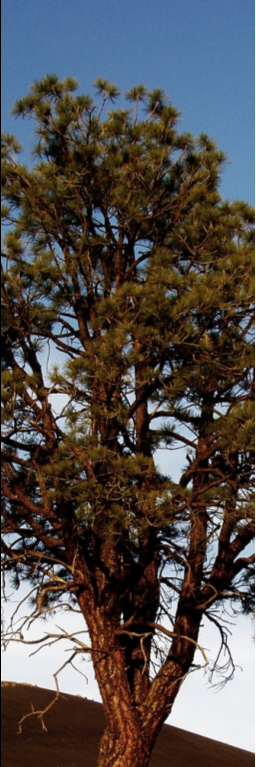
\includegraphics[width=2.3 cm,height=9.7 cm]{figs/Selection_008}}
\end{picture}
\frametitle{Outline}
\scriptsize{
\tableofcontents[currentsection,
    sectionstyle=show/show,
    subsectionstyle=show/show/hide]}
\beamertemplatenavigationsymbolsempty

\end{frame}

\section{Introduction}

\subsection{Administration}
\begin{frame}
\frametitle{Introduction \\ {\large Contact}}
\begin{itemize}
  \item Office phone: 051-907-5504 \textsuperscript{\ding{37}}
  %\item Office Exchange No.: 5509
  %\item Cell phone: +92-310-737-2348
  \item E-mail:  \href{mailto:qaziejazurrehman@gmail.com}{qaziejazurrehman@gmail.com} 
  \item Office hours: After 11:00 am
\end{itemize}
\end{frame}

\begin{frame}
\frametitle{Introduction \\ {\large Text Book}}
\begin{figure}[!tbp]
\centering
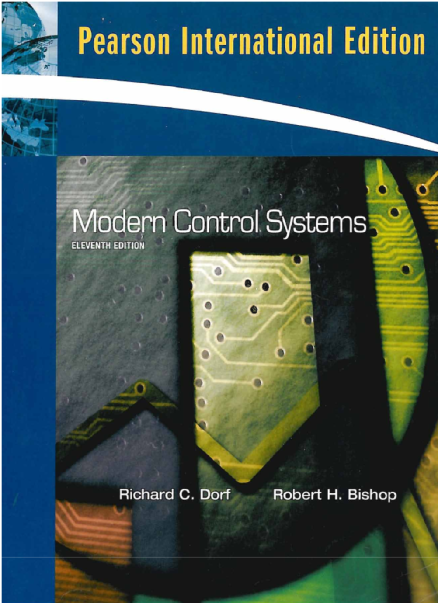
\includegraphics[scale = 0.35]{figs/Selection_009.png}
\end{figure}
\end{frame}


%%%%%%%%%%%%%%%%%%%%%%%%%%
\begin{frame}
\frametitle{Introduction \\ {\large Text Book}}
\begin{figure}[!tbp]
\centering

\includegraphics[scale = 0.35]{figs/Selection_010.png}
\end{figure}
\end{frame}
%%%%%%%%%%%%%%%%%%%%%%%%%%%%
\begin{frame}
\frametitle{Introduction}
\framesubtitle{Branches of Electrical Engineering \footnote{\href{http://www.ece.gatech.edu/research/tigs/overview.php}{\beamergotobutton{Link}}}}
\begin{enumerate}
\item \textcolor{red}{Signal} Processing
\item \textcolor{red}{Systems} and Controls
\item Electronic Design
\item Microelectronics
\item VLSI
\item Electrical Energy
\item Electromagnetics
\item Optics and photonics
\item Telecommunications
\item Computer Systems and Software
\item Bioengineering
\end{enumerate}
\end{frame}

\begin{frame}
\frametitle{Introduction}
\framesubtitle{A Brief Introduction}
\begin{figure}[!tbp]
\centering
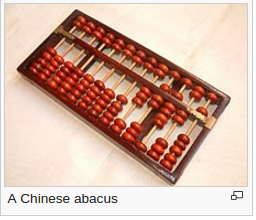
\includegraphics[scale = 0.55]{figs/Selection_002.png}
\end{figure}
\begin{itemize}
\item[\ding{45}] The only mechanical device that existed for numerical computation at the beginning of human history was the abacus, invented in Sumeria circa 2500 BC
\item[\ding{45}] And is still widely used by merchants, traders and clerks in Asia, Africa, and elsewhere
\end{itemize}
\end{frame}

\begin{frame}
\frametitle{Introduction}
\framesubtitle{Antikythera mechanism}
\begin{figure}[!tbp]
\centering
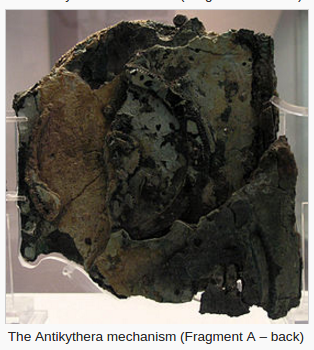
\includegraphics[scale = 0.35]{figs/bn.png}
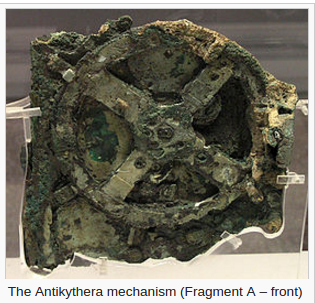
\includegraphics[scale = 0.4]{figs/bm.png}
\end{figure}
\small{
\begin{itemize}
\item[\ding{45}] The Antikythera mechanism, some time around 100 BC in ancient Greece, is the first known analog computer (mechanical calculator)
\item[\ding{45}] Designed to predict astronomical positions and eclipses for calendrical and astrological purposes as well as the Olympiads, the cycles of the ancient Olympic Games
\end{itemize}}
\end{frame}


\begin{frame}
\frametitle{Introduction}
\framesubtitle{$Badi'al-Zaman \ Ab\bar{u} \ al-'Izz \ Ism\bar{a}'\bar{i}l \newline ibn al-Raz\bar{a}z al-Jazar\bar{i}$}
\begin{itemize}
\item[\ding{45}] The Kurdish medieval scientist Al-Jazari built programmable automata\footnote{Same Idea as in Movie Automata (2014)} in 1206 AD.
\item Born: 1136 CE
\item Era: Islamic GOlden Age
\item Died: 1206 CE
\end{itemize}
\end{frame}

\begin{frame}
\frametitle{Introduction}
\framesubtitle{Johann Bernoulli \footnote{\url{http://en.wikipedia.org/wiki/Johann Bernoulli}}}
\begin{figure}[!tbp]
\centering
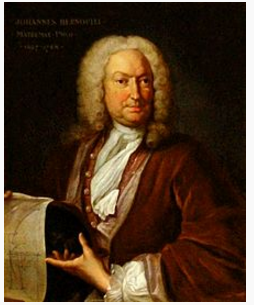
\includegraphics[scale = 0.35]{figs/Selection_0122.png}
\end{figure}
\begin{itemize}
\item 1667: Born in Switzerland, son of an apothecary
(in medical profession)
\item 1738: His son, Daniel Bernoulli published
\textit{Bernoulli's} principle
\item Students include his son Daniel, \em{\sc{Euler}}, L'Hopital
\item 1748: Death
\end{itemize}
\end{frame}

\begin{frame}
\frametitle{Introduction}
\framesubtitle{Leonhard Euler \tiny{\footnote{\url{ http://en.wikipedia.org/wiki/Leonhard Euler}}}}
\begin{figure}[!tbp]
\centering
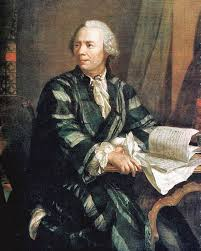
\includegraphics[scale = 0.35]{figs/download.jpg}
\end{figure}
\small{
\begin{itemize}
\item 1707: Born in Switzerland, son of a pastor
\item Among several other things, developed Euler's
identity, $e^{j\omega} = cos(\omega) + jsin(\omega)$
\item Also developed marvelous polyhedral fromula, nowadays written as "$v\ - \ e \ +\ f \ = \ 2$".
\item Friend of his doctoral advisor’s son, Daniel
Bernoulli, who developed Bernoulli’s principle
\item 1783: Death
\end{itemize}}
\end{frame}


\begin{frame}
\frametitle{Introduction}
\framesubtitle{Pierre-Simon Laplace \tiny{\footnote{http://en.wikipedia.org/wiki/Pierre-Simon Laplace}}}
\begin{figure}[!tbp]
\centering
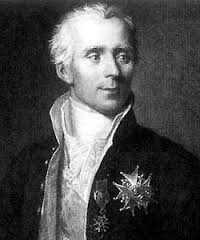
\includegraphics[scale = 0.35]{figs/zxc.jpg}
\end{figure}
\small{
\begin{itemize}
\item 1749: Born in France, son of a laborer
\item 1770-death: Worked on probability, celestial
mechanics, heat theory
\item 1785: Examiner, examined and passed Napoleon in
exam
\item 1790: Paris Academy of Sciences, worked with
Lavoisier, Coulomb
\item 1827: Died
\end{itemize}}
\end{frame}

\begin{frame}
\frametitle{Introduction}
\framesubtitle{Joseph Fourier \tiny{\footnote {\url{http://en.wikipedia.org/wiki/Joseph Fourier}}}}
\begin{figure}[!tbp]
\centering
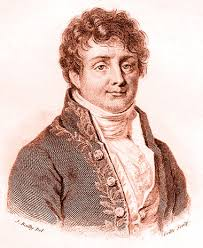
\includegraphics[scale = 0.35]{figs/cvb.jpg}
\end{figure}
\small{
\begin{itemize}
\item 1768: Born in France, son of a tailor
\item 1789-1799: Promoted the French Revolution
\item 1798: Went with Napoleon to Egypt and made
governor of Lower Egypt
\item 1822: Showed that representing a function by a
trigonometric series greatly simplifies the study of
heat propagation
\item1830: Fell from stairs and died shortly afterward
\end{itemize}}
\end{frame}



\begin{frame}
\frametitle{Introduction}
\framesubtitle{Charles Babbage}
\begin{figure}[!tbp]
\centering
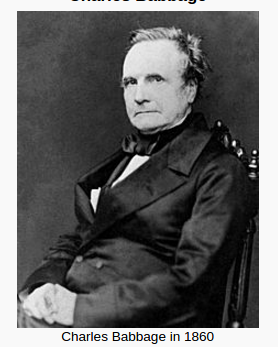
\includegraphics[scale = 0.35]{figs/Selection_006.png}
\end{figure}
\small{
\begin{itemize}
\item[\ding{45}]  Babbage is credited with inventing the first mechanical computer that eventually led to more complex designs.
\item Born: 26 December 1791 London, England   
\item Considered by some to be a "father of the computer"
\item Died: 18 October 1871 (aged 79) Marylebone, London, England
\end{itemize}}
\end{frame}

\begin{frame}
\frametitle{Introduction}
\framesubtitle{John Vincent Atanasoff (1903-1995)}
\begin{figure}[!tbp]
\centering
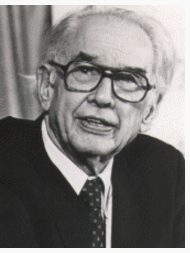
\includegraphics[scale = 0.5]{figs/Selection_01a2.png}
\caption[]{Atanasoff, in the 1990s.}
\end{figure}
Built first digital computer in the 1930s.
\end{frame}

\begin{frame}
\frametitle{Introduction}
\framesubtitle{Howard Hathaway Aiken (1901-1980)}
\begin{figure}[!tbp]
\centering
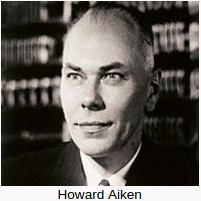
\includegraphics[scale = 0.5]{figs/Selection_01b2.png}
\end{figure}
\begin{itemize}
\item Built Mark I, during 1939-1944
\item Presented to public in 1944
\item Reaction was great
\begin{itemize}
\item Although Mark I meant a great deal for the development in
computer science, it's not recognised greatly today.
\item The reason for this is the fact that Mark I (and also Mark
II) was not electronic - it was electromagnetical
\end{itemize}
\end{itemize}
\end{frame}

\begin{frame}
\frametitle{Introduction}
\framesubtitle{J. Presper Eckert (1919-1995) and \\ Mauchly (1907-1980)}
\begin{figure}[!tbp]
\centering
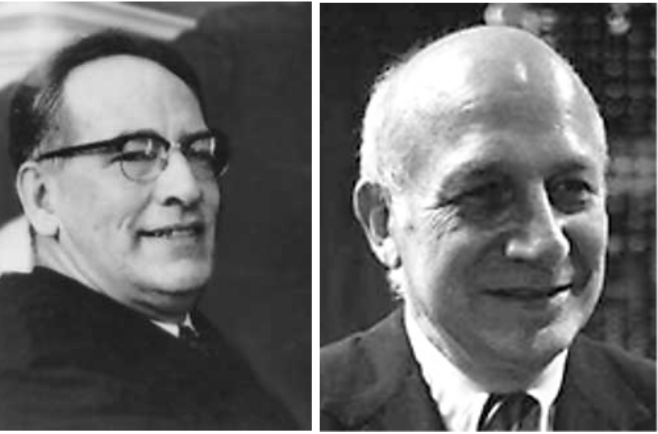
\includegraphics[scale = 0.31]{figs/Selection_01c2.png}
\end{figure}
Built ENIAC (Electronic Numerical Integrator and Computer), the first
electronic general-purpose computer during 1943-1945 at a cost of
\$468,000.
\end{frame}


\begin{frame}
\frametitle{Introduction}
\framesubtitle{Alan Mathison Turing\footnote{The Imitation Game: A 2014 Movie biographied on turing}}
\begin{figure}[!tbp]
\centering
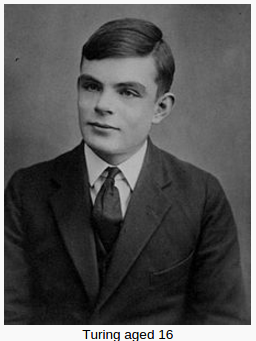
\includegraphics[scale = 0.35]{figs/alan.png}
\end{figure}
\begin{itemize}
\item {\bf Born}: 23 June 1912
\item Turing is widely considered to be the father of theoretical computer science and artificial intelligence
\item Famous for Breaking Enigma Machine Code
\item {\bf Died}: 7 June 1954 (aged 41)
\end{itemize}
\end{frame}

\begin{frame}
\frametitle{Turing Machine}
\begin{tikzpicture}
\tikzstyle{every path}=[very thick]

\edef\sizetape{0.7cm}
\tikzstyle{tmtape}=[draw,minimum size=\sizetape]
\tikzstyle{tmhead}=[arrow box,draw,minimum size=.5cm,arrow box
arrows={east:.25cm, west:0.25cm}]

%% Draw TM tape
\begin{scope}[start chain=1 going right,node distance=-0.15mm]
    \node [on chain=1,tmtape,draw=none] {$\ldots$};
    \node [on chain=1,tmtape] {};
    \node [on chain=1,tmtape] (input) {b};
    \node [on chain=1,tmtape] {b};
    \node [on chain=1,tmtape] {a};
    \node [on chain=1,tmtape] {a};
    \node [on chain=1,tmtape] {a};
    \node [on chain=1,tmtape] {a};
    \node [on chain=1,tmtape] {};
    \node [on chain=1,tmtape,draw=none] {$\ldots$};
    \node [on chain=1] {\textbf{\scriptsize{Input/Output Tape}}};
\end{scope}
%% Draw TM Finite Control
\begin{scope}
[shift={(3cm,-5cm)},start chain=circle placed {at=(-\tikzchaincount*60:1.5)}]
\foreach \i in {q_0,q_1,q_2,q_3,\ddots,q_n}
	\node [on chain] {$\i$};

% Arrow to current state
\node (center) {};
\draw[->] (center) -- (circle-2);

\node[rounded corners,draw=black,thick,fit=(circle-1) (circle-2) (circle-3) 
      (circle-4) (circle-5) (circle-6),
			label=below:\textbf{Finite Control}] (fsbox)
		{};
\end{scope}

%% Draw TM head below (input) tape cell
\node [tmhead,yshift=-.3cm] at (input.south) (head) {$q_1$};

%% Link Finite Control with Head
\path[->,draw] (fsbox.north) .. controls (4.5,-1) and (0,-2) .. node[right] 
			(headlinetext)
 			{} 
			(head.south);
\node[xshift=3cm] at (headlinetext)  
			{\begin{tabular}{c} 
				\textbf{Reading and Writing Head} \\  
				\textbf{(moves in both directions)} 
			 \end{tabular}};

\end{tikzpicture}
\end{frame}

\begin{frame}
\frametitle{History \\ {\large FORTRAN}}
\begin{figure}[!tbp]
\centering
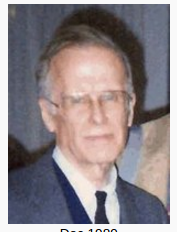
\includegraphics[scale = 0.35]{figs/Selection_007.png}
\end{figure}
\begin{itemize}
\item Inventor: John Backus
\item[\ding{45}]  FORTRAN, derived from Formula Translating System
\item It is a general-purpose, imperative programming language that is especially suited to numeric computation and scientific computing. Originally developed by IBM
\item First Appeared: 1957; 59 years ago
\end{itemize}
\end{frame}

\begin{frame}
\frametitle{History \\ {\large C++}}
\begin{figure}[!tbp]
\centering
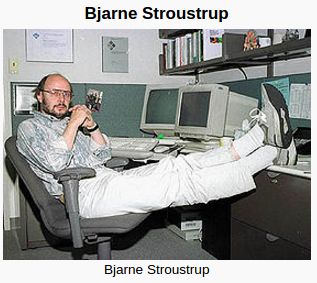
\includegraphics[scale = 0.35]{figs/cpr.png}
\end{figure}
\scriptsize{
\begin{itemize}
\item Inventor: Bjarne Stroustrup (at Bell Labs)
\item It is a general-purpose programming language. It has imperative, object-oriented and generic programming features, while also providing facilities for low-level memory manipulation
\item C++ is standardized by the International Organization for Standardization (ISO)
\item First Appeared: 1983; 33 years ago
\end{itemize}}
\end{frame}

\begin{frame}[shrink]%allowframebreaks]
\frametitle{Excellence of Human}
\framesubtitle{Equations: Changed The World}
\footnotesize{
 \resizebox{\linewidth}{!}{
%\begin{center}
\begin{tabular}{p{3.5cm} p{4.5cm} p{3cm}}
\\ \\ 
 \multicolumn{3}{c}{\textcolor{olive}{17 Equations That Changed The World}} \\ \\
 Pythagora.s Theorem&$a^2+b^2=c^2$&Pythagoras,530 BC\\
 Logarithms&$logxy=logx+logy$& John Napier, 1610\\
 Calculus &$\frac{df}{dt}=\lim_{h \to 0}\frac{f(t+h)-f(t)}{h}$& Newton, 1668\\
Law of Gravity   &$F=G\frac{m_1m_2}{r^2}$& Newton, 1687\\
Complex Identity&$i^2=-1$& Euler, 1750\\
Polyhedra Formula&$V-E+F=2$& Euler, 1751\\
Normal Distribution&$\phi(x)=\frac{1}{\sqrt{2\pi\rho}}e^\frac{(x-\mu)^2}{2\rho^2}$& C.F. Gauss, 1810\\
Wave Equation&$\frac{\partial^2u}{\partial t^2}=c^2\frac{\partial^2u}{\partial x^2}$& J. d'Almbert,1746\\
Fourier Transform&$f(\omega)=\int_{-\infty}^\infty f(x)e^{-2\pi ix\omega}dx$& J. Fourier, 1822\\
Navier-Stokes Equation&$\rho(\frac{\partial v}{\partial t}+v.\nabla v)=-\nabla p+\nabla .T+f$& C. Navier, G. Stokes, 1845\\
Maxwell's Equations& {\tiny{\begin{tabular}{c c}
$\nabla  E=\frac{\rho}{\epsilon 0}$ & $\nabla .H=0$ \\ 
$\nabla \times E=-\frac{1}{c}\frac{\partial H}{\partial t}$ & $\nabla \times H=\frac{1}{c}\frac{\partial E}{\partial t}$
\end{tabular}}}& J.C. Maxwell, 1865\\
Second Law of Thermosynamics &$dS\ge0$ & L. Boltzmann, 1874\\
Relativity & $E=mc^2$&Einstein, 1905\\
Schrodinger's Equation &$i\hslash\frac{\partial}{\partial t}\Psi=H\Psi$&E. Schrodinger, 1927\\
Information Theory &$H=-\sum p(x)logp(x)$&C. Shannon, 1949 \\
Chaos Theory &$x_{t+1}=kx_t(1-x_t)$& Robert May,1975\\
Black-Scholes\\ Equation&$\frac{1}{2}\sigma^2S^2\frac{\partial^2V}{\partial S^2}+rS\frac{\partial V}{\partial S}+\frac{\partial V}{\partial t}-rV=0$&F. Black, M. Scholes, 1990\\
\end{tabular}}}
%\end{center}}}
\end{frame}









\begin{frame}
\frametitle{Introduction \\ {\large Modern programming}}
Whatever the approach to development may be, the final program must satisfy some fundamental properties. The following properties are among the most important
\begin{itemize}
\item[\ding{90}] Reliability
\item[\ding{90}] Robustness
\item[\ding{90}] Usability
\item[\ding{90}] Portability
\item[\ding{90}] Maintainability
\item[\ding{90}] Efficiency/performance
\end{itemize}
\end{frame}

\begin{frame}
\frametitle{History \\ {\large 4GL}}
Some fourth generation programming language
\begin{itemize}
\item Matlab/Simulink
\item LabVIEW
\item Python
\item Wolfram
\item Unix Shell
\end{itemize}
\end{frame}

\subsection{Matlab}
\begin{frame}
\frametitle{Introduction\\ {\large Matlab}}
\begin{figure}[!tbp]
\centering
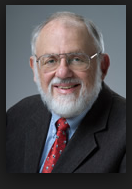
\includegraphics[scale = 0.5]{figs/matl.png}
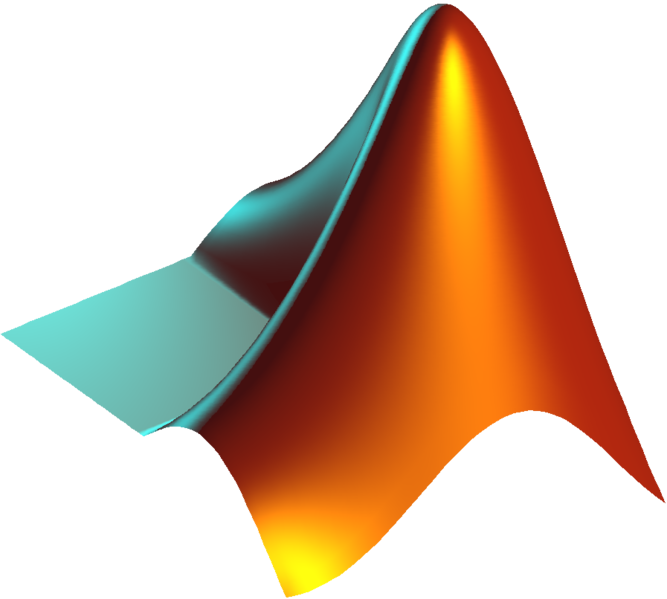
\includegraphics[scale = 0.08]{figs/Selection_035.png}
\end{figure}
\small{
\begin{itemize}
\item Initial Release: 1984; 32 years ago
\item MATLAB is a multi-paradigm numerical computing environment and fourth-generation programming language
\item Widely Used for Academic, Research \& Development
\item Cross-Platform Software
\item Latest Stable Release: Matlab R2015b
\end{itemize}}
\end{frame}

\subsection{LabVIEW}
\begin{frame}
\frametitle{Introduction\\ {\large LabVIEW}}
\begin{figure}[!tbp]
\centering

\includegraphics[scale = 0.5]{figs/fg.png}
\end{figure}
\begin{itemize}
\item Initial Release: 1983; 33 years ago
\item LabVIEW (short for Laboratory Virtual Instrument Engineering Workbench) is a system-design platform and development environment for a visual programming language from National Instruments
\item The graphical language is named "G" used by LabVIEW
\item Cross-Platform Software
\item Latest Stable Release: 2015/ August 2015
\end{itemize}
\end{frame}








%%%%%%%%%%%%%%%%%%%%%%%%
\subsection{Basic Math}
\begin{frame}
\frametitle{Calculus \\ {\large Integration by parts}}
\begin{figure}[!tbp]
\centering
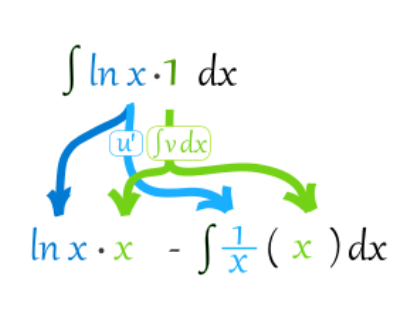
\includegraphics[scale = 0.35]{figs/Selection_011.png}
\footnote{\href{http://www.mathsisfun.com/calculus/integration-by-parts.html}{\beamergotobutton{Link}}}
\end{figure}
\end{frame}
\begin{frame}
\frametitle{Linear Algebra \\ {\large Partial fraction expansion}}
\begin{figure}[!tbp]
\centering
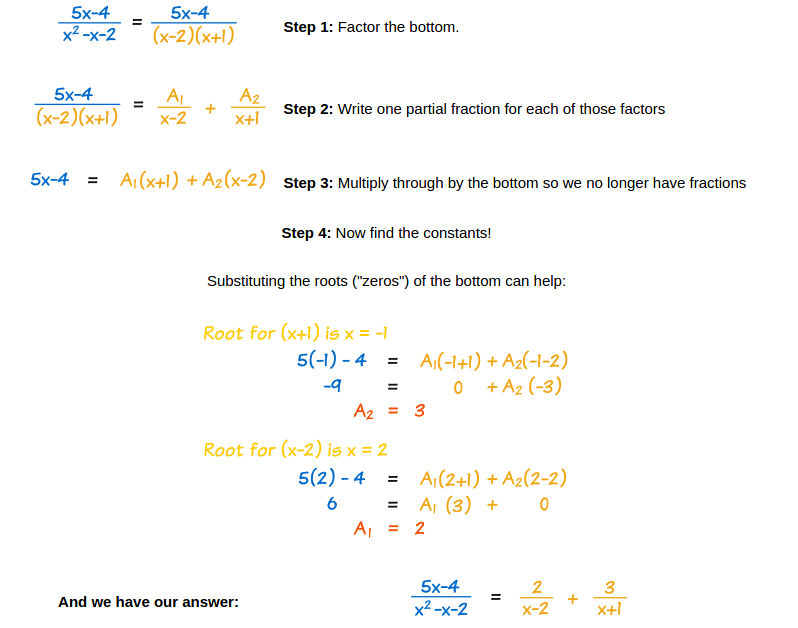
\includegraphics[scale = 0.3]{figs/Selection_012.png}
\footnote{\href{http://www.mathsisfun.com/calculus/integration-by-parts.html}{\beamergotobutton{Link}}}
\end{figure}
\end{frame}
\begin{frame}
\frametitle{Linear Algebra \\ {\large Determinants}}
Here's an easy illustration that shows why the \textcolor{blue}{determinant} of a matrix with \textcolor{blue}{linear dependent} rows is 0

$$M=\begin{bmatrix}
    a       & b \\
    2a     &2b \\
\end{bmatrix}$$
$$\Rightarrow |M|=a(2b) - 2b(a)=0$$  \\
Let's look at a 3x3 example.
\end{frame}

\begin{frame}
\frametitle{Linear Algebra \\ {\large Determinants}}
$M=\begin{bmatrix}
    a       & b  &c\\
    2a     &2b &c\\
    d       &e   &f\\
\end{bmatrix}$ \\
$\Rightarrow |M|=a(2bf-2ce) - b(2af-2cd)+c(2ae-2bd)=0$ \\
Let's change the order of rows \\
$M=\begin{bmatrix}
 d       &e   &f\\   
 a       & b  &c\\
    2a     &2b &c\\
\end{bmatrix}$ \\
$\Rightarrow |M|=d(2bc - 2bc) - e(2ac - 2ac) + f (2ab - 2ab)=0$
Let's change the order of rows again\\
$M=\begin{bmatrix}
 d       &e   &f\\ 
 2a     &2b &c\\  
 a       & b  &c\\
\end{bmatrix}$ \\
$\Rightarrow |M|=a(2ce - 2bf ) - b(2dc - 2af ) + c(2db - 2ae)=0$ \\
In other words, if we have dependent rows, then the determinant of the
matrix is 0
\end{frame}
  
\begin{frame}
\frametitle{Linear Algebra \\ {\large Adjoint of matrix}}
\begin{figure}[!tbp]
\centering
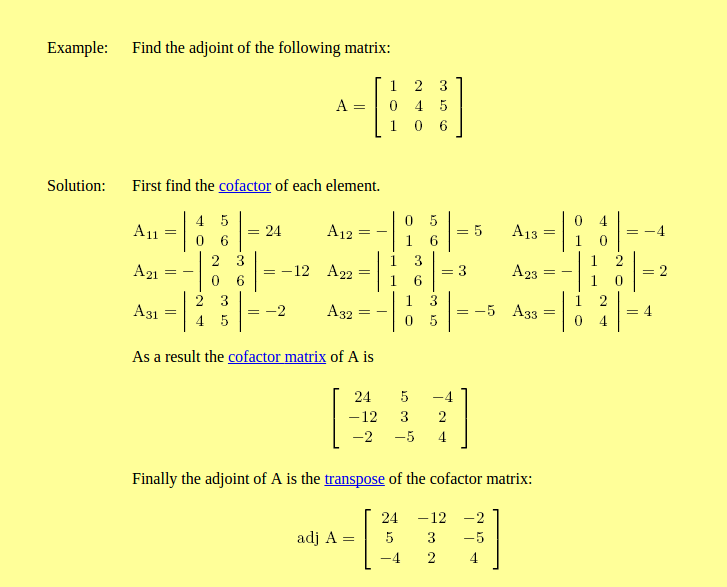
\includegraphics[scale = 0.35]{figs/Selection_013.png}
\footnote{\href{http://www.mathwords.com/a/adjoint.htm}{\beamergotobutton{Link}}}
\end{figure}
\end{frame}

\begin{frame}
\frametitle{Linear Algebra \\ {\large Inverse of matrix}}
\begin{center}
$A^{-1}=\frac{1}{|A|}$(Adjoint of A)
\end{center}
\end{frame}
\subsection{Laplace}
\begin{frame}
\frametitle{Laplace Transform \\ {\large Tables}}
\begin{figure}[!tbp]
\centering
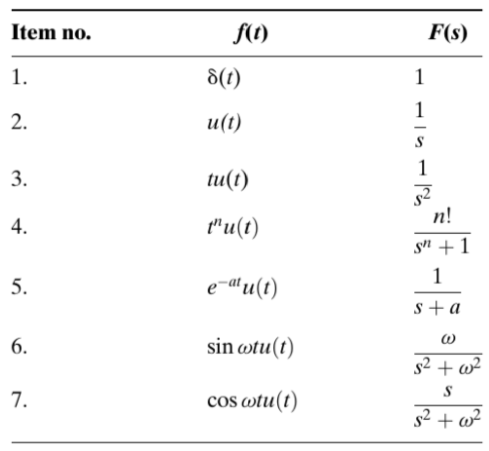
\includegraphics[scale = 0.46]{figs/Selection_014.png}
\end{figure}
\end{frame}

\begin{frame}
\frametitle{Laplace Transform \\ {\large Tables}}
\begin{figure}[!tbp]
\centering
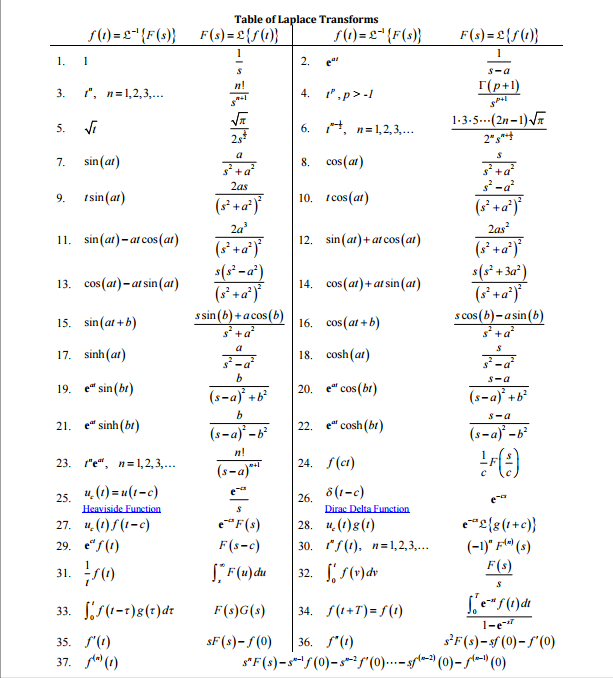
\includegraphics[scale = 0.3]{figs/Selection_015.png}
\footnote{\href{http://tutorial.math.lamar.edu/pdf/Laplace_Table.pdf}{\beamergotobutton{Link}}}
\end{figure}
\end{frame}

\begin{frame}
\frametitle{Laplace Transform \\ {\large Tables}}
\begin{figure}[!tbp]
\centering
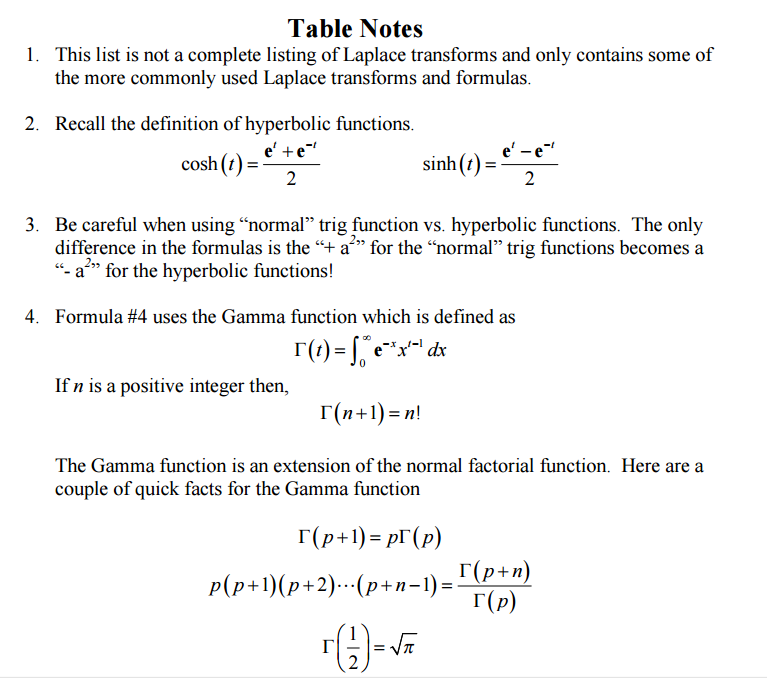
\includegraphics[scale = 0.3]{figs/Selection_018.png}
\footnote{\href{http://tutorial.math.lamar.edu/pdf/Laplace_Table.pdf}{\beamergotobutton{Link}}}
\end{figure}
\end{frame}



\begin{frame}
\frametitle{Parabolic Graph}
\pagestyle{empty}
\begin{tikzpicture}[scale=1.8]
  \shade[top color=blue,bottom color=gray!50] 
      (0,0) parabola (1.5,2.25) |- (0,0);
  \draw (1.07cm,2pt) node[above] 
      {\scriptsize $\displaystyle\int_0^{3/2} \!\!x^2\mathrm{d}x$};

  \draw[style=help lines] (0,0) grid (3.9,3.9)
       [step=0.25cm]      (1,2) grid +(1,1);

  \draw[->] (-0.2,0) -- (4,0) node[right] {$x$};
  \draw[->] (0,-0.2) -- (0,4) node[above] {$f(x)$};

  \foreach \x/\xtext in {1/1, 1.5/1\frac{1}{2}, 2/2, 3/3}
    \draw[shift={(\x,0)}] (0pt,2pt) -- (0pt,-2pt) node[below] {$\xtext$};

  \foreach \y/\ytext in {1/1, 2/2, 2.25/2\frac{1}{4}, 3/3}
    \draw[shift={(0,\y)}] (2pt,0pt) -- (-2pt,0pt) node[left] {$\ytext$};

  \draw (-.5,.25) parabola bend (0,0) (2,4) node[below right] {$x^2$};
\end{tikzpicture}
\end{frame}



\begin{frame}
\frametitle{Fast Fourier Transform}
\tiny{
\begin{tikzpicture}[transform shape]
  %the multiplication with floats is not possible. Thus I split the loop in two.
  \foreach \number in {1,...,8}{
      % Computer angle:
        \mycount=\number
        \advance\mycount by -1
  \multiply\mycount by 45
        \advance\mycount by 0
      \node[draw,circle,inner sep=0.25cm] (N-\number) at (\the\mycount:5.4cm) {};
    }
  \foreach \number in {9,...,16}{
      % Computer angle:
        \mycount=\number
        \advance\mycount by -1
  \multiply\mycount by 45
        \advance\mycount by 22.5
      \node[draw,circle,inner sep=0.25cm] (N-\number) at (\the\mycount:5.4cm) {};
    }
  \foreach \number in {1,...,15}{
        \mycount=\number
        \advance\mycount by 1
  \foreach \numbera in {\the\mycount,...,16}{
    \path (N-\number) edge[->,bend right=3] (N-\numbera)  edge[<-,bend
      left=3] (N-\numbera);
  }
}
\end{tikzpicture}
}
\end{frame}


\begin{frame}
\frametitle{Flow Chart}
\tikzstyle{startstop} = [rectangle, rounded corners, minimum width=1.8cm, minimum height=0.5cm,text centered, draw=black, fill=red!30]
\tikzstyle{io} = [trapezium, trapezium left angle=70, trapezium right angle=110, minimum width=1.8cm, minimum height=0.5cm, text centered, draw=black, fill=blue!30]
\tikzstyle{process} = [rectangle, minimum width=1.8cm, minimum height=0.6cm, text centered, draw=black, fill=orange!30]
\tikzstyle{decision} = [diamond, minimum width=1.2cm, minimum height=0.3cm, text centered, draw=black, fill=green!30]
\tikzstyle{arrow} = [thick,->,>=stealth]
\begin{center}
\tiny{
\begin{tikzpicture}[node distance=1.3cm]
\node (start) [startstop] {Start};
\node (in1) [io, below of=start] {Input};
\node (pro1) [process, below of=in1] {Process 1};
\node (dec1) [decision, below of=pro1] {Decision 1};
\node (pro2a) [process, below of=dec1, yshift=-0.15cm] {Process 2a};
\node (pro2b) [process, right of=dec1, xshift=2cm] {Process 2b};
\node (out1) [io, below of=pro2a] {Output};
\node (stop) [startstop, below of=out1] {Stop};
\draw [arrow] (start) -- (in1);
\draw [arrow] (in1) -- (pro1);
\draw [arrow] (pro1) -- (dec1);
\draw [arrow] (dec1) -- (pro2a);
\draw [arrow] (dec1) -- (pro2b);;
\draw [arrow] (dec1) -- node[anchor=east] {yes} (pro2a);
\draw [arrow] (dec1) -- node[anchor=south] {no} (pro2b);
\draw [arrow] (pro2a) -- (out1);
\draw [arrow] (out1) -- (stop);
\draw [arrow] (pro2b) |- (pro1);
\end{tikzpicture}}
\end{center}
\end{frame}


\begin{frame}[shrink]
\frametitle{Flow Chart}
\pagestyle{empty}

\centering
% Define block styles
\tikzstyle{decision} = [diamond, draw, fill=blue!20, 
    text width=4.5em, text badly centered, node distance=3cm, inner sep=0pt]
\tikzstyle{block} = [rectangle, draw, fill=blue!20, 
    text width=5em, text centered, rounded corners, minimum height=4em]
\tikzstyle{line} = [draw, -latex']
\tikzstyle{cloud} = [draw, ellipse,fill=red!20, node distance=3cm,
    minimum height=2em]
    
\begin{tikzpicture}[node distance = 2cm, auto]
    % Place nodes
    \node [block] (init) {initialize model};
    \node [cloud, left of=init] (expert) {expert};
    \node [cloud, right of=init] (system) {system};
    \node [block, below of=init] (identify) {identify candidate models};
    \node [block, below of=identify] (evaluate) {evaluate candidate models};
    \node [block, left of=evaluate, node distance=3cm] (update) {update model};
    \node [decision, below of=evaluate] (decide) {is best candidate better?};
    \node [block, below of=decide, node distance=3cm] (stop) {stop};
    % Draw edges
    \path [line] (init) -- (identify);
    \path [line] (identify) -- (evaluate);
    \path [line] (evaluate) -- (decide);
    \path [line] (decide) -| node [near start] {yes} (update);
    \path [line] (update) |- (identify);
    \path [line] (decide) -- node {no}(stop);
    \path [line,dashed] (expert) -- (init);
    \path [line,dashed] (system) -- (init);
    \path [line,dashed] (system) |- (evaluate);
\end{tikzpicture}

\end{frame}






\section{Overview}
\begin{frame}
\frametitle{Laplace Transform \\ {\large Plot of simple first order equation}} 
Let $H(s) = \frac{1}{s+10}$,We've plotted the magnitude of H(s) below, i.e., $\vert H(s) \vert$. Other
possible 3D plots are $\angle$ H(s), Re(H(s)) and Im(H(s)) respectively. Notice that $|H(s)|$ goes to $\infty$
at the pole s = -10.
\begin{figure}[!tbp]
\centering
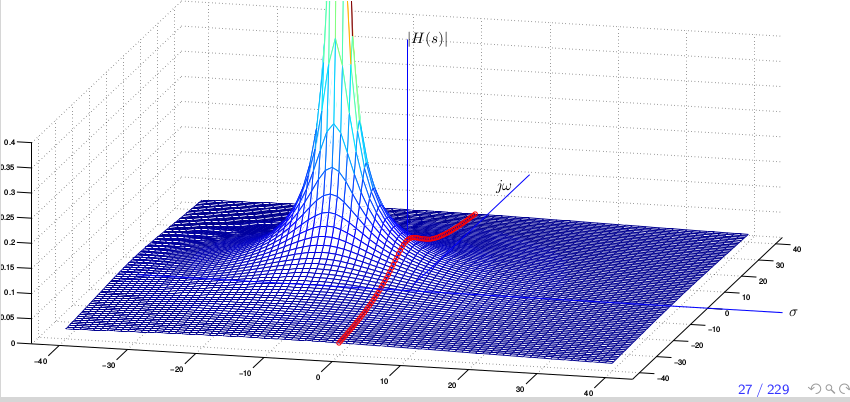
\includegraphics[scale = 0.4]{figs/Selection_016.png}
\end{figure}
\end{frame}





\begin{frame}
\frametitle{Laplace Transform}
\framesubtitle{3-D code for Transfer functions \attachfile{codes/qazie.m}}

\begin{tcolorbox}[title=  ,width=9.85 cm]
\lstinputlisting{codes/qazie.m}
\end{tcolorbox}
\end{frame}

%%%%%%%%%%%%%%%%%%%%

\begin{frame}
\frametitle{Laplace Transform \\ {\large Plot of Second order equation}}
Let $H(s) = \frac{s+5}{(s+10)(s-5)}$. We've plotted the magnitude of H(s) below, i.e., $|H(s)|$. Other
possible 3D plots are $\angle$H(s), Re(H(s)) and Im(H(s)), respectively. Notice that $|H(s)|$ goes to $\infty$ at the pole s = -10 and 5 while it converges to down at the zero s=-5. 
 \begin{beamerboxesrounded}[shadow=true]{}
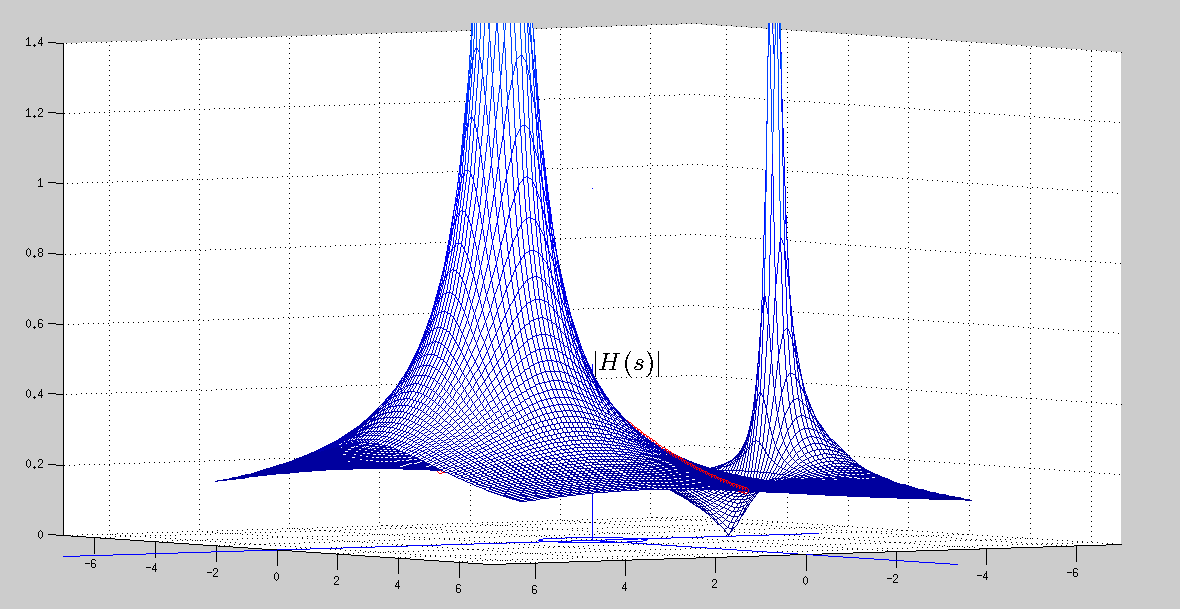
\includegraphics[width=100mm]{figs/Selection_004.png}
\end{beamerboxesrounded}

\end{frame}

\begin{frame}
\frametitle{Laplace Transform \\ {\small Laplace Transform of integration and derivative}}
For more details on how the Laplace transform for
integration is 1/s and Laplace transform for derivative
is s then see 
\begin{beamerboxesrounded}[shadow=true]{}
\url{http://www2.kau.se/yourshes/AB2 8.pdf}
\end{beamerboxesrounded}
\end{frame}

\begin{frame}
\frametitle{Control Systems \\ {\small FREQUENCY (Continous) and Time}} 
\begin{figure}[!tbp]
\centering
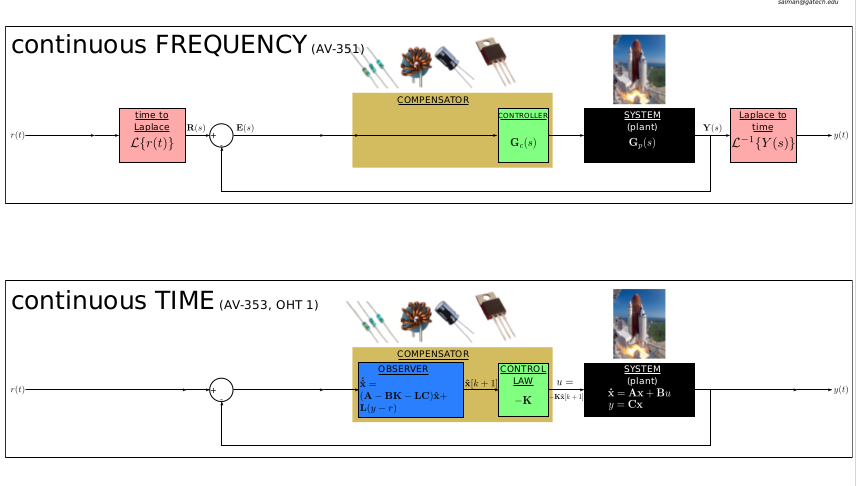
\includegraphics[scale = 0.35]{figs/Selection_019.png}
\end{figure}
\end{frame}

\begin{frame}
\frametitle{Control Systems \\ {\large Introduction}} 
Among mechanistic systems, we are interested in linear
systems. Here are some examples:
\begin{enumerate}
  \item Filters (analog and digital
  \item Control sysytems
\begin{itemize}
\item A \textcolor{blue}{control system} is an interconnection of
components forming a system configuration that
will provide a desired system response
\item An \textcolor{blue}{open loop control system} utilizes an actuating
device to control the process directly without using
feedback uses a controller and an actuator to
obtain the desired response
\item A \textcolor{blue}{closed loop control system} uses a measurement
of the output and feedback of this signal to
compare it with the desired output (reference or
command)
\end{itemize}
\end{enumerate}
\end{frame}

\begin{frame}
\frametitle{Control Systems \\ {\large Introduction}} 
\begin{itemize}
\item To understand and control complex systems, one
must obtain quantitative \textcolor{blue}{mathematical models} of
these systems
\item It is therefore necessary to analyze the relationships
between the system variables and to obtain a
mathematical model
\item Because the systems under consideration are
dynamic in nature, the descriptive equations are
usually  \textcolor{blue}{differential equations}
\item Furthermore, if these equations are linear or can be
linearized, then the \textcolor{blue}{Laplace Transform} can be
used to simplify the method of solution
\end{itemize}
\end{frame}

\begin{frame}
\frametitle{Control Systems \\ {\large Introduction}} 
Control system analysis and design focuses on three
things:
\begin{enumerate}
\item transient response
\item stability
\item steady state errors
\end{enumerate}
For this, the equation (model), impulse response and
step response are studied. Other important parameters
are sensitivity/robustness and optimality.
Control system design entails tradeoffs between desired
transient response, steady-state error and the
requirement that the system be stable.
\label{contents}
\end{frame}

\begin{frame}
\frametitle{Control Systems \\ {\large Analysis}} 
The analysis of control systems can be done in the following nine ways:
\begin{enumerate}
\item equation
\item poles/zeros/controllability/observability
\item stability
\item impulse response
\item step response
\item steady-state response
\item transient response
\item sensitivity
\item optimality
\end{enumerate}
The design of control systems can be done in the following ways:
\begin{enumerate}
\item Pole placement (PID in frequency and time, state feedback in
time)
\end{enumerate}
\hyperlink{contents}{\beamergotobutton{Back to immediate slide}}
\end{frame}

\section{Signal and Systems}

\begin{frame}
\frametitle{Linear algebra}
\framesubtitle{Eigen-decomposition}
\begin{tcolorbox}[width=\textwidth,colback={mygray!20},title={},outer arc=0.01mm,colupper=black]    
A: NxN square matrix with \\
N linearly independent eigenvectors \\
\begin{tabular}{c c}
\colorbox{red!85}{$A=S\wedge S^{-1}$} & \textcolor{blue}{S: eigen vectors in the columns} \\
\textcolor{blue}{if A is symmetric} & \textcolor{blue}{$\wedge$: Diagonal eigen value matrix}
\end{tabular}
\end{tcolorbox} 

\begin{tcolorbox}[width=\textwidth,colback={mygray!20},title={},outer arc=0.01mm,colupper=black]   
{\tiny{ 
\begin{tabular}{c c c}
\quad & \textcolor{blue}{the eigenvectors}  &  \textcolor{blue}{Q: orthonormal}  \\
\quad & \textcolor{blue}{are orthonormal} &  \textcolor{blue}{eigenvectors in the columns} \\
\end{tabular}}}
\begin{tabular}{c c}
$A=Q\wedge Q^{-1}=Q\wedge Q^{T}$ &\hfill \\
\end{tabular}
\end{tcolorbox} 

\begin{tcolorbox}[width=\textwidth,colback={mygray!20},title={},outer arc=0.01mm,colupper=black]   
 \textcolor{blue}{the eigenvalues are real}
\end{tcolorbox}
\begin{center}
 \textcolor{blue}{all matrices are NxN}
\end{center}
\end{frame}

\begin{frame}
\frametitle{Linear algebra}
\framesubtitle{SVD}
\begin{figure}[!tbp]
\centering
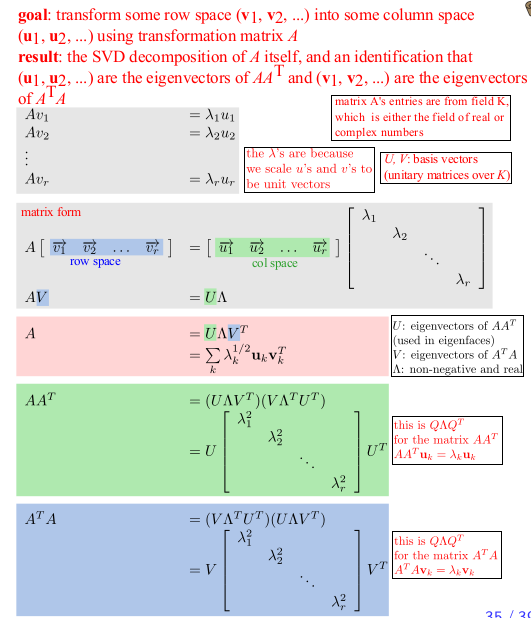
\includegraphics[scale = 0.35,keepaspectratio]{figs/svd.png}
\end{figure}
\end{frame}

\begin{frame}
\frametitle{Linear algebra}
\framesubtitle{SVD (example)}
\begin{figure}[!tbp]
\centering
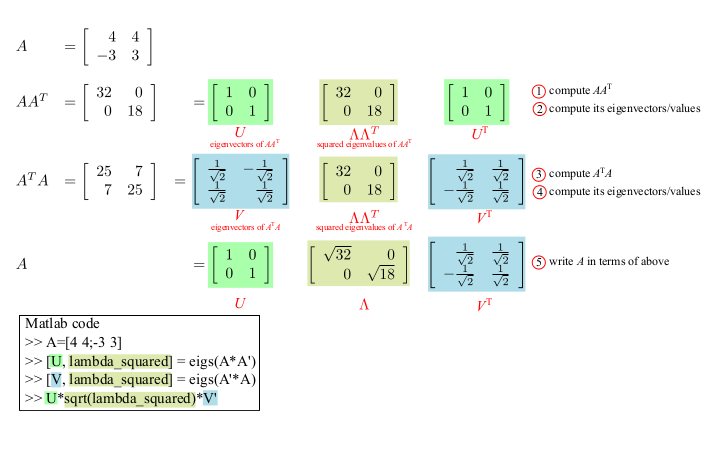
\includegraphics[scale = 0.4,keepaspectratio]{figs/svd1.png}
\end{figure}
\end{frame}



\subsection{Matrix reconstruction}
\begin{frame}
\frametitle{Linear Algebra}
\framesubtitle{SVD: successive matrix reconstruction}
\small{
\begin{itemize}
\item Z = sin(xy )
\item Original matrix size: 63$\times$63
\begin{itemize}
\item[\ding{44}] x and y axes, 0 : 0.1 : 2$\pi$
\end{itemize}
\item Max N: 63
\end{itemize}}
\begin{figure}[!htb]
\centering
\includegraphics [width=2.7in]{figs/abc_01.eps}
\end{figure}
\end{frame}















\begin{frame}
\frametitle{Linear Algebra}
\framesubtitle{SVD: successive matrix reconstruction {\tiny cont.}}
\small{
\begin{center}
\begin{align*}
Z &= sin(xy) \\
  &= \lambda_k{\bf u}_k {\bf v}_k^T
\end{align*} 
\end{center}}
\begin{figure}[!htb]
\centering
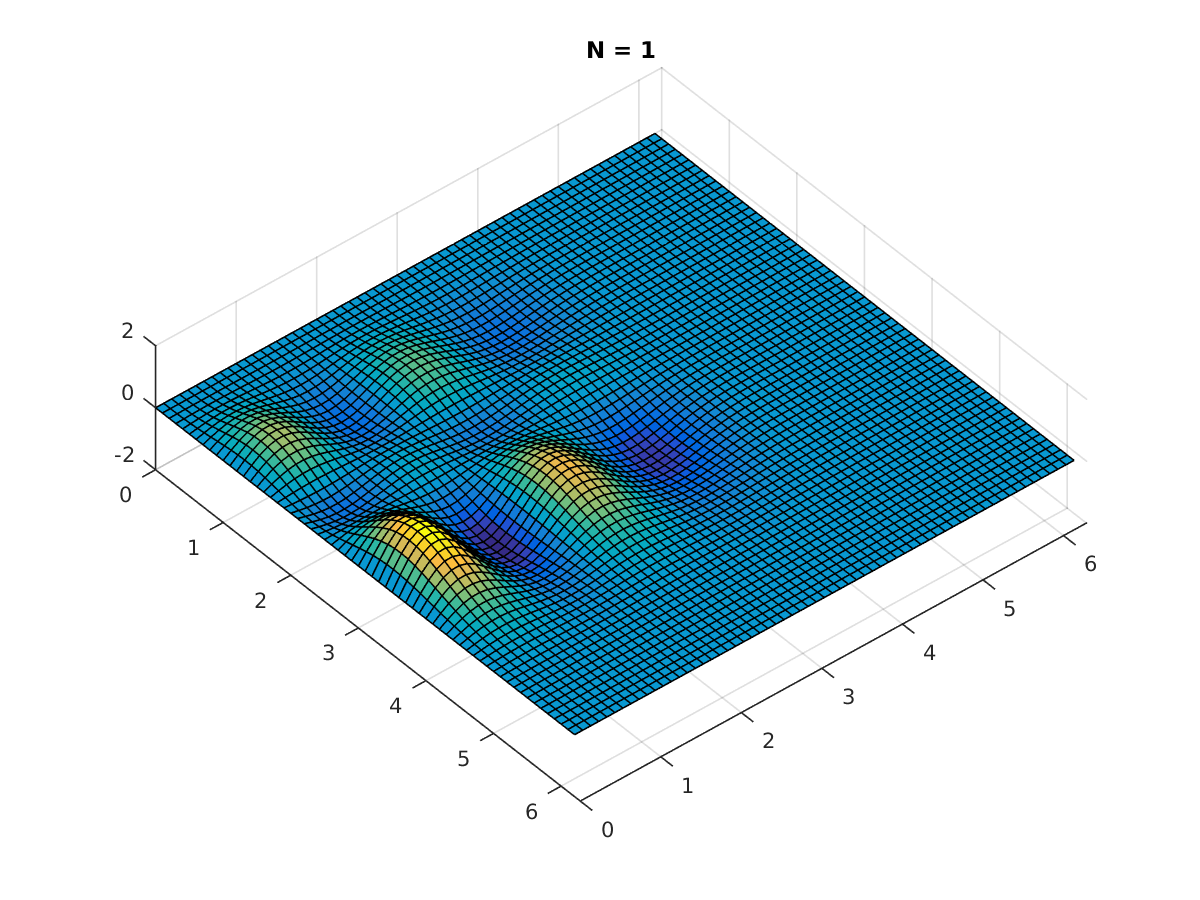
\includegraphics [scale=0.415]{as/a1.png}
\end{figure}
\end{frame}


\begin{frame}
\frametitle{Linear Algebra}
\framesubtitle{SVD: successive matrix reconstruction {\tiny cont.}}
\small{ 
\begin{center}
\begin{align*}
Z &= sin(xy) \\
  &= \lambda_k{\bf u}_k {\bf v}_k^T
\end{align*}
\end{center}}
\begin{figure}[!htb]
\centering
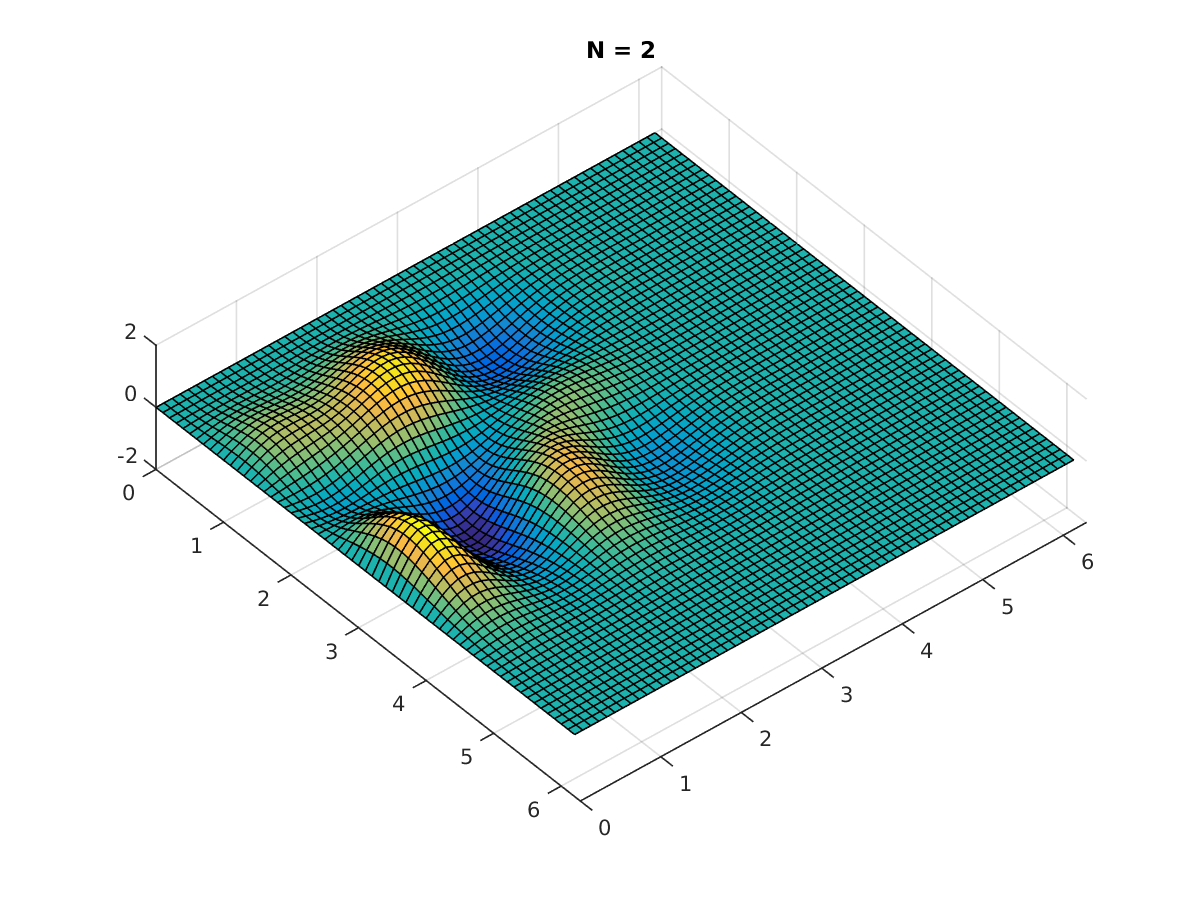
\includegraphics [scale=0.415]{as/a2.png}
\end{figure}
\end{frame}


\begin{frame}
\frametitle{Linear Algebra}
\framesubtitle{SVD: successive matrix reconstruction {\tiny cont.}}
\small{
\begin{center}
\begin{align*}
Z &= sin(xy) \\
  &= \lambda_k{\bf u}_k {\bf v}_k^T
\end{align*}
\end{center}}
\begin{figure}[!htb]
\centering
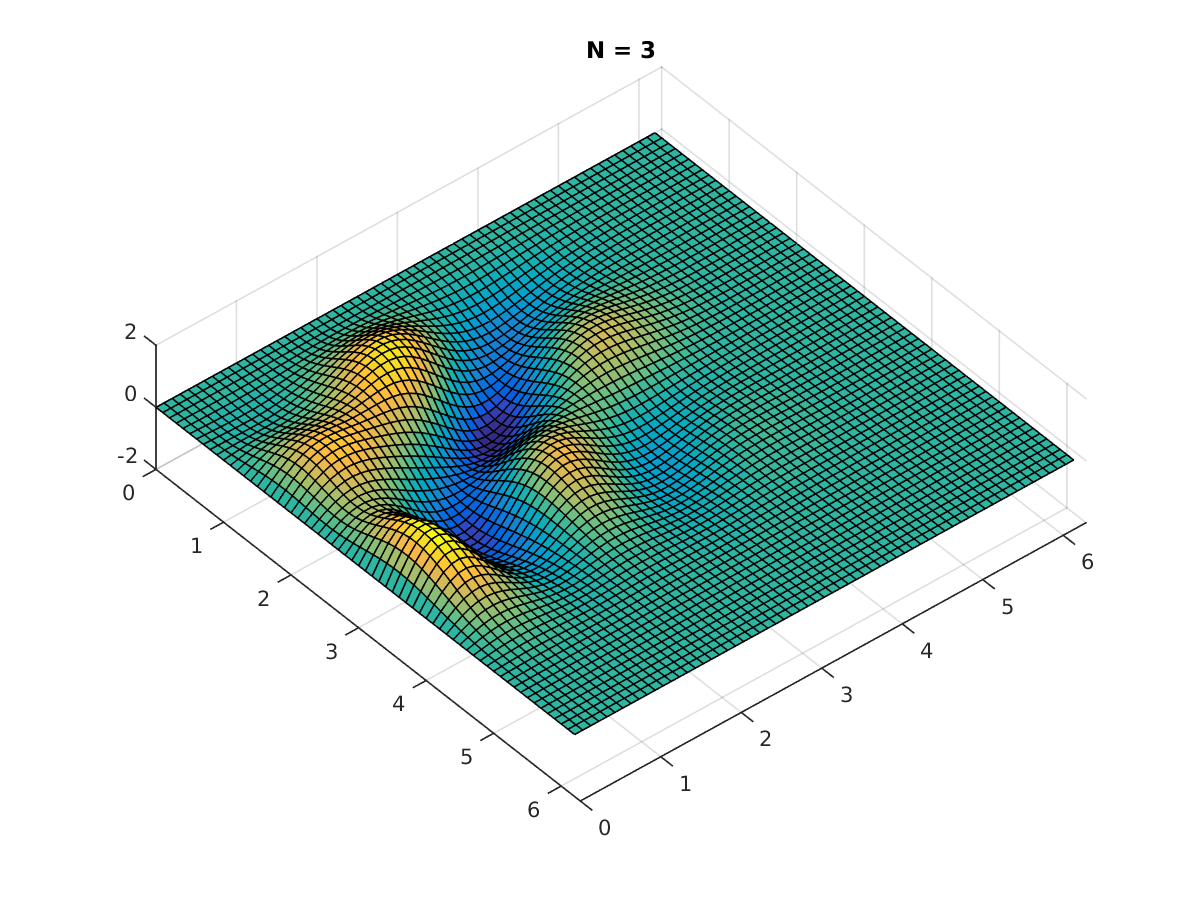
\includegraphics [scale=0.415]{as/a3.png}
\end{figure}
\end{frame}

\begin{frame}
\frametitle{Linear Algebra}
\framesubtitle{SVD: successive matrix reconstruction {\tiny cont.}} 
\small{
\begin{center}
\begin{align*}
Z &= sin(xy) \\
  &= \lambda_k{\bf u}_k {\bf v}_k^T
\end{align*}
\end{center}}
\begin{figure}[!htb]
\centering
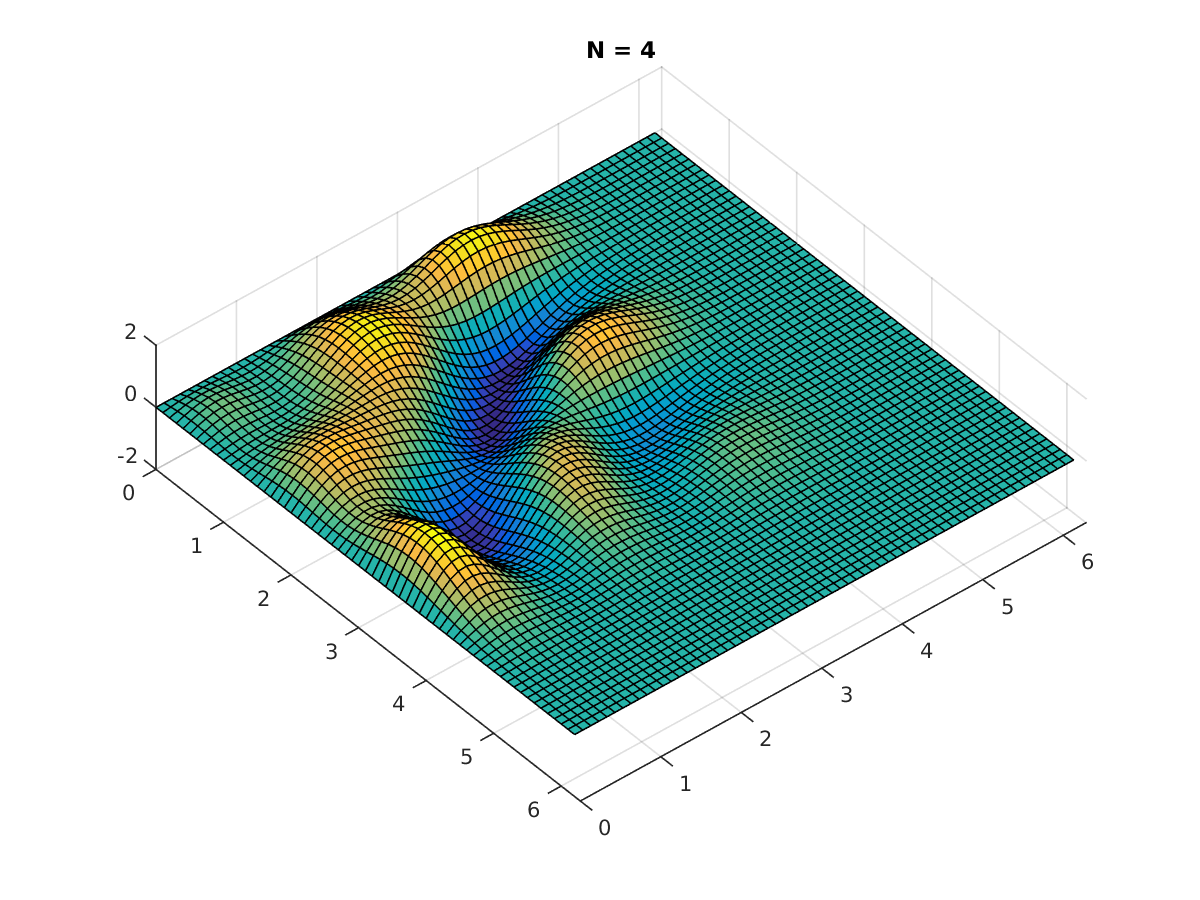
\includegraphics [scale=0.415]{as/a4.png}
\end{figure}
\end{frame}


\begin{frame}
\frametitle{Linear Algebra}
\framesubtitle{SVD: successive matrix reconstruction {\tiny cont.}} 
\small{
\begin{center}
\begin{align*}
Z &= sin(xy) \\
  &= \lambda_k{\bf u}_k {\bf v}_k^T
\end{align*}
\end{center}}
\begin{figure}[!htb]
\centering
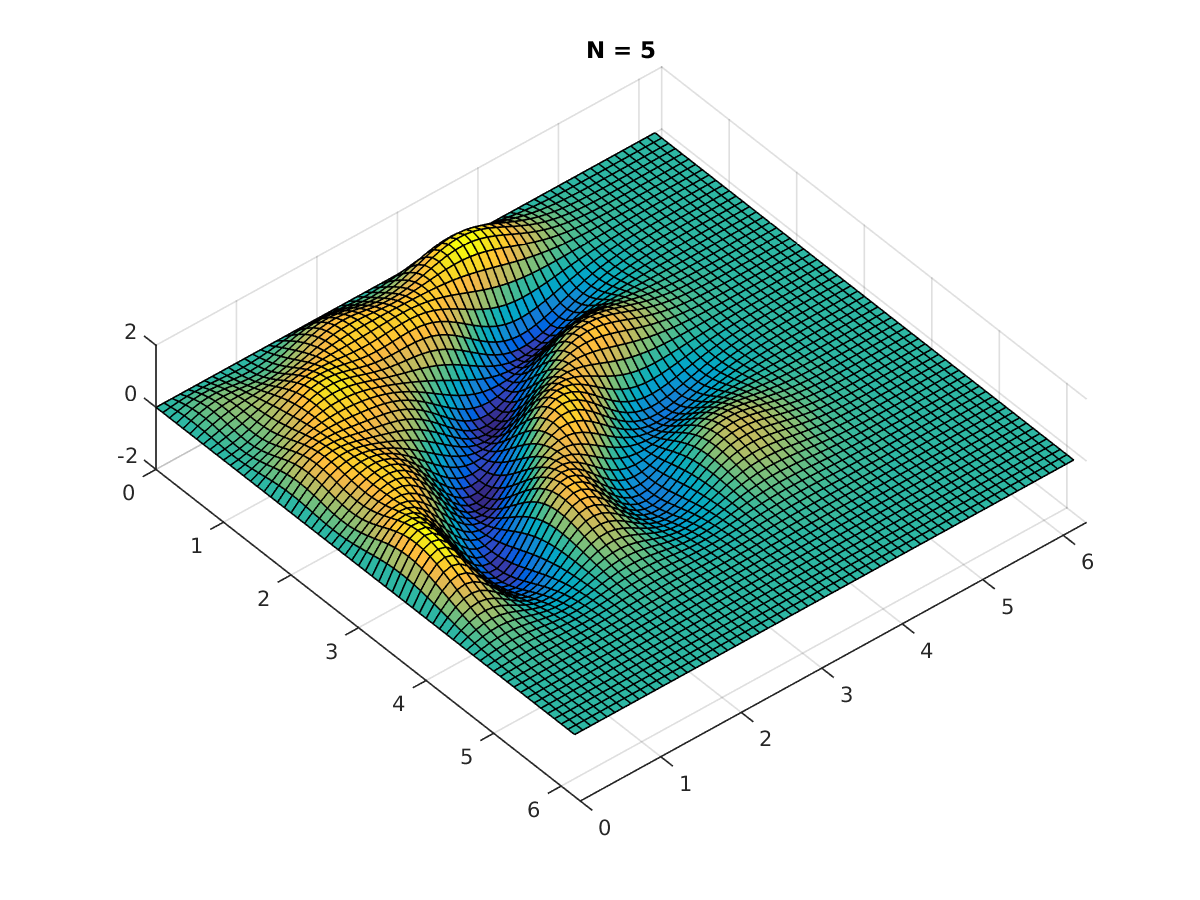
\includegraphics [scale=0.415]{as/a5.png}
\end{figure}
\end{frame}

\begin{frame}
\frametitle{Linear Algebra}
\framesubtitle{SVD: successive matrix reconstruction {\tiny cont.}} 
\small{
\begin{center}
\begin{align*}
Z &= sin(xy) \\
  &= \lambda_k{\bf u}_k {\bf v}_k^T
\end{align*}
\end{center}}
\begin{figure}[!htb]
\centering
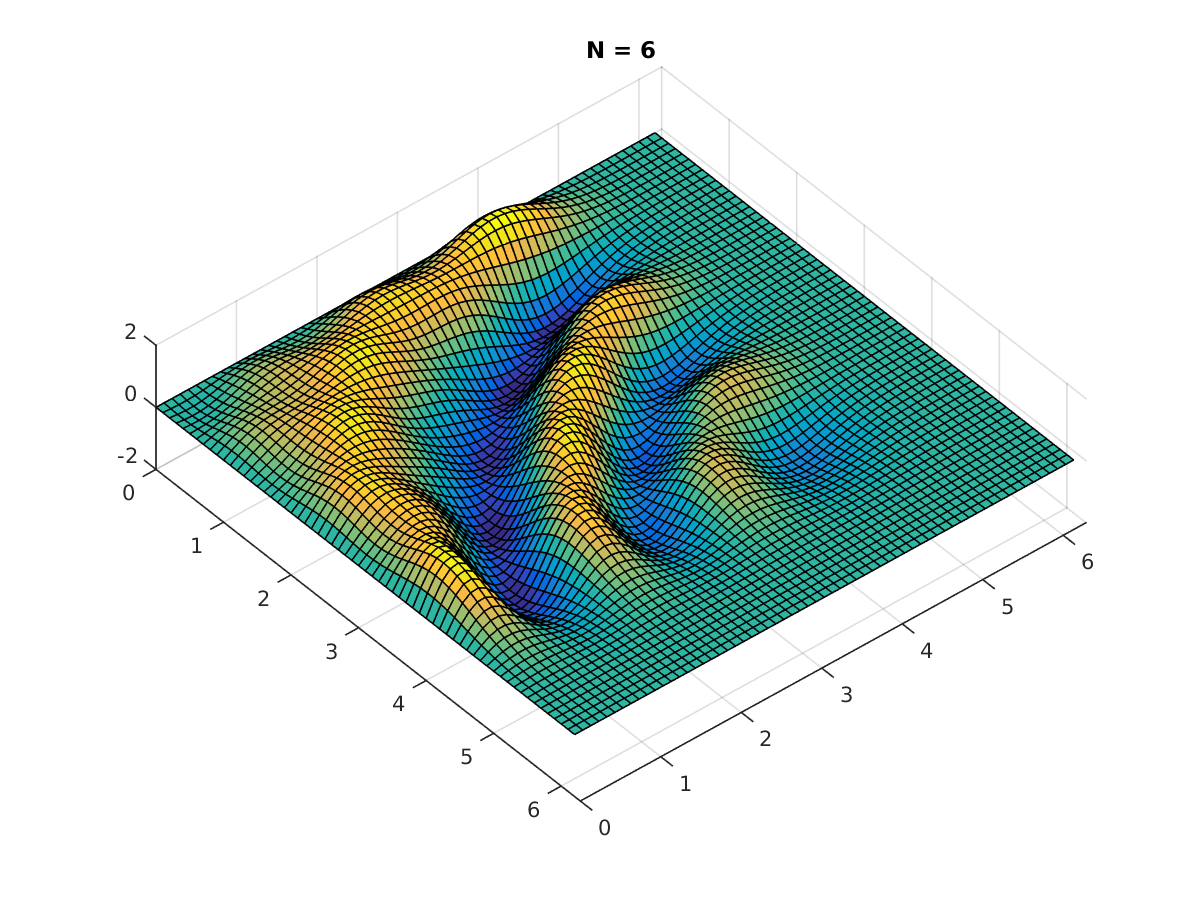
\includegraphics [scale=0.415]{as/a6.png}
\end{figure}
\end{frame}

\begin{frame}
\frametitle{Linear Algebra}
\framesubtitle{SVD: successive matrix reconstruction {\tiny cont.}} 
\small{
\begin{center}
\begin{align*}
Z &= sin(xy) \\
  &= \lambda_k{\bf u}_k {\bf v}_k^T
\end{align*}
\end{center}}
\begin{figure}[!htb]
\centering
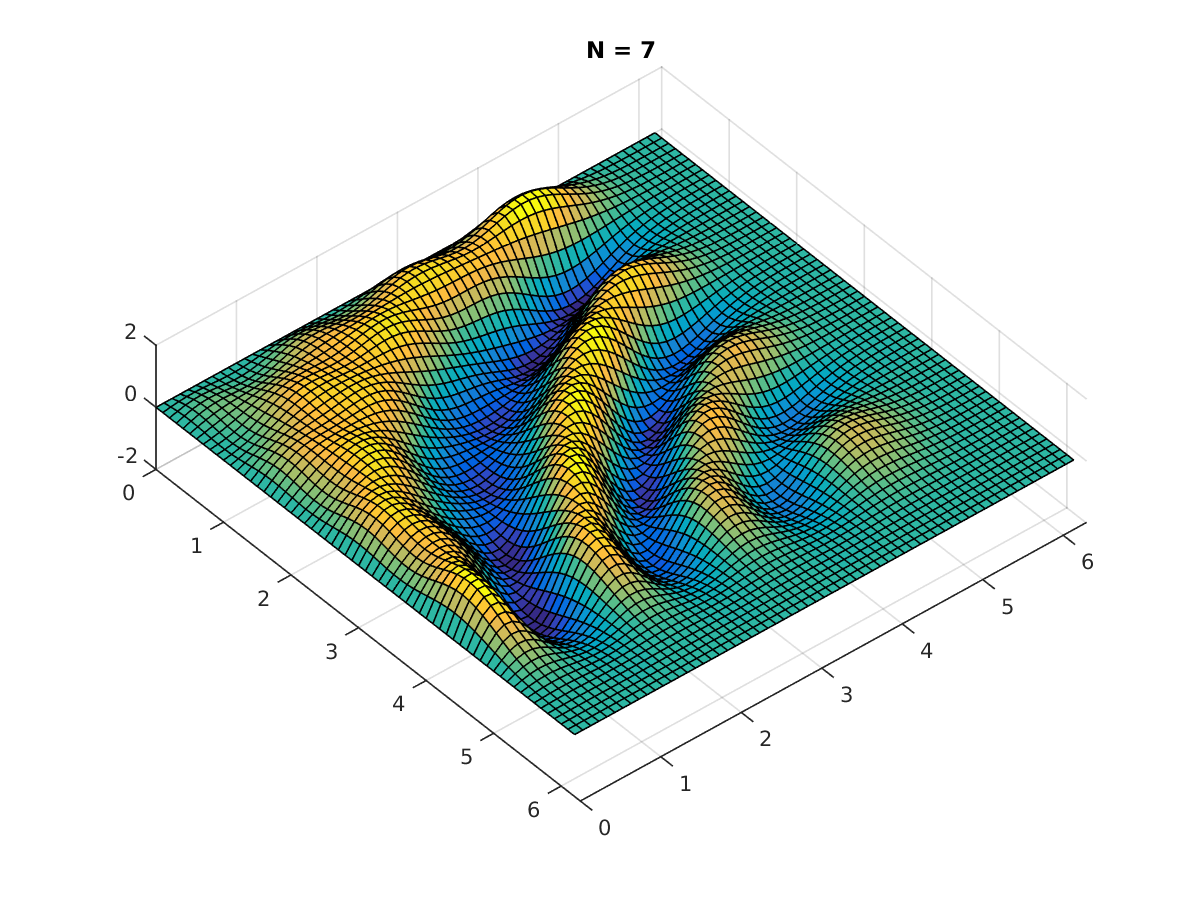
\includegraphics [scale=0.415]{as/a7.png}
\end{figure}
\end{frame}

\begin{frame}
\frametitle{Linear Algebra}
\framesubtitle{SVD: successive matrix reconstruction {\tiny cont.}} 
\small{
\begin{center}
\begin{align*}
Z &= sin(xy) \\
  &= \lambda_k{\bf u}_k {\bf v}_k^T
\end{align*}
\end{center}}
\begin{figure}[!htb]
\centering
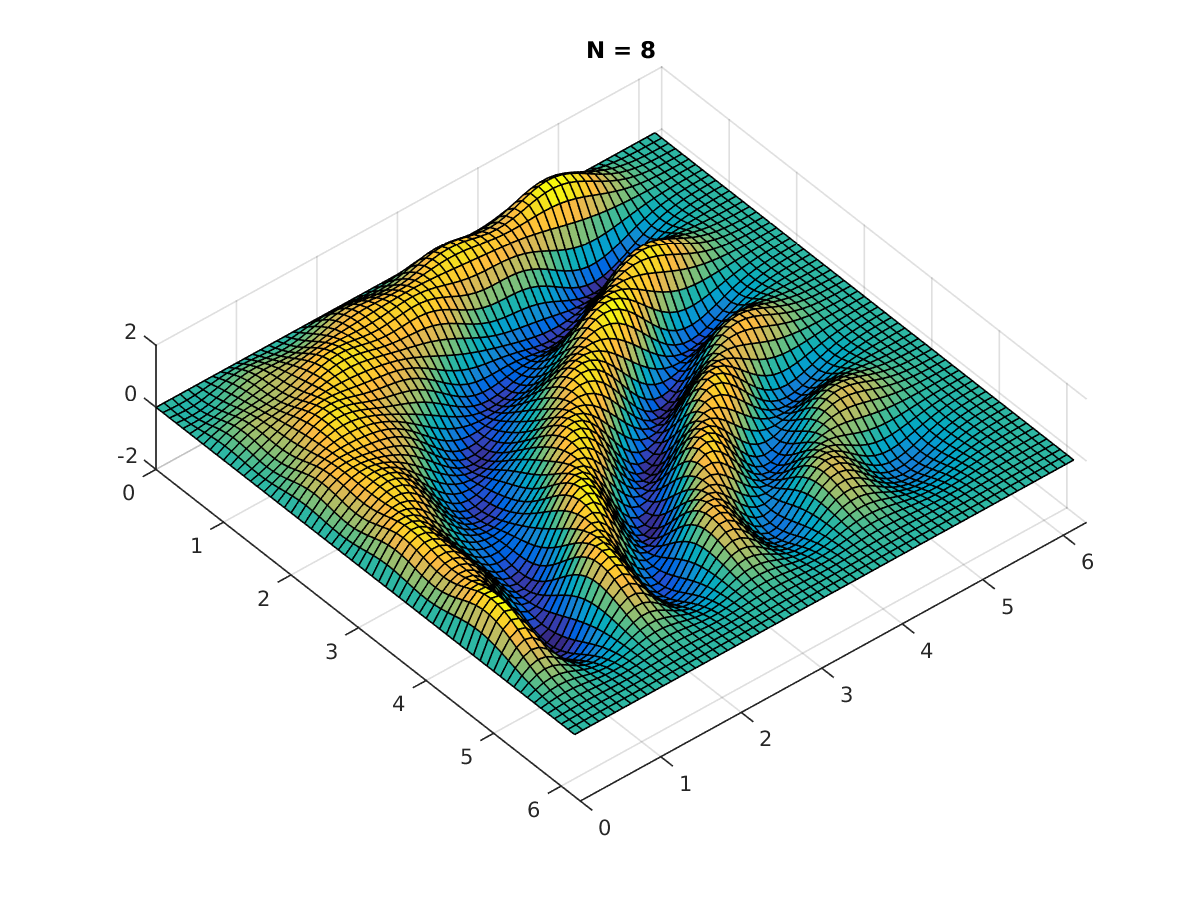
\includegraphics [scale=0.415]{as/a8.png}
\end{figure}
\end{frame}

\begin{frame}
\frametitle{Linear Algebra}
\framesubtitle{SVD: successive matrix reconstruction {\tiny cont.}} 
\small{
\begin{center}
\begin{align*}
Z &= sin(xy) \\
  &= \lambda_k{\bf u}_k {\bf v}_k^T
\end{align*}
\end{center}}
\begin{figure}[!htb]
\centering
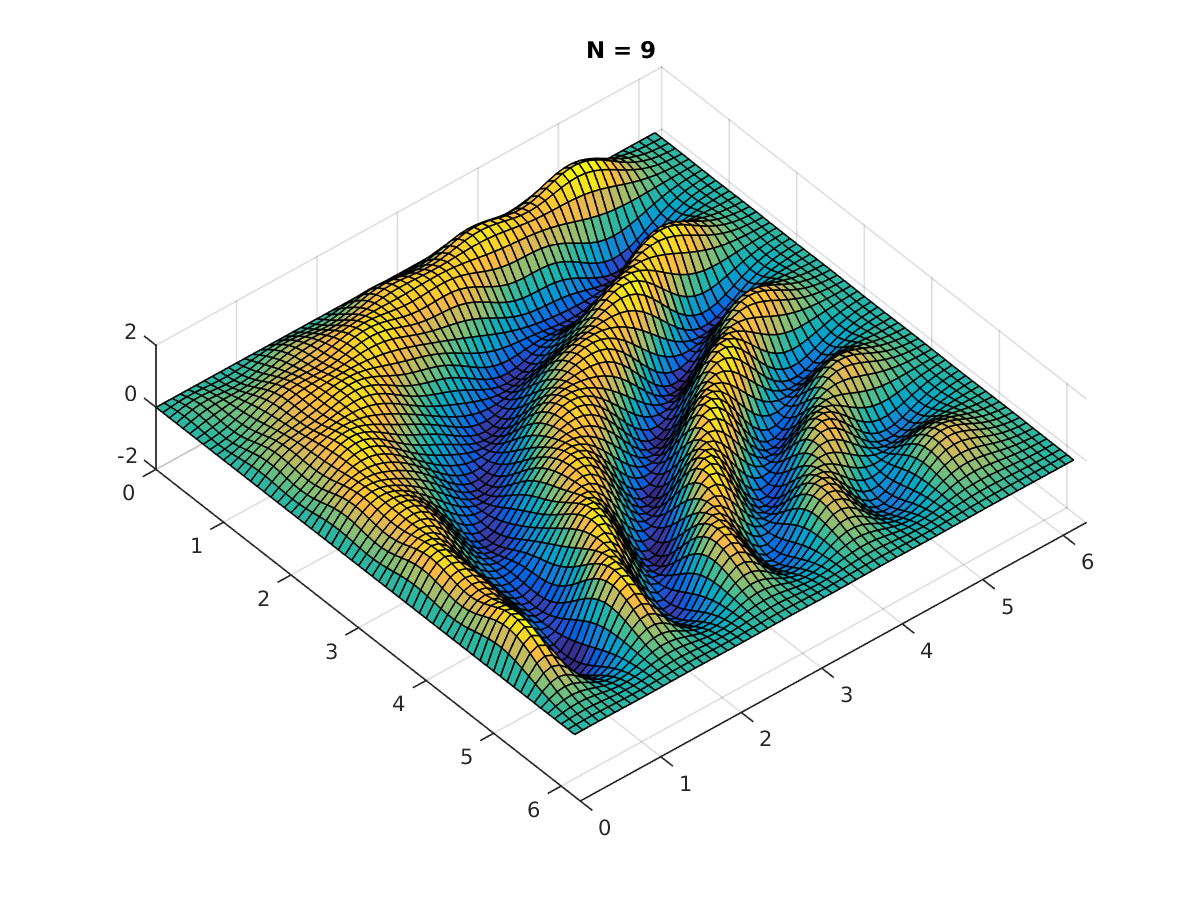
\includegraphics [scale=0.415]{as/a9.png}
\end{figure}
\end{frame}

\begin{frame}
\frametitle{Linear Algebra}
\framesubtitle{SVD: successive matrix reconstruction {\tiny cont.}} 
\small{
\begin{center}
\begin{align*}
Z &= sin(xy) \\
  &= \lambda_k{\bf u}_k {\bf v}_k^T
\end{align*}
\end{center}}
\begin{figure}[!htb]
\centering
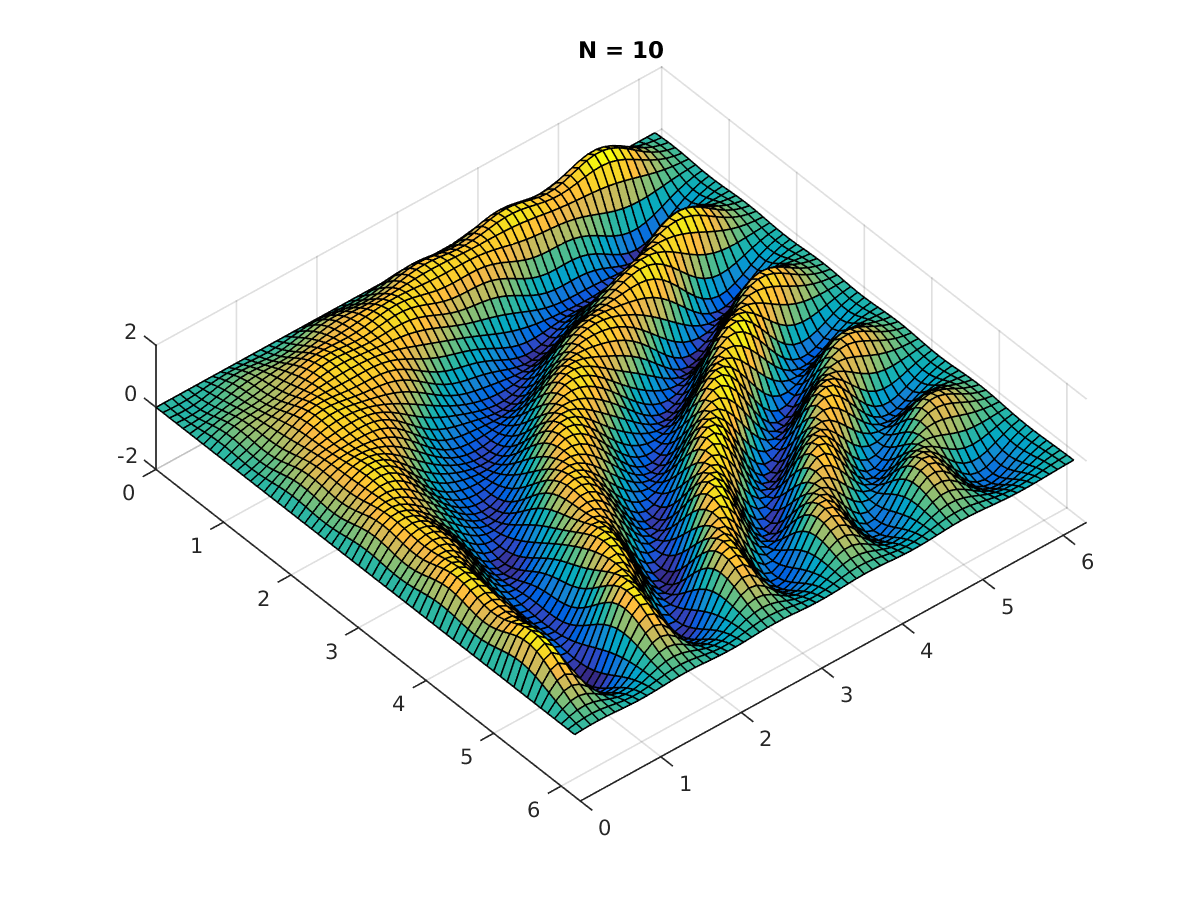
\includegraphics [scale=0.415]{as/a10.png}
\end{figure}
\end{frame}

\begin{frame}
\frametitle{Linear Algebra}
\framesubtitle{SVD: successive matrix reconstruction {\tiny cont.}} 
\small{
\begin{center}
\begin{align*}
Z &= sin(xy) \\
  &= \lambda_k{\bf u}_k {\bf v}_k^T
\end{align*}
\end{center}}
\begin{figure}[!htb]
\centering
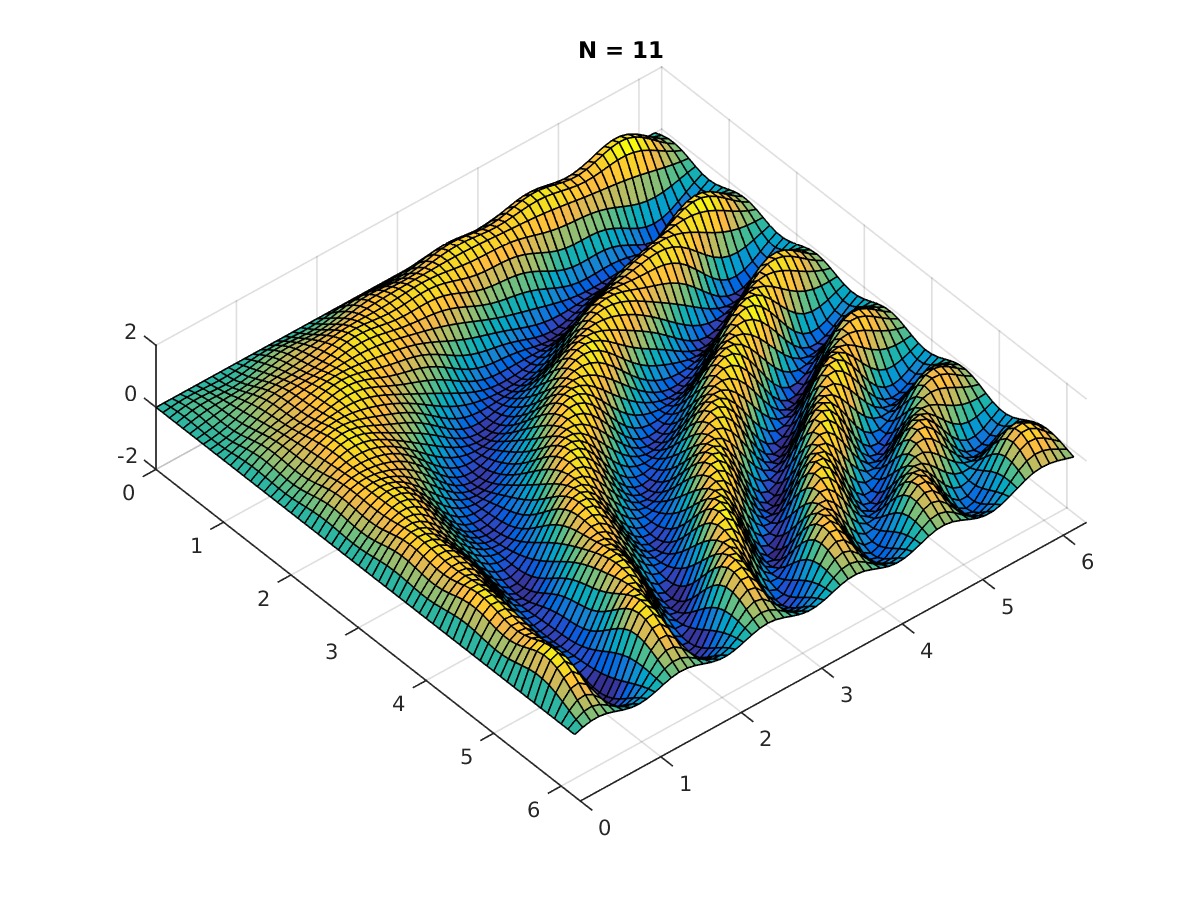
\includegraphics [scale=0.415]{as/a11.png}
\end{figure}
\end{frame}


\begin{frame}
\frametitle{Linear Algebra}
\framesubtitle{SVD: successive matrix reconstruction {\tiny cont.}} 
\small{
\begin{center}
\begin{align*}
Z &= sin(xy) \\
  &= \lambda_k{\bf u}_k {\bf v}_k^T
\end{align*}
\end{center}}
\begin{figure}[!htb]
\centering
\includegraphics [scale=0.415]{as/a12.png}
\end{figure}
\end{frame}

\begin{frame}
\frametitle{Linear Algebra}
\framesubtitle{SVD: successive matrix reconstruction {\tiny cont.}} 
\small{
\begin{center}
\begin{align*}
Z &= sin(xy) \\
  &= \lambda_k{\bf u}_k {\bf v}_k^T
\end{align*}
\end{center}}
\begin{figure}[!htb]
\centering
\includegraphics [scale=0.415]{as/a13.png}
\end{figure}
\end{frame}

\begin{frame}
\frametitle{Linear Algebra}
\framesubtitle{SVD: successive matrix reconstruction {\tiny cont.}} 
\small{
\begin{center}
\begin{align*}
Z &= sin(xy) \\
  &= \lambda_k{\bf u}_k {\bf v}_k^T
\end{align*}
\end{center}}
\begin{figure}[!htb]
\centering
\includegraphics [scale=0.415]{as/a14.png}
\end{figure}
\end{frame}

\subsection{Image reconstruction}

\begin{frame}
\frametitle{Linear Algebra}
\framesubtitle{SVD: successive image reconstruction } 
\scriptsize{
\begin{itemize}
\item Original image size: 339$\times$262
\item Max N: 339
\end{itemize}}
\begin{figure}[!htb]
\centering
\includegraphics [scale=0.48]{figs/b262.png}
\end{figure}
\end{frame}

\begin{frame}
\frametitle{Linear Algebra}
\framesubtitle{SVD: successive image reconstruction} 
\small{
\begin{center}
$Image = \lambda_k{\bf u}_k {\bf v}_k^T$
\end{center}}
\begin{figure}[!htb]
\centering
\includegraphics [scale=0.48]{n/b1.png}
\end{figure}
\end{frame}

\begin{frame}
\frametitle{Linear Algebra}
\framesubtitle{SVD: successive image reconstruction} 
\small{
\begin{center}
$Image = \lambda_k{\bf u}_k {\bf v}_k^T$
\end{center}}
\begin{figure}[!htb]
\centering
\includegraphics [scale=0.48]{n/b2.png}
\end{figure}
\end{frame}

\begin{frame}
\frametitle{Linear Algebra}
\framesubtitle{SVD: successive image reconstruction} 
\small{
\begin{center}
$Image = \lambda_k{\bf u}_k {\bf v}_k^T$
\end{center}}
\begin{figure}[!htb]
\centering
\includegraphics [scale=0.48]{n/b3.png}
\end{figure}
\end{frame}

\begin{frame}
\frametitle{Linear Algebra}
\framesubtitle{SVD: successive image reconstruction} 
\small{
\begin{center}
$Image = \lambda_k{\bf u}_k {\bf v}_k^T$
\end{center}}
\begin{figure}[!htb]
\centering
\includegraphics [scale=0.48]{n/b4.png}
\end{figure}
\end{frame}

\begin{frame}
\frametitle{Linear Algebra}
\framesubtitle{SVD: successive image reconstruction} 
\small{
\begin{center}
$Image = \lambda_k{\bf u}_k {\bf v}_k^T$
\end{center}}
\begin{figure}[!htb]
\centering
\includegraphics [scale=0.48]{n/b5.png}
\end{figure}
\end{frame}

\begin{frame}
\frametitle{Linear Algebra}
\framesubtitle{SVD: successive image reconstruction} 
\small{
\begin{center}
$Image = \lambda_k{\bf u}_k {\bf v}_k^T$
\end{center}}
\begin{figure}[!htb]
\centering
\includegraphics [scale=0.48]{n/b6.png}
\end{figure}
\end{frame}

\begin{frame}
\frametitle{Linear Algebra}
\framesubtitle{SVD: successive image reconstruction} 
\small{
\begin{center}
$Image = \lambda_k{\bf u}_k {\bf v}_k^T$
\end{center}}
\begin{figure}[!htb]
\centering
\includegraphics [scale=0.48]{n/b7.png}
\end{figure}
\end{frame}

\begin{frame}
\frametitle{Linear Algebra}
\framesubtitle{SVD: successive image reconstruction} 
\small{
\begin{center}
$Image = \lambda_k{\bf u}_k {\bf v}_k^T$
\end{center}}
\begin{figure}[!htb]
\centering
\includegraphics [scale=0.48]{n/b8.png}
\end{figure}
\end{frame}

\begin{frame}
\frametitle{Linear Algebra}
\framesubtitle{SVD: successive image reconstruction} 
\small{
\begin{center}
$Image = \lambda_k{\bf u}_k {\bf v}_k^T$
\end{center}}
\begin{figure}[!htb]
\centering
\includegraphics [scale=0.48]{n/b9.png}
\end{figure}
\end{frame}

\begin{frame}
\frametitle{Linear Algebra}
\framesubtitle{SVD: successive image reconstruction} 
\small{
\begin{center}
$Image = \lambda_k{\bf u}_k {\bf v}_k^T$
\end{center}}
\begin{figure}[!htb]
\centering
\includegraphics [scale=0.48]{n/b10.png}
\end{figure}
\end{frame}


\begin{frame}
\frametitle{Linear Algebra}
\framesubtitle{SVD: successive image reconstruction} 
\small{
\begin{center}
$Image = \lambda_k{\bf u}_k {\bf v}_k^T$
\end{center}}
\begin{figure}[!htb]
\centering
\includegraphics [scale=0.48]{n/b11.png}
\end{figure}
\end{frame}

\begin{frame}
\frametitle{Linear Algebra}
\framesubtitle{SVD: successive image reconstruction} 
\small{
\begin{center}
$Image = \lambda_k{\bf u}_k {\bf v}_k^T$
\end{center}}
\begin{figure}[!htb]
\centering
\includegraphics [scale=0.48]{n/b12.png}
\end{figure}
\end{frame}

\begin{frame}
\frametitle{Linear Algebra}
\framesubtitle{SVD: successive image reconstruction} 
\small{
\begin{center}
$Image = \lambda_k{\bf u}_k {\bf v}_k^T$
\end{center}}
\begin{figure}[!htb]
\centering
\includegraphics [scale=0.48]{n/b13.png}
\end{figure}
\end{frame}

\begin{frame}
\frametitle{Linear Algebra}
\framesubtitle{SVD: successive image reconstruction} 
\small{
\begin{center}
$Image = \lambda_k{\bf u}_k {\bf v}_k^T$
\end{center}}
\begin{figure}[!htb]
\centering
\includegraphics [scale=0.48]{n/b14.png}
\end{figure}
\end{frame}

\begin{frame}
\frametitle{Linear Algebra}
\framesubtitle{SVD: successive image reconstruction} 
\small{
\begin{center}
$Image = \lambda_k{\bf u}_k {\bf v}_k^T$
\end{center}}
\begin{figure}[!htb]
\centering
\includegraphics [scale=0.48]{n/b15.png}
\end{figure}
\end{frame}

\begin{frame}
\frametitle{Linear Algebra}
\framesubtitle{SVD: successive image reconstruction} 
\small{
\begin{center}
$Image = \lambda_k{\bf u}_k {\bf v}_k^T$
\end{center}}
\begin{figure}[!htb]
\centering
\includegraphics [scale=0.48]{n/b16.png}
\end{figure}
\end{frame}

\begin{frame}
\frametitle{Linear Algebra}
\framesubtitle{SVD: successive image reconstruction} 
\small{
\begin{center}
$Image = \lambda_k{\bf u}_k {\bf v}_k^T$
\end{center}}
\begin{figure}[!htb]
\centering
\includegraphics [scale=0.48]{n/b16.png}
\end{figure}
\end{frame}

\begin{frame}
\frametitle{Linear Algebra}
\framesubtitle{SVD: successive image reconstruction} 
\small{
\begin{center}
$Image = \lambda_k{\bf u}_k {\bf v}_k^T$
\end{center}}
\begin{figure}[!htb]
\centering
\includegraphics [scale=0.48]{n/b17.png}
\end{figure}
\end{frame}

\begin{frame}
\frametitle{Linear Algebra}
\framesubtitle{SVD: successive image reconstruction} 
\small{
\begin{center}
$Image = \lambda_k{\bf u}_k {\bf v}_k^T$
\end{center}}
\begin{figure}[!htb]
\centering
\includegraphics [scale=0.48]{n/b18.png}
\end{figure}
\end{frame}

\begin{frame}
\frametitle{Linear Algebra}
\framesubtitle{SVD: successive image reconstruction} 
\small{
\begin{center}
$Image = \lambda_k{\bf u}_k {\bf v}_k^T$
\end{center}}
\begin{figure}[!htb]
\centering
\includegraphics [scale=0.48]{n/b19.png}
\end{figure}
\end{frame}

\begin{frame}
\frametitle{Linear Algebra}
\framesubtitle{SVD: successive image reconstruction} 
\small{
\begin{center}
$Image = \lambda_k{\bf u}_k {\bf v}_k^T$
\end{center}}
\begin{figure}[!htb]
\centering
\includegraphics [scale=0.48]{n/b20.png}
\end{figure}
\end{frame}

\begin{frame}
\frametitle{Linear Algebra}
\framesubtitle{SVD: successive image reconstruction} 
\small{
\begin{center}
$Image = \lambda_k{\bf u}_k {\bf v}_k^T$
\end{center}}
\begin{figure}[!htb]
\centering
\includegraphics [scale=0.48]{n/b21.png}
\end{figure}
\end{frame}

\begin{frame}
\frametitle{Linear Algebra}
\framesubtitle{SVD: successive image reconstruction} 
\small{
\begin{center}
$Image = \lambda_k{\bf u}_k {\bf v}_k^T$
\end{center}}
\begin{figure}[!htb]
\centering
\includegraphics [scale=0.48]{n/b22.png}
\end{figure}
\end{frame}

\begin{frame}
\frametitle{Linear Algebra}
\framesubtitle{SVD: successive image reconstruction} 
\small{
\begin{center}
$Image = \lambda_k{\bf u}_k {\bf v}_k^T$
\end{center}}
\begin{figure}[!htb]
\centering
\includegraphics [scale=0.48]{n/b23.png}
\end{figure}
\end{frame}


\begin{frame}
\frametitle{Linear Algebra}
\framesubtitle{SVD: successive image reconstruction} 
\small{
\begin{center}
$Image = \lambda_k{\bf u}_k {\bf v}_k^T$
\end{center}}
\begin{figure}[!htb]
\centering
\includegraphics [scale=0.48]{n/b24.png}
\end{figure}
\end{frame}

\begin{frame}
\frametitle{Linear Algebra}
\framesubtitle{SVD: successive image reconstruction} 
\small{
\begin{center}
$Image = \lambda_k{\bf u}_k {\bf v}_k^T$
\end{center}}
\begin{figure}[!htb]
\centering
\includegraphics [scale=0.48]{n/b25.png}
\end{figure}
\end{frame}

\begin{frame}
\frametitle{Linear Algebra}
\framesubtitle{SVD: successive image reconstruction} 
\small{
\begin{center}
$Image = \lambda_k{\bf u}_k {\bf v}_k^T$
\end{center}}
\begin{figure}[!htb]
\centering
\includegraphics [scale=0.48]{n/b26.png}
\end{figure}
\end{frame}

\begin{frame}
\frametitle{Linear Algebra}
\framesubtitle{SVD: successive image reconstruction} 
\small{
\begin{center}
$Image = \lambda_k{\bf u}_k {\bf v}_k^T$
\end{center}}
\begin{figure}[!htb]
\centering
\includegraphics [scale=0.48]{n/b27.png}
\end{figure}
\end{frame}

\begin{frame}
\frametitle{Linear Algebra}
\framesubtitle{SVD: successive image reconstruction} 
\small{
\begin{center}
$Image = \lambda_k{\bf u}_k {\bf v}_k^T$
\end{center}}
\begin{figure}[!htb]
\centering
\includegraphics [scale=0.48]{n/b28.png}
\end{figure}
\end{frame}

\begin{frame}
\frametitle{Linear Algebra}
\framesubtitle{SVD: successive image reconstruction} 
\small{
\begin{center}
$Image = \lambda_k{\bf u}_k {\bf v}_k^T$
\end{center}}
\begin{figure}[!htb]
\centering
\includegraphics [scale=0.48]{n/b29.png}
\end{figure}
\end{frame}

\begin{frame}
\frametitle{Linear Algebra}
\framesubtitle{SVD: successive image reconstruction} 
\small{
\begin{center}
$Image = \lambda_k{\bf u}_k {\bf v}_k^T$
\end{center}}
\begin{figure}[!htb]
\centering
\includegraphics [scale=0.48]{n/b30.png}
\end{figure}
\end{frame}


\begin{frame}
\frametitle{Linear Algebra}
\framesubtitle{SVD: successive image reconstruction} 
\small{
\begin{center}
$Image = \lambda_k{\bf u}_k {\bf v}_k^T$
\end{center}}
\begin{figure}[!htb]
\centering
\includegraphics [scale=0.48]{n/b31.png}
\end{figure}
\end{frame}

\begin{frame}
\frametitle{Linear Algebra}
\framesubtitle{SVD: successive image reconstruction} 
\small{
\begin{center}
$Image = \lambda_k{\bf u}_k {\bf v}_k^T$
\end{center}}
\begin{figure}[!htb]
\centering
\includegraphics [scale=0.48]{n/b32.png}
\end{figure}
\end{frame}

\begin{frame}
\frametitle{Linear Algebra}
\framesubtitle{SVD: successive image reconstruction} 
\small{
\begin{center}
$Image = \lambda_k{\bf u}_k {\bf v}_k^T$
\end{center}}
\begin{figure}[!htb]
\centering
\includegraphics [scale=0.48]{n/b33.png}
\end{figure}
\end{frame}


\begin{frame}
\frametitle{Linear Algebra}
\framesubtitle{SVD: successive image reconstruction} 
\small{
\begin{center}
$Image = \lambda_k{\bf u}_k {\bf v}_k^T$
\end{center}}
\begin{figure}[!htb]
\centering
\includegraphics [scale=0.48]{n/b34.png}
\end{figure}
\end{frame}

\begin{frame}
\frametitle{Linear Algebra}
\framesubtitle{SVD: successive image reconstruction} 
\small{
\begin{center}
$Image = \lambda_k{\bf u}_k {\bf v}_k^T$
\end{center}}
\begin{figure}[!htb]
\centering
\includegraphics [scale=0.48]{n/b35.png}
\end{figure}
\end{frame}

\begin{frame}
\frametitle{Linear Algebra}
\framesubtitle{SVD: successive image reconstruction} 
\small{
\begin{center}
$Image = \lambda_k{\bf u}_k {\bf v}_k^T$
\end{center}}
\begin{figure}[!htb]
\centering
\includegraphics [scale=0.48]{n/b36.png}
\end{figure}
\end{frame}

\begin{frame}
\frametitle{Linear Algebra}
\framesubtitle{SVD: successive image reconstruction} 
\small{
\begin{center}
$Image = \lambda_k{\bf u}_k {\bf v}_k^T$
\end{center}}
\begin{figure}[!htb]
\centering
\includegraphics [scale=0.48]{n/b37.png}
\end{figure}
\end{frame}

\begin{frame}
\frametitle{Linear Algebra}
\framesubtitle{SVD: successive image reconstruction} 
\small{
\begin{center}
$Image = \lambda_k{\bf u}_k {\bf v}_k^T$
\end{center}}
\begin{figure}[!htb]
\centering
\includegraphics [scale=0.48]{n/b38.png}
\end{figure}
\end{frame}

\begin{frame}
\frametitle{Linear Algebra}
\framesubtitle{SVD: successive image reconstruction} 
\small{
\begin{center}
$Image = \lambda_k{\bf u}_k {\bf v}_k^T$
\end{center}}
\begin{figure}[!htb]
\centering
\includegraphics [scale=0.48]{n/b39.png}
\end{figure}
\end{frame}

\begin{frame}
\frametitle{Linear Algebra}
\framesubtitle{SVD: successive image reconstruction} 
\small{
\begin{center}
$Image = \lambda_k{\bf u}_k {\bf v}_k^T$
\end{center}}
\begin{figure}[!htb]
\centering
\includegraphics [scale=0.48]{n/b40.png}
\end{figure}
\end{frame}

\begin{frame}
\frametitle{Linear Algebra}
\framesubtitle{SVD: successive image reconstruction} 
\small{
\begin{center}
$Image = \lambda_k{\bf u}_k {\bf v}_k^T$
\end{center}}
\begin{figure}[!htb]
\centering
\includegraphics [scale=0.48]{n/b41.png}
\end{figure}
\end{frame}

\begin{frame}
\frametitle{Linear Algebra}
\framesubtitle{SVD: successive image reconstruction} 
\small{
\begin{center}
$Image = \lambda_k{\bf u}_k {\bf v}_k^T$
\end{center}}
\begin{figure}[!htb]
\centering
\includegraphics [scale=0.48]{n/b42.png}
\end{figure}
\end{frame}

\begin{frame}
\frametitle{Linear Algebra}
\framesubtitle{SVD: successive image reconstruction} 
\small{
\begin{center}
$Image = \lambda_k{\bf u}_k {\bf v}_k^T$
\end{center}}
\begin{figure}[!htb]
\centering
\includegraphics [scale=0.48]{n/b43.png}
\end{figure}
\end{frame}

\begin{frame}
\frametitle{Linear Algebra}
\framesubtitle{SVD: successive image reconstruction} 
\small{
\begin{center}
$Image = \lambda_k{\bf u}_k {\bf v}_k^T$
\end{center}}
\begin{figure}[!htb]
\centering
\includegraphics [scale=0.48]{n/b44.png}
\end{figure}
\end{frame}

\begin{frame}
\frametitle{Linear Algebra}
\framesubtitle{SVD: successive image reconstruction} 
\small{
\begin{center}
$Image = \lambda_k{\bf u}_k {\bf v}_k^T$
\end{center}}
\begin{figure}[!htb]
\centering
\includegraphics [scale=0.48]{n/b45.png}
\end{figure}
\end{frame}

\begin{frame}
\frametitle{Linear Algebra}
\framesubtitle{SVD: successive image reconstruction} 
\small{
\begin{center}
$Image = \lambda_k{\bf u}_k {\bf v}_k^T$
\end{center}}
\begin{figure}[!htb]
\centering
\includegraphics [scale=0.48]{n/b46.png}
\end{figure}
\end{frame}

\begin{frame}
\frametitle{Linear Algebra}
\framesubtitle{SVD: successive image reconstruction} 
\small{
\begin{center}
$Image = \lambda_k{\bf u}_k {\bf v}_k^T$
\end{center}}
\begin{figure}[!htb]
\centering
\includegraphics [scale=0.48]{n/b47.png}
\end{figure}
\end{frame}

\begin{frame}
\frametitle{Linear Algebra}
\framesubtitle{SVD: successive image reconstruction} 
\small{
\begin{center}
$Image = \lambda_k{\bf u}_k {\bf v}_k^T$
\end{center}}
\begin{figure}[!htb]
\centering
\includegraphics [scale=0.48]{n/b48.png}
\end{figure}
\end{frame}

\begin{frame}
\frametitle{Linear Algebra}
\framesubtitle{SVD: successive image reconstruction} 
\small{
\begin{center}
$Image = \lambda_k{\bf u}_k {\bf v}_k^T$
\end{center}}
\begin{figure}[!htb]
\centering
\includegraphics [scale=0.48]{n/b49.png}
\end{figure}
\end{frame}

\begin{frame}
\frametitle{Linear Algebra}
\framesubtitle{SVD: successive image reconstruction} 
\small{
\begin{center}
$Image = \lambda_k{\bf u}_k {\bf v}_k^T$
\end{center}}
\begin{figure}[!htb]
\centering
\includegraphics [scale=0.48]{n/b50.png}
\end{figure}
\end{frame}

\begin{frame}
\frametitle{Linear Algebra}
\framesubtitle{SVD: successive image reconstruction} 
\small{
\begin{center}
$Image = \lambda_k{\bf u}_k {\bf v}_k^T$
\end{center}}
\begin{figure}[!htb]
\centering
\includegraphics [scale=0.48]{n/b51.png}
\end{figure}
\end{frame}

\begin{frame}
\frametitle{Linear Algebra}
\framesubtitle{SVD: successive image reconstruction} 
\small{
\begin{center}
$Image = \lambda_k{\bf u}_k {\bf v}_k^T$
\end{center}}
\begin{figure}[!htb]
\centering
\includegraphics [scale=0.48]{n/b52.png}
\end{figure}
\end{frame}

\begin{frame}
\frametitle{Linear Algebra}
\framesubtitle{SVD: successive image reconstruction} 
\small{
\begin{center}
$Image = \lambda_k{\bf u}_k {\bf v}_k^T$
\end{center}}
\begin{figure}[!htb]
\centering
\includegraphics [scale=0.48]{n/b53.png}
\end{figure}
\end{frame}

\begin{frame}
\frametitle{Linear Algebra}
\framesubtitle{SVD: successive image reconstruction} 
\small{
\begin{center}
$Image = \lambda_k{\bf u}_k {\bf v}_k^T$
\end{center}}
\begin{figure}[!htb]
\centering
\includegraphics [scale=0.48]{n/b54.png}
\end{figure}
\end{frame}

\begin{frame}
\frametitle{Linear Algebra}
\framesubtitle{SVD: successive image reconstruction} 
\small{
\begin{center}
$Image = \lambda_k{\bf u}_k {\bf v}_k^T$
\end{center}}
\begin{figure}[!htb]
\centering
\includegraphics [scale=0.48]{n/b55.png}
\end{figure}
\end{frame}

\begin{frame}
\frametitle{Linear Algebra}
\framesubtitle{SVD: successive image reconstruction} 
\small{
\begin{center}
$Image = \lambda_k{\bf u}_k {\bf v}_k^T$
\end{center}}
\begin{figure}[!htb]
\centering
\includegraphics [scale=0.48]{n/b56.png}
\end{figure}
\end{frame}

\begin{frame}
\frametitle{Linear Algebra}
\framesubtitle{SVD: successive image reconstruction} 
\small{
\begin{center}
$Image = \lambda_k{\bf u}_k {\bf v}_k^T$
\end{center}}
\begin{figure}[!htb]
\centering
\includegraphics [scale=0.48]{n/b57.png}
\end{figure}
\end{frame}

\begin{frame}
\frametitle{Linear Algebra}
\framesubtitle{SVD: successive image reconstruction} 
\small{
\begin{center}
$Image = \lambda_k{\bf u}_k {\bf v}_k^T$
\end{center}}
\begin{figure}[!htb]
\centering
\includegraphics [scale=0.48]{n/b58.png}
\end{figure}
\end{frame}

\begin{frame}
\frametitle{Linear Algebra}
\framesubtitle{SVD: successive image reconstruction} 
\small{
\begin{center}
$Image = \lambda_k{\bf u}_k {\bf v}_k^T$
\end{center}}
\begin{figure}[!htb]
\centering
\includegraphics [scale=0.48]{n/b59.png}
\end{figure}
\end{frame}

\begin{frame}
\frametitle{Linear Algebra}
\framesubtitle{SVD: successive image reconstruction} 
\small{
\begin{center}
$Image = \lambda_k{\bf u}_k {\bf v}_k^T$
\end{center}}
\begin{figure}[!htb]
\centering
\includegraphics [scale=0.48]{n/b60.png}
\end{figure}
\end{frame}

\begin{frame}
\frametitle{Linear Algebra}
\framesubtitle{SVD: successive image reconstruction} 
\small{
\begin{center}
$Image = \lambda_k{\bf u}_k {\bf v}_k^T$
\end{center}}
\begin{figure}[!htb]
\centering
\includegraphics [scale=0.48]{n/b61.png}
\end{figure}
\end{frame}

\begin{frame}
\frametitle{Linear Algebra}
\framesubtitle{SVD: successive image reconstruction} 
\small{
\begin{center}
$Image = \lambda_k{\bf u}_k {\bf v}_k^T$
\end{center}}
\begin{figure}[!htb]
\centering
\includegraphics [scale=0.48]{n/b62.png}
\end{figure}
\end{frame}

\begin{frame}
\frametitle{Linear Algebra}
\framesubtitle{SVD: successive image reconstruction} 
\small{
\begin{center}
$Image = \lambda_k{\bf u}_k {\bf v}_k^T$
\end{center}}
\begin{figure}[!htb]
\centering
\includegraphics [scale=0.48]{n/b63.png}
\end{figure}
\end{frame}

\begin{frame}
\frametitle{Linear Algebra}
\framesubtitle{SVD: successive image reconstruction} 
\small{
\begin{center}
$Image = \lambda_k{\bf u}_k {\bf v}_k^T$
\end{center}}
\begin{figure}[!htb]
\centering
\includegraphics [scale=0.48]{n/b64.png}
\end{figure}
\end{frame}

\begin{frame}
\frametitle{Linear Algebra}
\framesubtitle{SVD: successive image reconstruction} 
\small{
\begin{center}
$Image = \lambda_k{\bf u}_k {\bf v}_k^T$
\end{center}}
\begin{figure}[!htb]
\centering
\includegraphics [scale=0.48]{n/b65.png}
\end{figure}
\end{frame}

\begin{frame}
\frametitle{Linear Algebra}
\framesubtitle{SVD: successive image reconstruction} 
\small{
\begin{center}
$Image = \lambda_k{\bf u}_k {\bf v}_k^T$
\end{center}}
\begin{figure}[!htb]
\centering
\includegraphics [scale=0.48]{n/b66.png}
\end{figure}
\end{frame}

\begin{frame}
\frametitle{Linear Algebra}
\framesubtitle{SVD: successive image reconstruction} 
\small{
\begin{center}
$Image = \lambda_k{\bf u}_k {\bf v}_k^T$
\end{center}}
\begin{figure}[!htb]
\centering
\includegraphics [scale=0.48]{n/b67.png}
\end{figure}
\end{frame}

\begin{frame}
\frametitle{Linear Algebra}
\framesubtitle{SVD: successive image reconstruction} 
\small{
\begin{center}
$Image = \lambda_k{\bf u}_k {\bf v}_k^T$
\end{center}}
\begin{figure}[!htb]
\centering
\includegraphics [scale=0.48]{n/b68.png}
\end{figure}
\end{frame}

\begin{frame}
\frametitle{Linear Algebra}
\framesubtitle{SVD: successive image reconstruction} 
\small{
\begin{center}
$Image = \lambda_k{\bf u}_k {\bf v}_k^T$
\end{center}}
\begin{figure}[!htb]
\centering
\includegraphics [scale=0.48]{n/b69.png}
\end{figure}
\end{frame}

\begin{frame}
\frametitle{Linear Algebra}
\framesubtitle{SVD: successive image reconstruction} 
\small{
\begin{center}
$Image = \lambda_k{\bf u}_k {\bf v}_k^T$
\end{center}}
\begin{figure}[!htb]
\centering
\includegraphics [scale=0.48]{n/b70.png}
\end{figure}
\end{frame}

\begin{frame}
\frametitle{Linear Algebra}
\framesubtitle{SVD: successive image reconstruction} 
\small{
\begin{center}
$Image = \lambda_k{\bf u}_k {\bf v}_k^T$
\end{center}}
\begin{figure}[!htb]
\centering
\includegraphics [scale=0.48]{n/b71.png}
\end{figure}
\end{frame}

\begin{frame}
\frametitle{Linear Algebra}
\framesubtitle{SVD: successive image reconstruction} 
\small{
\begin{center}
$Image = \lambda_k{\bf u}_k {\bf v}_k^T$
\end{center}}
\begin{figure}[!htb]
\centering
\includegraphics [scale=0.48]{n/b72.png}
\end{figure}
\end{frame}

\begin{frame}
\frametitle{Linear Algebra}
\framesubtitle{SVD: successive image reconstruction} 
\small{
\begin{center}
$Image = \lambda_k{\bf u}_k {\bf v}_k^T$
\end{center}}
\begin{figure}[!htb]
\centering
\includegraphics [scale=0.48]{n/b73.png}
\end{figure}
\end{frame}

\begin{frame}
\frametitle{Linear Algebra}
\framesubtitle{SVD: successive image reconstruction} 
\small{
\begin{center}
$Image = \lambda_k{\bf u}_k {\bf v}_k^T$
\end{center}}
\begin{figure}[!htb]
\centering
\includegraphics [scale=0.48]{n/b74.png}
\end{figure}
\end{frame}

\begin{frame}
\frametitle{Linear Algebra}
\framesubtitle{SVD: successive image reconstruction} 
\small{
\begin{center}
$Image = \lambda_k{\bf u}_k {\bf v}_k^T$
\end{center}}
\begin{figure}[!htb]
\centering
\includegraphics [scale=0.48]{n/b75.png}
\end{figure}
\end{frame}

\begin{frame}
\frametitle{Linear Algebra}
\framesubtitle{SVD: successive image reconstruction} 
\small{
\begin{center}
$Image = \lambda_k{\bf u}_k {\bf v}_k^T$
\end{center}}
\begin{figure}[!htb]
\centering
\includegraphics [scale=0.48]{n/b76.png}
\end{figure}
\end{frame}

\begin{frame}
\frametitle{Linear Algebra}
\framesubtitle{SVD: successive image reconstruction} 
\small{
\begin{center}
$Image = \lambda_k{\bf u}_k {\bf v}_k^T$
\end{center}}
\begin{figure}[!htb]
\centering
\includegraphics [scale=0.48]{n/b77.png}
\end{figure}
\end{frame}

\begin{frame}
\frametitle{Linear Algebra}
\framesubtitle{SVD: successive image reconstruction} 
\small{
\begin{center}
$Image = \lambda_k{\bf u}_k {\bf v}_k^T$
\end{center}}
\begin{figure}[!htb]
\centering
\includegraphics [scale=0.48]{n/b78.png}
\end{figure}
\end{frame}

\begin{frame}
\frametitle{Linear Algebra}
\framesubtitle{SVD: successive image reconstruction} 
\small{
\begin{center}
$Image = \lambda_k{\bf u}_k {\bf v}_k^T$
\end{center}}
\begin{figure}[!htb]
\centering
\includegraphics [scale=0.48]{n/b79.png}
\end{figure}
\end{frame}





\section{Modeling}

\subsection{Electrical}
\begin{frame}
\frametitle{Modeling\\ {\large RLC Circuit}} 
\begin{figure}[!t]
\centering
\includegraphics[scale = 0.35]{figs/Selection_020.png}
\end{figure}
\begin{align}
L \frac{di(t)}{dt}+Ri(t)+\frac{1}{C}q(t)=v(t) \\
 i(t)=\frac{dq(t)}{dt}
\end{align} 
\begin{eqnarray*}
\Rightarrow L\frac{d^2q(t)}{dt^2}+R\frac{dq(t)}{dt}+\frac{1}{C}q(t)=v(t) \\
\Rightarrow L\ddot{q}(t)+R\dot{q}(t)+\frac{1}{C}q(t)=\textcolor{mygreen}{v(t)}
\end{eqnarray*}
\end{frame}

\begin{frame}[shrink]
\frametitle{Modeling {\large Series RLC Circuit}} 
\begin{center}
 \begin{tcolorbox}[title=State Space Representation,width=10 cm]
{
Let,
\begin{center}
\begin{align*}
\textcolor{red}{x_1} &= q(t) \\
\textcolor{blue}{x_2}=\dot{\textcolor{red}{x_1}} &=\dot{q}(t) \\
\dot{\textcolor{blue}{x_2}} &=\ddot{q}(t) 
\end{align*} \end{center}
 Substituting, 
\begin{align*}
L\ddot{q}(t) + R\dot{q}(t) + \frac{1}{C}q(t) &= \textcolor{mygreen}{v(t)} \\
L\dot{\textcolor{blue}{x_2}} + R\textcolor{blue}{x_2} + \frac{1}{C}\textcolor{red}{x_1} &=  \textcolor{mygreen}{v(t)}
\end{align*}
Now Write,
\begin{align*}
\dot{\textcolor{red}{x_1}}&=\textcolor{blue}{x_2} \\
\dot{\textcolor{blue}{x_2}}&=-\frac{1}{LC}\textcolor{red}{x_1}-\frac{R}{L}\textcolor{blue}{x_2}+\frac{1}{L} \textcolor{mygreen}{v(t)} \\
\begin{bmatrix}
\dot{\textcolor{red}{x_1}} \\
\dot{\textcolor{blue}{x_2}}
\end{bmatrix}
&=\begin{bmatrix}
    0     & 1 \\
   -\frac{1}{LC}     &-\frac{R}{L} \\
\end{bmatrix}
\begin{bmatrix}
\textcolor{red}{x_1} \\
\textcolor{blue}{x_2}
\end{bmatrix}+
\begin{bmatrix}
0 \\ \frac{1}{L}
\end{bmatrix}\textcolor{mygreen}{v(t)}
\end{align*}
}
\end{tcolorbox}
\end{center}
\end{frame}







\begin{frame}
\frametitle{Modeling\\ {\large C parallel with RL circuit}} 
\begin{figure}[!t]
\centering
\includegraphics[scale = 0.25]{figs/Selection_021.png}
\end{figure}
\begin{eqnarray*}
i_C=-\textcolor{blue}{i_L}+u(t) \\
\Rightarrow C\frac{d\textcolor{red}{v_C}}{dt}=-\textcolor{blue}{i_L}+u(t) \\
\Rightarrow \frac{d\textcolor{red}{v_C}}{dt}=-\frac{1}{C}\textcolor{blue}{i_L}+\frac{1}{C}u(t)
\\  \newline \newline
V_C=V_L+\textcolor{blue}{i_L}R 
\\ = L\frac{d\textcolor{blue}{i_L}}{dt}+i_LR
\end{eqnarray*}
solve for $\frac{d\textcolor{blue}{i_L}}{dt}$
\end{frame}

\begin{frame}
\frametitle{Modeling\\ {\large C parallel with RL circuit}} 
Starting off with differential equations, we go to state space
\begin{eqnarray*}
\frac{d\textcolor{red}{v_C}}{dt}&=-\frac{1}{C}\textcolor{blue}{i_L}&+\frac{1}{C}\textcolor{mygreen}{u(t)} \\
\frac{d\textcolor{blue}{i_L}}{dt}&=\frac{1}{L}\textcolor{red}{v_C}&-\frac{1}{L}\textcolor{blue}{i_L}R \\ 
\begin{bmatrix}
\dot{\textcolor{red}{V_C}} \\ 
\dot{\textcolor{blue}{i_L}}
\end{bmatrix} &= \begin{bmatrix} 
0 & -\frac{1}{C} \\ 
\frac{1}{L} & -\frac{R}{L}
\end{bmatrix}\begin{bmatrix}
\textcolor{red}{V_C} \\
\textcolor{blue}{i_L}
\end{bmatrix} + \begin{bmatrix}
\frac{1}{C} \\ 0
\end{bmatrix}\textcolor{mygreen}{u(t)}
\end{eqnarray*}
\end{frame}





\subsection{Mechanical}

\begin{frame}
\frametitle{Modeling\\ {\large Constant acceleration model}} 
\tiny{
$$\ddot{s}(t)=a$$
\noindent\makebox[\linewidth]{\rule{10 cm}{0.1pt}}
\begin{align*}
\int_{t_0}^t \ddot{s}(\tau) \ d\tau=\int_{t_0}^t a \ d\tau \\
\textcolor{blue}{\dot{s}}(\tau)|^t_{t_0} = a \  \tau|^t_{t_0} \\
\textcolor{blue}{\dot{s}}(t) - \textcolor{blue}{\dot{s}}(t_0) = at-a\textcolor{red}{t_0}
\end{align*}
\noindent\makebox[\linewidth]{\rule{10 cm}{0.1pt}}
\begin{align*}
\int_{t_0}^t \textcolor{blue}{\dot{s}}(\tau)d\tau - \int_{t_0}^t \textcolor{blue}{\dot{s}}(t_0) d \tau = \int_{t_0}^t a\tau d\tau - \int_{t_0}^t a\textcolor{red}{t_0}d\tau \\
\textcolor{red}{s}(\tau)|^t_{t_0}-\textcolor{blue}{\dot{s}}(t_0)\tau|^t_{t_0}  = \frac{1}{2}a \  \tau^2|^t_{t_0}-at_0\tau|^t_{t_0} \\
\textcolor{red}{s}(t)-\textcolor{red}{s}(t_0)-\textcolor{blue}{\dot s}(t_0)t+\textcolor{blue}{\dot s}(t_0)\textcolor{red}{t_0}=\frac{1}{2}\textcolor{mygreen}{a}t^2-\frac{1}{2}\textcolor{mygreen}{a}\textcolor{red}{t_0}^2-\textcolor{mygreen}{a}\textcolor{red}{t_0}t+\textcolor{mygreen}{a}\textcolor{red}{t_0}^2
\end{align*}
\noindent\makebox[\linewidth]{\rule{10 cm}{0.1pt}}
let initial time $t_0 = 0$, initial distance $\textcolor{red}{s}(t_ 0) = 0$, and some initial velocity
$\textcolor{blue}{\dot s}(t_0) = \textcolor{blue}{v_i}$, to get the familiar equation,
$$\textcolor{red}{s}(t)=\textcolor{blue}{v_i}t+\frac{1}{2}at^2$$
If we take the derivative with respect to t, we get $\textcolor{blue}{v_f}= \textcolor{blue}{v_i} + at$
}
\end{frame}

\begin{frame}
\frametitle{Modeling\\ {\large Constant acceleration model}} 
\begin{itemize}
\item The equations \textcolor{orange}{s} = $\textcolor{blue}{v_i}t$ + $\frac{1}{2}\textcolor{mygreen}{a}t^2$ and $v_f = \textcolor{blue}{v_i} + \textcolor{mygreen}{a}t$ can be written in state space as,
\begin{align*}
\begin{bmatrix}
s \\ v_f
\end{bmatrix} = \begin{bmatrix}
0 & t \\ 0 & 1
\end{bmatrix} \begin{bmatrix}
s_i \\ v_i
\end{bmatrix}+\begin{bmatrix}
\frac{1}{2}t^2 \\ t
\end{bmatrix}
\frac{f}{m}
\end{align*}
and writing in terms of states x and input u, we get, 
\begin{align*}
{\bf x_t} = \begin{bmatrix}
x_t \\ \dot{x}_t
\end{bmatrix}= \begin{bmatrix}
0 & t \\ 0 & 1
\end{bmatrix}
\begin{bmatrix}
x_{t-1} \\ \dot{x}_{t-1}
\end{bmatrix} + \begin{bmatrix}
\frac{\frac{1}{2}t^2}{m} \\ \frac{t}{m}
\end{bmatrix}u
\end{align*}
\item Note that we have used f = m\textcolor{mygreen}{a}, and the input u is the force f
\end{itemize}
\end{frame}











\begin{frame}
\frametitle{Modeling\\ {\large DC Motor {\tiny cont..}}} 
\tiny{

\begin{columns}
    \begin{column}{0.4\textwidth}
\put(-5,210){$\textcolor{red}{v_b}=K_b \omega$} \put(-5,200){$ = K_b \dot{\theta} $ }
\put(25,200){
%\begin{tcolorbox}[colback=mygreen!5,colframe=mygreen!40!black,title=Time Domain]
\colorbox{pink}{\parbox{3.65 cm}{
\centering
Differential equations 
\begin{flushleft}
 \fbox{\begin{minipage}[t]{15em}
\begin{align*}
%\parbox{\textwidth}
\colorbox{cyan}{\hbox to 0.3 mm{L\hfill}} \frac{di}{dt}&+\colorbox{cyan}{\hbox to 0.3 mm{R\hfill}}i=\textcolor{red}{v}-\textcolor{red}{v_b} & \text{1} \\
\colorbox{yellow}{\hbox to 0.3 mm{J\hfill}}\ddot{\theta}&+\colorbox{yellow}{\hbox to 0.3 mm{b\hfill}}\dot{\theta}=\colorbox{  white}{\hbox to 2.2 mm{\textit{${K_m}$}\hfill}}\hspace{1 pt} i  & \text{2}
\end{align*}
\end{minipage}}
\end{flushleft}
%\colorbox{cyan}{\makebox[12em]{\strut\textcolor{black}{R:electrical resistance \ 1 ohm }}}
\colorbox{cyan}{\parbox{2.75 cm}{\color{black}R: electrical resistance \ 1 ohm \\ L: electrical inductance \ 0.5H }}
\colorbox{yellow}{\parbox{3.4 cm}{\color{black}J: moment of inertia \ 0.01 kg.$m^2$ \\ b: motor friction constant \ 0.1 N.m.s }}

\colorbox{white}{\parbox{3.4 cm}{\color{black}$K_b$: emf constant \ 0.01 V/rad/sec \\ Km: torque constant 0.01 N.m/Amp }}
\hyperlink{motor1}
\hfill}}
%\end{tcolorbox}
}\put(-10,140){\hyperlink{motor1}{\beamergotobutton{Lab 2}}}
\put(-10,260){
\includegraphics[scale = 0.3]{figs/Selection_022.png}
}
\end{column}
    \begin{column}{0.5\textwidth}
\put(-5,115){
  \begin{tcolorbox}[title=Laplace Domain,width=5.85 cm]

\begin{align}
\colorbox{cyan}{\hbox to 0.3 mm{L\hfill}}sI(s)&+\colorbox{cyan}{\hbox to 0.3 mm{R\hfill}}I(s)=\textcolor{red}{V(s)}-\textcolor{red}{V_b (s)} 
\\
\colorbox{yellow}{\hbox to 0.3 mm{J\hfill}}s^2 \theta &+ \colorbox{yellow}{\hbox to 0.3 mm{b \hfill}}s \theta =\colorbox{  white}{\hbox to 2.2 mm{\textit{${K_m}$}\hfill}}\ I(s)
\end{align}
where $\textcolor{red}{V_b(s)}=K_b\omega(s)=\colorbox{  white}{\hbox to 2.2 mm{\textit{${K_b}$}\hfill}}s\theta$ \\
solving equation 3 and 4 simultaneously \\
{\bf angular distance (rad)}
\begin{align*}
G_1(s)=\frac{\theta(s)}{V(s)}=\frac{\colorbox{  white}{\hbox to 2.2 mm{\textit{${K_m}$}\hfill}}}{[(\colorbox{cyan}{\hbox to 0.2 mm{L\hfill}}s+\colorbox{cyan}{\hbox to 0.2 mm{R\hfill}})(\colorbox{yellow}{\hbox to 0.2 mm{J\hfill}}s+\colorbox{yellow}{\hbox to 0.2 mm{b\hfill}})+\colorbox{  white}{\hbox to 5 mm{\textit{${K_bK_m}$}\hfill}}]} \frac{1}{s}
\end{align*}
{\bf angular rate (rad/sec)}
\begin{align*}
G_p(s)=\frac{\omega(s)}{V(s)}=sG_1(s)=\\ \frac{=\colorbox{  white}{\hbox to 2.2 mm{\textit{${K_b}$}\hfill}}}{\colorbox{cyan}{\hbox to 0.3 mm{L\hfill}}\colorbox{yellow}{\hbox to 0.3 mm{J\hfill}}s^2+(\colorbox{cyan}{\hbox to 0.3 mm{L\hfill}}\colorbox{yellow}{\hbox to 0.3 mm{b\hfill}}+\colorbox{cyan}{\hbox to 0.3 mm{R\hfill}}\colorbox{yellow}{\hbox to 0.3 mm{J\hfill}})s+(\colorbox{cyan}{\hbox to 0.3 mm{R\hfill}}\colorbox{yellow}{\hbox to 0.3 mm{b\hfill}}+\colorbox{  white}{\hbox to 5.2 mm{\textit{${K_bK_m}$}\hfill}})}
\end{align*}

\end{tcolorbox}
%\colorbox{pink}{\hbox to 0.3 mm{a\hfill}}

}

\end{column}    
\end{columns}
}
\label{motor}

\end{frame}

\begin{frame}
\frametitle{Modeling \\ {\large DC Motor {\tiny cont..}}}
\includegraphics[scale = 0.45]{figs/Selection_023.png}
\begin{align*}
G_1(s)=\frac{\theta(s)}{V(s)}&=\frac{1}{s}\frac{K_m}{[(Ls+R)(Js+b)+K_bK_m]} \\
G_p(s)=\frac{\dot{\theta}(s)}{V(s)} &=\frac{K_m}{[(Ls+R)(Js+b)+K_bK_m]} 
\end{align*}
{\tiny Note that we have set $T_d,T_L,T_M=0$ for calculating $G_1(s)$ and $G_p(s)$.}
%\animategraphics{12}{ab-}{0}{60}
\end{frame}

\begin{frame}
\frametitle{Modeling \\ {\large DC Motor {\tiny cont..}}}
A motor can be represented simply as an integrator. A
voltage applied to the motor will cause rotation. When
the applied voltage is removed, the motor will stop and
remain at its present output position. Since it does not
return to its initial position, we have an angular
displacement output without an input to the motor.
\end{frame}


%%%%%%%%%%%%%%%%%%%%%%%%
\section{Frequency (continous)}
\subsection{Analysis}

\begin{frame}
\frametitle{Frequency (continous) : analysis\\ {\large Introduction}}
\begin{itemize}
\item Known as classical control, most work is in Laplace
domain
\item You can replace s in Laplace domain with $j\omega$ to go
to frequency domain
\end{itemize}
\beamertemplatenavigationsymbolsempty

\end{frame}

\begin{frame}
\frametitle{Frequency (continous): analysis\\ {\large Test Waveform}}
\includegraphics[scale = 0.46]{figs/Selection_024.jpg}\\
%\noindent\makebox[\linewidth]{\rule{\paperwidth}{0.9pt}} \
\end{frame}

\begin{frame}
\frametitle{Frequency (continous): analysis \\ {\large Systems: 1st order}}
\begin{align*}
\frac{dy}{dt}+a_0y&=b_0r \\
sY(s)-y(\bar{0})+a_0Y(s)&=b_0R(s) \\
sY(s)+a_0Y(s)&=b_0R(s)-y(\bar{0}) \\
Y(s) &= \frac{b_0}{s+a_0}R(s)+\frac{y(\bar{0})}{s+a_0}
\end{align*}

\begin{itemize}
\item It is considered stable if the natural response
decays to 0, i.e., the roots of the denominator
must lie in LHP, so $a_0$ $>$ 0
\item The \textcolor{blue}{time constant} $\tau$ of a stable first order system
is $1/a_0$
\begin{itemize}
\item In other words, the time constant is the negative
of the reciprocal of the pole
\end{itemize}
\end{itemize}

\end{frame}

\begin{frame}
\frametitle{Frequency (continous): analysis \\ {\large Systems: 1st order}}
\includegraphics[scale = 0.43]{figs/Selection_025.png}
\end{frame}

\begin{frame}
\frametitle{Frequency (continous): analysis \\ {\large Systems: 1st order}}
\includegraphics[scale = 0.58]{figs/Selection_026.jpg}
\end{frame}

\begin{frame}
\frametitle{Frequency (continous): analysis \\ {\large Systems: 2nd order}}
\centering
\includegraphics[scale = 0.3]{figs/Selection_027.jpg} \\
\tiny{
Let $G(s)=\frac{\omega_n^2}{s(s+2\zeta\omega_n)}$
\begin{align*}
Y(s) &= \Bigg  (X(s)-Y(s) \Bigg )G(s) \\
Y(s) &=   E(s)G(s) \\
Y(s)+Y(s)G(s) &=X(s)G(s) \\
\Rightarrow \frac{Y(s)}{X(s)}&=\frac{G(s)}{1+G(s)} \\
&=\frac{\omega_n^2}{s^2+2\zeta \omega_n^2s+\omega_n^2} =\frac{b_0}{s^2+2\zeta \omega_n^2s+\omega_n^2}
\end{align*}

$\zeta$ is dimensionless \textcolor{blue}{damping ratio} and $\omega_n$ is the \textcolor{blue}{natural frequency} or
\textcolor{blue}{undamped frequency}
}
\end{frame}

\begin{frame}
\frametitle{Frequency (continous): analysis \\ {\large Systems: 2nd order}}
The poles can be found by finding the roots of the denominator of
$\frac{Y(s)}{X(s)}$
\begin{align*}
s_{1,2}&=\frac{-(2\zeta \omega_n)\pm \sqrt{(2\zeta\omega_n)^2-4\omega_n^2}}{2} \\
&=\frac{-(2\zeta \omega_n)\pm \sqrt{(4\zeta^2\omega_n^2)-4\omega_n^2}}{2} \\
&=\frac{-(2\zeta \omega_n)\pm 2\omega_n\sqrt{\zeta^2-1}}{2} \\
&=-\zeta \omega_n \pm \omega_n\sqrt{\zeta^2-1} \\
&=-\zeta \omega_n \pm j \omega_n\sqrt{1-\zeta^2}
\end{align*}
\end{frame}

\begin{frame}
\frametitle{Frequency (continous): analysis \\ {\large Systems: 2nd order}}
Formulas:
 \begin{tcolorbox}[title=  ,width=9.85 cm]
\huge{
$\% OS = e^{-\zeta \pi/\sqrt{1-\zeta^2}}\ \times \ 100$
}
\end{tcolorbox}
Notice that $\%$ OS only depends on the damping ratio $\zeta$
\end{frame}

\begin{frame}
\frametitle{Frequency (continous): analysis \\ {\large Systems: 2nd order: Damping}}
\includegraphics[scale = 0.32]{figs/Selection_028.png}
\end{frame}

\begin{frame}
\frametitle{Frequency (continous): analysis \\ {\large Systems: 2nd order: Damping} \\ {\small Underdamped system}}
\begin{itemize}
\item Pole positions for an {\bf underdamped} ($\zeta < 1$) second order system
\textcolor{red}{$s_1,s_2=-\zeta\omega_n\pm j\omega_n \sqrt{1-\zeta^2}$}
\end{itemize}
when plotted on the s-plane
\includegraphics[scale = 0.52]{figs/Selection_029.png}
\end{frame}

\begin{frame}
\frametitle{Frequency (continous): analysis \\ {\large Systems: 2nd order}}
\centering
\includegraphics[scale = 1]{figs/Selection_030.jpg}
\scriptsize{
\begin{enumerate}
\item \textcolor{blue}{Rise Time $T_r$}: The time required for the waveform to go from 0.1
of the final value to 0.9 of the final value
\item \textcolor{blue}{Peak Time $T_p$}: The time required to reach the first, or maximum,
peak
\begin{itemize}
\item \textcolor{blue}{$\%$ overshoot}: The amount that the waveform overshoots
the steady-state or final, value at the peak time, expressed
as a percentage of the steady-state value
\end{itemize}
\item The time required for the transient's damped
oscillations to reach and stay within 2$\%$ of the steady-state value
\end{enumerate}}
\end{frame}

\begin{frame}
\frametitle{Frequency (continous): analysis \\ {\large Systems: types}}
\includegraphics[scale = .58]{figs/Selection_031.PNG} \\
Relationships between input, system type, static error constants and steady-state errors.
\end{frame}

\begin{frame}
\frametitle{Frequency (continous): analysis \\ {\large The Characteristics of P, I, and D Controllers}}
\begin{itemize}
\item A proportional controller ($K_p$) will have the effect of reducing the rise time and will reduce but never eliminate the steady-state error.
\item An integral control ($K_i$) will have the effect of eliminating the steady-state error for a constant or step input, but it may make the transient response slower.
\item A derivative control ($K_d$) will have the effect of increasing the stability of the system, reducing the overshoot, and improving the transient response.
\end{itemize}
The effects of each of controller parameters, $K_p$, $K_d$, and $K_i$ on a closed-loop system are summarized in the table below.
\end{frame}

\begin{frame}
\frametitle{Frequency (continous): analysis \\ {\large The Characteristics of P, I, and D Controllers}}
\tiny{
  \begin{tabular}{ c c c c c}
   CL RESPONSE &RISE TIME &OVERSHOOT &SETTLING TIME &S-S ERROR \\
   Kp &Decrease &Increase &Small Change &Decrease \\
   Ki &Decrease &Increase &Increase &Eliminate \\
  Kd &Small Change &Decrease &Decrease &No Change \\
  \end{tabular}
}
\newline \newline
Note that these correlations may not be exactly accurate, because $K_p$, $K_i$, and $K_d$ are dependent on each other. In fact, changing one of these variables can change the effect of the other two. For this reason, the table should only be used as a reference when you are determining the values for $K_i$, $K_p$ and $K_d$.
$$u(t)=K_pe(t)+K_i\int e(t)dt+K_p\frac{de}{dt}$$
%http://ctms.engin.umich.edu/CTMS/index.php?example=Introduction&section=ControlPID
\end{frame}




\begin{frame}
\frametitle{Frequency (continous): analysis \\ {\large Effect of poles and zeros}}
\centering
\includegraphics[scale = .38]{figs/Selection_032.png} 
\end{frame}

\begin{frame}[shrink]
\frametitle{Frequency (continous): analysis \\ {\large Effect of poles and zeros}}
\begin{itemize}
\item The zeros of a response affect the residue, or amplitude,
of a response component but do not affect the nature of the
response, exponential, damped, sinusoid, and so on
\end{itemize}
\centering
\includegraphics[scale = .32]{figs/Selection_033.png} \\
Starting with a two-pole system with poles at -1 $\pm$ j2.828, we
consecutively add zeros at -3, -5 and -10. The closer the zero is to the
dominant poles, the greater its effect on the transient response.
\end{frame}

\begin{frame}[shrink]
\frametitle{Frequency (continous): analysis \\ {\large Effect of poles and zeros}}
\begin{align*}
T(s)&=\frac{(s+a)}{(s+b)(s+c)}=\frac{A}{s+b}+\frac{B}{s+c} \\
&=\frac{(-b+a)/(-b+c)}{s+b} + \frac{(-c+a)/(-c+b)}{s+c}
\end{align*}
if zero is far from the poles, then a is large compared to b and c, and
\begin{align*}
T(s) \approx a \Bigg [ \frac{1/(-b+c)}{s+b} + \frac{1/(-c+b)}{s+c} \Bigg] = \frac{a}{(s+b)(s+c)} 
\end{align*}
If the zero is far from the poles, then it looks like a simple gain factor
and does not change the relative amplitudes of the components of the
response.
\end{frame}








\begin{frame}
\frametitle{Frequency (continous): analysis \\ {\large Root locus}}
Representation of paths of closed loop poles as the gain
is varied.
\end{frame}

\begin{frame}
\frametitle{Frequency (continous): analysis \\ {\large Root locus}}
\begin{itemize}
\item The root locus graphically displays both transient response and
stability information
\item The root locus can be sketched quickly to get an idea of the
changes in transient response generated by changes in gain
\item The root locus typically allows us to choose the proper loop gain
to meet a transient response specification
\item As the gain is varied, we move through different regions of
response
\item Setting the gain at a particular value yields the transient response
dictated by the poles at that point on the root locus
\item Thus, we are limited to those responses that exist along the root
\end{itemize}
\end{frame}

\begin{frame}
\frametitle{Frequency (continous): analysis \\ {\large Nyquist}}
Determine closed loop system stability using a polar
plot of the open-loop frequency response$ G (j\omega)H(j\omega)$
as $\omega$ increases from -$\infty$ to $\infty$
\end{frame}

\begin{frame}
\frametitle{Frequency (continous): analysis \\ {\large Routh Hurwitz}}
Find out how many closed-loop system poles are in LHP
(left half-plane), in RHP (right half-plane) and on the
j$\omega$ axis
\end{frame}

\begin{frame}
\frametitle{Frequency (continous): analysis \\ {\large Performance Indeces cont.}}
\begin{itemize}
\item A \textcolor{blue}{performance index} is a quantitative measure of
the performance of a system and is chosen so that
emphasis is given to the important system
specifications
\item A system is considered an \textcolor{blue}{optimal control system}
when the system parameters are adjusted so that
the index reaches an extremum, commonly a
minimum value
\end{itemize}
\end{frame}




\begin{frame}
\frametitle{Frequency (continous): analysis \\ {\large Performance Indeces cont.}}
\begin{align*}
ISE&=\textbf{$\int$}_0^T \textcolor{red}{e}^2(t)dt \quad & \tiny{\text{integral of square of error}} \\
ITSE&=\int_0^T t\textcolor{red}{e}^2(t)dt \quad & \tiny{\text{ integral of time multiplied by square of error}} \\
IAE&=\int_0^T |\textcolor{red}{e}(t)|dt \quad & \tiny{\text{absolute magniture of error}} \\
ITAE&=\int_0^T t|\textcolor{red}{e}(t)|dt \quad & \tiny{\text{integral of time multiplied by absolute of errorr}} \\
\end{align*}
\begin{itemize}
\item The upper limit T is a finite time chosen somewhat arbitrarily so
that the integral approaches a steady-state value
\item It is usually convenient to choose T as the settling time $T_s$
\end{itemize}
\end{frame}

\begin{frame}
\frametitle{Frequency (continous): analysis \\ {\large Performance Indeces cont.}}
Optimum coefficients of T(s) based on the ITAE criterion for a {\underline{step}} input

$$s-\omega_n$$
$$s^2 + 1.4\omega_ns + \omega_n^2$$
$$s^3 + 1.75\omega_ns^2 + 2.15\omega_n^2s + \omega_n^3$$
$$s^4 + 2.1\omega_ns^3 + 3.4\omega_n^2s^2 + 2.7\omega_n^3s + \omega_n^4$$
$$s^5 + 2.8\omega_ns^4 + 5.0\omega_n^2s^3 + 5.5\omega_n^3s^2 + 3.4\omega_n^4s + \omega_n^5$$
$$s^6 + 3.25\omega_ns^5 + 6.60\omega_n^2s^4 + 8.60\omega_n^3s^3 + 7.45\omega_n^4s^2 + 3.95\omega_n^5s + \omega_n^6$$
\end{frame}

\begin{frame}
\frametitle{Frequency (continous): analysis \\ {\large Performance Indeces cont.}}
Optimum coefficients of T(s) based on the ITAE criterion for a {\underline{ramp}} input
$$s^2 + 3.2\omega_ns + \omega_n^2$$
$$s^3 + 1.75\omega_ns^2 + 3.25\omega_n^2s + \omega_n^3$$
$$s^4 + 2.41\omega_ns^3 + 4.93\omega_n^2s^2 + 5.14\omega_n^3s + \omega_n^4$$
$$s^5 + 2.19\omega_ns^4 + 6.50\omega_n^2s^3 + 6.30\omega_n^3s^2 + 5.24\omega_n^4s + \omega_n^5$$
\end{frame}

\begin{frame}
\frametitle{Frequency (continous): analysis \\ {\large Block diagram}}
\includegraphics[scale = .38]{figs/Selection_047.PNG}  \\
Open loop transfer function
\begin{align*}
T_1(s)=\frac{Y_1(s)}{R(s)}=\colorbox{mygreen}{$G_c(s)$}G_p(s)\colorbox{mygree}{H(s)}
\end{align*}
Closed loop transfer function
\begin{align*}
T_1(s)=\frac{Y(s)}{R(s)}=\colorbox{mygreen}{$G_c(s)$}G_p(s)\colorbox{mygree}{H(s)}
\end{align*}
\end{frame}

%%%%%%%%%%%%%%%%%%%%%%
\section{Time (Continous)}
\subsection{Analysis}
\begin{frame}
\frametitle{Time (Continous) \\ {\large Introduction}}
Write your models in the form below:
\begin{tcolorbox}[title=  ,width=9.85 cm]
\begin{align*}
\dot{x}(t)={\bf A}x(t) + {\bf B}u(t) \\
y(t)={\bf C}x(t) + {\bf D}u(t)
\end{align*}
\end{tcolorbox}
Here,\\ 
A is called the \textcolor{blue}{system matrix} \\
B is called the \textcolor{blue}{Input matrix}\\
C is called the \textcolor{blue}{output matrix}\\
D is is called the \textcolor{blue}{Disturbance matrix}
\vfill
A \& B are also called as \textcolor{cyan}{Jacobin matrix}
\end{frame}

\begin{frame}
\frametitle{Time (Continous) \\ {\large Overview}}
In the next few slides, let's look at some aspects of
analysis in TIME (continuous). During this analysis, the
relationship between \textcolor{blue}{classical control} vs \textcolor{red}{modern control}
will also become clear:
\begin{itemize}
\item[\ding{39}] \textcolor{blue}{classical control} vs \textcolor{red}{modern control}
    \begin{itemize}
     \item[\ding{40}] \textcolor{blue}{transfer function} vs \textcolor{red}{state space (matrix)}
     \item[\ding{40}] \textcolor{blue}{poles} vs \textcolor{red}{eigen values}
    \item[\ding{40}] \textcolor{blue}{asymptotic stability} vs \textcolor{red}{BIBO stability}
   \end{itemize}
\item[\ding{39}] Other aspects, only possible in \textcolor{red}{modern control}
include:
    \begin{itemize}
    \item[\ding{40}] \textcolor{red}{controllability}
    \item[\ding{40}] \textcolor{red}{observability}
    \item[\ding{40}] \textcolor{red}{senstivity}
    \end{itemize}
\end{itemize}
\end{frame}

\begin{frame}
\frametitle{Time (Continous) \\ {\large Overview}}
1. \textcolor{blue}{transfer function} vs \textcolor{red}{state space} \\
\fbox{\begin{minipage}[!tbh]{9em}
\textcolor{red}{\begin{align*}
\dot{x}(t)={\bf A}x(t) + {\bf B}u(t) \\
y(t)={\bf C}x(t) + {\bf D}u(t)
\end{align*}}
\end{minipage}} \\
\centering
\small{
\begin{align*}
s{\bf X} &= {\bf A}{\bf X} + {\bf B}{\bf U} \ \qquad \text{\sc \scriptsize{Take Laplace Transform}}\\
s{\bf X} - {\bf A}{\bf X} &= {\bf B}{\bf U}\\
(s{\bf I}-{\bf A}){\bf X} &= {\bf B}{\bf U}\\
\Rightarrow  {\bf X} &= (s{\bf I}-{\bf A})^{-1}{\bf BU}\\
\Rightarrow  {\bf Y} &= {\bf C}(s{\bf I}-{\bf A})^{-1}{\bf BU} + {\bf DU}\\
\textcolor{blue}{G(s)} = \frac{Y}{U} &= {\bf C}\textcolor{mygreen}{(s{\bf I}-{\bf A})^{-1}}{\bf BU} + {\bf D} \\
 &= {\bf C}\frac{adjoint\textcolor{mygreen}{(s{\bf I}-{\bf A})}}{det\textcolor{mygreen}{(s{\bf I}-{\bf A})}}{\bf B} + {\bf D}
\end{align*}}
\end{frame}

\begin{frame}
\frametitle{Time (Continous) \\ {\large Overview}}
2.  \textcolor{blue}{poles} vs \textcolor{red}{eigen values}\\ \vfill
Normally, D = 0, and therefore,
$$G(s)\ = \ {\bf C}\frac{adjoint\textcolor{mygreen}{(s{\bf I}-{\bf A})}}{det\textcolor{mygreen}{(s{\bf I}-{\bf A})}}{\bf B}$$
\begin{itemize}
\item The \textcolor{blue}{poles} of G(s) come from setting its denominator, equal to 0, i.e., let det\textcolor{mygreen}{(s{\bf I}-{\bf A})} = 0 and solve for roots
\item But this is also the method for finding the
\textcolor{red}{eigenvalues} of {\bf A}!
\item Therefore, (in the absence of pole-zero
cancellations), transfer function \textcolor{blue}{poles} are identical
to the system \textcolor{red}{eigenvalues}

\end{itemize}
\end{frame}

\begin{frame}
\frametitle{Time (Continous) \\ {\large Overview}}
3. \textcolor{blue}{asymptotic stability} vs \textcolor{red}{BIBO stability} \\ \vfill \vfill
\begin{itemize}
\item In \underline{classical} control, we say that a system is stable if
all \textcolor{blue}{poles} are in LHP (left-half plane of Laplace domain)
   \begin{itemize}
   \item This is called \textcolor{blue}{Asymptotic} stability
   \end{itemize}
\item In \underline{modern} control, a system is stable if the system
output y(t) is bounded for all bounded inputs u(t)
    \begin{itemize} 
    \item This is called \textcolor{red}{BIBO stability}
    \end{itemize}
\item Considering the relationship between \textcolor{blue}{poles} and
\textcolor{red}{eigenvalues}, then eigenvalues of {\bf A} must be
negative
\end{itemize}
\end{frame}

\begin{frame}
\frametitle{Time (Continous) \\ {\large Overview}}
4. \textcolor{red}{controllability}
\vfill \small{
The property of a system when it is possible to take the state from any
initial state $x(t_0)$ to any final state $x(t_f)$ in a finite time, $t_f \ - \ t_0$ by
means of the input vector u(t), $t_0 \le t \le t f$ \\ \vfill
A system is completely controllable if the system state $x(t_f)$ at time $t_f$
can be forced to take on any desired value by applying a control input
u(t) over a period of time from $t_0$ to $t_f$}
\end{frame}

\begin{frame}
\frametitle{Time (Continous) \\ {\large Overview}}
4. \textcolor{red}{controllability}{\tiny cont..}
\includegraphics[scale = .328]{figs/Selection_048.png}
\end{frame}


\begin{frame}
\frametitle{Time (Continous) \\ {\large Overview}}
4. \textcolor{red}{controllability} {\tiny cont..}
\vfill
\centering
\includegraphics[scale = .5]{figs/Selection_049.png} 
\end{frame}


\begin{frame}
\frametitle{Time (Continous) \\ {\large Overview}}
4. \textcolor{red}{controllability} {\tiny cont..} \vfill
\begin{itemize}
\item The Solution to $\textcolor{mygreen}{u}(t), \textcolor{mygreen}{\dot{u}}(t)$, ..., \textcolor{mygreen}{$u^{n-2}$}(t), \textcolor{mygreen}{$u^{n-1}$}(t) can only be found if $P_c$ is invertible
 \begin{itemize}
 \item Another way to say this is that ${\bf P}_c$ is full rank
 \end{itemize}
\item \textcolor{red}{$x^{(n)}$}(t) is the state that results from n transitions of the state
with \underline{input} present
\item ${\bf A}^n$\textcolor{red}{x}(t) is the state that results from n transitions of the state
with \underline{no input} present
\item ${\bf P}_C$ is therefore called the \textcolor{blue}{controllability matrix}
\end{itemize}
\end{frame}

\begin{frame}
\frametitle{Time (Continous)}
\framesubtitle{Overview \attachfile{codes/qazik.m}}
4. \textcolor{red}{controllability} {\tiny cont..} \vfill
\footnotesize{
Simple example with 2 states, i.e., n = 2,
\begin{align*}
A&=\begin{bmatrix}
-2 & 1 \\-1 & -3
\end{bmatrix}, B=\begin{bmatrix}
1 \\ 0
\end{bmatrix} \\
{\bf P_C} &= [{\bf B \ AB}] = \begin{bmatrix}
1 & -2 \\0 & -3
\end{bmatrix}
\\
|{\bf P}_C| &= -1 \ne 0 \Rightarrow controllable
\end{align*}
In Matlab,
\begin{tcolorbox}[title=  ,width=9.85 cm]
\lstinputlisting{codes/qazik.m}
\end{tcolorbox}
}
\end{frame}
%%%%%%%%%%%%%%%%%%%%%%%%%
\section{Software}
\begin{frame}[shrink]
\frametitle{Intro. to Matlab}
\begin{flushright}
\includegraphics[scale = 0.08]{figs/Selection_035.png}
\end{flushright}
\begin{enumerate}
\item<1-> The name MATLAB stands for \textcolor{cyan}{MATrix LABoratory}. 
\item<2-> MATLAB was written originally to provide easy access to matrix software developed by the LINPACK (linear system package) and EISPACK (Eigen system package) projects.
\item<3-> MATLAB has a number of competitors. Commercial competitors include \textcolor{blue}{Mathematica}, \textcolor{blue}{ TK Solver}, \textcolor{blue}{Maple}, and  \textcolor{blue}{IDL}.
\item<4-> There are also free open source alternatives to MATLAB, in particular  \textcolor{red}{GNU Octave}, \textcolor{red}{Scilab}, \textcolor{red}{FreeMat}, \textcolor{red}{Julia}, and \textcolor{red}{Sage} which are intended to be mostly compatible with the MATLAB language.
\item<5-> MATLAB was first adopted by researchers and practitioners in control engineering.
\end{enumerate}
\end{frame}


\begin{frame}
\frametitle{Intro. to Simulink \\ {\large An essential part of Matlab}}

\begin{flushright}
\includegraphics[scale = 0.05]{figs/Selection_036.png}
\end{flushright}
\begin{enumerate}
\item The name Simulink stands for Simulations and links
\item Old name was Simulab 
\item Simulink is widely used in automatic control and digital signal processing for multidomain simulation and Model-Based Design.
\end{enumerate}

\end{frame}





\begin{frame}
\frametitle{Intro. to Matlab}
\begin{flushright}
\includegraphics[scale = 0.08]{figs/Selection_035.png}
\includegraphics[scale = 0.05]{figs/Selection_036.png}
\end{flushright}
Toolboxes to be used in this course are
\begin{enumerate}
\item Simulink
\item Mupad (Symbolic math toolbox)
\item Control System toolbox
\begin{itemize}
\item Sisotool / rltool
\item PID tunner
\item LtiView
\end{itemize}
\item System Identification toolbox
\item Aerospace toolbox
\item Simulink Control Design
\item Simulink Design Optimization
\item Simulink 3D animation 
\item GUI development
\item Report Generation
\end{enumerate}
\end{frame}



%%%%%%%%%%%%%%%%%%%%%%%%%%%

\section{Optional}

\begin{frame}[shrink]
\frametitle{Plotting step response manually}
Instead of using the step command to plot \textcolor{cyan}{step response},
the following manual method can be used for better understanding:
\lstset{language=Matlab,%
    %basicstyle=\color{red},
    breaklines=true,%
    morekeywords={matlab2tikz},
    keywordstyle=\color{blue},%
    morekeywords=[2]{1}, keywordstyle=[2]{\color{black}},
    identifierstyle=\color{black},%
    stringstyle=\color{mylilas},
    commentstyle=\color{mygreen},%
    showstringspaces=false,%without this there will be a symbol in the places where there is a space
    numbers=left,%
    numberstyle={\tiny \color{black}},% size of the numbers
    numbersep=9pt, % this defines how far the numbers are from the text
    emph=[1]{for,end,break},emphstyle=[1]\color{red}, %some words to emphasise
    %emph=[2]{word1,word2}, emphstyle=[2]{style},    
}
\tiny{
%\begin{tcolorbox}[title=  ,width=9.85 cm]

\begin{tikzpicture}
\node [mybox2] (box){%
    \begin{minipage}{0.93\textwidth}
       \lstinputlisting{codes/qazi.m}
    \end{minipage}
};
\node[fancytitle2, right=10pt] at (box.north west) {Step Response};
\node[fancytitle2, rounded corners] at (box.east) {$\spadesuit$};
\end{tikzpicture}%
%\end{tcolorbox}
}
\label{step}
 \hyperlink{what}{\beamergotobutton{Back to the slide 58}}
\end{frame}

\subsection{Signal \& Systems Lab}

\begin{frame}[fragile,shrink]
\frametitle{FIR filter design}
\begin{enumerate}
\item In the Matlab command window, type fdatool
\item Set parameters
\item Export filter to Matlab workspace
\item Set variable name to b for FIR filter
\item Check your design, plot frequency response
\end{enumerate}
\begin{figure}[!tbp]
\centering
\includegraphics[width=\textwidth,height=\textheight,keepaspectratio]{figs/fdb.png}
\end{figure}
\end{frame}


\begin{frame}
\frametitle{Frequency Response}
\begin{tikzpicture}
\node [mybox2] (box){%
    \begin{minipage}{0.93\textwidth}
freqz(b,a,f,fs) \textcolor{mygreen}{\% this one line does it all}
    \end{minipage}
};
\end{tikzpicture}
\end{frame}


\begin{frame}[fragile,shrink]
\frametitle{FIR filter design}
\begin{enumerate}
\item In the Matlab command window, type fdatool
\item Set parameters
\begin{itemize}
\item Convert to single section
\end{itemize}
\item Export filter to Matlab workspace
\item Set variable name to b for FIR filter
\item Check your design, plot frequency response
\end{enumerate}
\begin{figure}[!tbp]
\centering
\includegraphics[width=\textwidth,height=\textheight,keepaspectratio]{figs/fdc.png}
\end{figure}
\end{frame}








\begin{frame}
\frametitle{Frequency Response}
\begin{tikzpicture}
\node [mybox2] (box){%
    \begin{minipage}{0.93\textwidth}
freqz(b,a,f,fs) \textcolor{mygreen}{\% this one line does it all}
    \end{minipage}
};
\end{tikzpicture}
\end{frame}

\begin{frame}
\frametitle{DTFS/DFT/FFT}
\tiny{
\begin{tikzpicture}
\node [mybox] (box) {%
    \begin{minipage}[t!]{0.88\textwidth}
       \lstinputlisting{codes/createfft.m}
    \end{minipage}
    };
\end{tikzpicture}

\begin{tikzpicture}
\node [mybox1] (box) {%
    \begin{minipage}[t!]{0.88\textwidth}
       \lstinputlisting{codes/myDFT.m}
    \end{minipage}
    };
\end{tikzpicture}

\begin{tikzpicture}
\node [mybox2] (box) {%
    \begin{minipage}[t!]{0.88\textwidth}
       \lstinputlisting{codes/myIDFT.m}
    \end{minipage}
    };
\end{tikzpicture}
}
\end{frame}


\begin{frame}
\frametitle{DTFS/DFT/FFT}
\begin{tcolorbox}[title=  ,width=9.85 cm]
\lstinputlisting{codes/sig.m}
\end{tcolorbox}
\end{frame}

\begin{frame}
\frametitle{Noise generation}
\begin{tcolorbox}[title=  ,width=9.85 cm]
\small{
\lstinputlisting{codes/sun.m}}
\end{tcolorbox}
\end{frame}



\begin{frame}[fragile,shrink]
\frametitle{Applications of signal processing}

\begin{tikzpicture}
\node [mybox2] (box){%
    \begin{minipage}{1.8\textwidth}
\begin{verbatim}
N=10000;
NFFT =2^nextpow2(N);
fs=1000;
Ts=1/fs;
t=(0:N-1)*Ts;
xclean=5*sin(2*pi*220*t) + 2.2*cos(2*pi*120*t);
x=xclean + 20*randn(size(t));
[f,Xclean]=createfft(xclean, fs, NFFT);
[f,X]=createfft(x,fs,NFFT);
subplot(2,2,1); plot(1000*t(1:350),xclean(1:350))
title('Clean signal')
xlabel('time (milliseconds)')

subplot(2,2,2); plot(1000*t(1:350),x(1:350))
title('Signal Corrupted with Zero-Mean Random Noise')
xlabel('time (milliseconds)')

% plot fft
subplot(2,2,3); plot(f,Xclean);%x2 because single sided
title('Single-Sided Amplitude Spectrum of x_clean (t)')
xlabel('Frequency(Hz)')
ylabel('|Xclean(f)|')

subplot(2,2,4); plot(f,X) ;%2 is multiplied because single sided
title('Single-Sided Amplitude Spectrum of x(t)')
xlabel('Frequency (Hz)')
ylabel('|X(f)|')
\end{verbatim}
    \end{minipage}
};
\node[fancytitle2, right=10pt] at (box.north west) {Signal $\&$ Noise};
%\node[fancytitle2, rounded corners] at (box.east) {$\spadesuit$};
\end{tikzpicture}%
\end{frame}



\begin{frame}
\frametitle{Applications of signal processing}
\framesubtitle{Signal $\&$ Noise}
\begin{figure}[!tbp]
\centering
\includegraphics[scale = 0.23]{figs/qaz_01.png}
\end{figure}
\end{frame}

\begin{frame}
\frametitle{Applications of signal processing}
\framesubtitle{Remove noise from speech \attachfile{codes/mysig.m}}
\scriptsize{
\begin{tcolorbox}[title=  ,width=9.85 cm]
\lstinputlisting{codes/mysig.m}
\end{tcolorbox} }

\end{frame}

\begin{frame}
\frametitle{Applications of signal processing}
\framesubtitle{Remove noise from speech {\tiny cont...} \attachfile{codes/alif.m}}
\tiny{ 
\begin{tcolorbox}[title=  ,width=9.85 cm]
\lstinputlisting{codes/alif.m}
\end{tcolorbox} }
\end{frame}


\begin{frame}
\frametitle{Applications of signal processing}
\framesubtitle{Remove noise from speech}
\begin{figure}[!tbp]
\centering
\includegraphics[scale = 0.24]{figs/fil1.png}
\end{figure}
\end{frame}

\begin{frame}
\frametitle{Applications of signal processing}
\framesubtitle{Remove noise from speech}
Filter Response
\begin{figure}[!tbp]
\centering
\includegraphics[scale = 0.45]{figs/fil2.png}
\end{figure}
\end{frame}







\begin{frame}
\frametitle{\large Computational Complexity Classes}
\tiny{
\begin{tikzpicture}
\pgftransformscale{.5}

%%% HELP LINES - uncomment to design/extend
% \draw[step=1cm,gray,very thin] (-10,0) grid (10,12);
% \node at (0,0) {\textbf{(0,0)}};

%% Horizontal bar
\draw[very thick] (10,0) -- (-10,0);

% LOG TIME
\draw (-1,0) parabola bend (0,2) (1,0) ;
\node at (0,1) {
	\begin{tabular}{c}
	LOG \\ Time
	\end{tabular}
};

% LOG SPACE
\draw (-2,0) parabola bend (0,3.5) (2,0);
\node at (0,2.5) {
	\begin{tabular}{c}
	LOG \\ Space
	\end{tabular}
};

% PTIME
\draw (-3,0) parabola bend (0,4.5) (3,0);
\node at (0,4) {PTIME};

% NP
\draw[dotted] (-4,0) parabola bend (2,6) (4.5,0);
\node[rotate=-45] at (3,3.5) {NPTIME};

% NP-complete
\node[circle,dotted,draw] at (2,5) {NPC};

% Co-NP
\draw[dashed] (4,0) parabola bend (-2,6) (-4.5,0);
\node[rotate=45] at (-2.5,4) {co-NPTIME};

% PSPACE
\draw (-6,0) parabola bend (0,7.2) (6,0);
\node at (0,6.5) {PSPACE};

% EXPTIME
\draw (-7,0) parabola bend (0,8.5) (7,0);
\node at (0,8) {EXPTIME};

% EXPTIME
\draw (-8,0) parabola bend (0,9.5) (8,0);
\node at (0,9) {EXPSPACE};

% ELEMENTARY
\draw (-9,0) parabola bend (0,11.5) (9,0);
\node at (0,10.5) {$\vdots$};
\node[anchor=north] at (0,11.4) {
	\begin{tabular}{c}
		ELEMENTARY \\
		$\vdots$ \\
		2EXPTIME
	\end{tabular}
};

% RECURSIVE
\draw[very thick] (-9.5,0) parabola bend (0,12.5) (9.5,0);
\node at (0,12) {MATLAB};
\end{tikzpicture}}
\end{frame}



%%%%%%%%%%%%%%%%%%%%%%%%%%%%%%%
\section{Labs}

\begin{frame}
\frametitle{Lab1 \\{\large Learn to Record and Share Your \\ Results Electronically}}
\begin{itemize}
\item Learn how to make a website and put your results on it
\begin{itemize}
\item Website files must not be path dependent, i.e, if I copy\
them to any location such as a USB, or different directory,
the website must still work
\item The main file of the website must be index.html
\end{itemize}
\item Many tools are available, but a good cross-platform open source
software is kompozer available from \url{http://www.kompozer.net/}
\end{itemize}
\end{frame}









\begin{frame}
\frametitle{Lab1 \\{\large Learn to Extend Existing Work in a \\ Controls Topic}}
Make groups, pick a research topic, create a website with following
headings:
\begin{enumerate}
\item Introduction
\item Technical Background
\item Expected Experiments
\item Expected Results
\item Expected Conclusions
\end{enumerate}
Present your website. Every group member will be quizzed randomly.
Your final work will count towards your lab exam.
\end{frame}

\begin{frame}
\frametitle{Generic Block for Control Systems}
\tikzstyle{block} = [draw, fill=blue!20, rectangle, 
    minimum height=3em, minimum width=6em]
\tikzstyle{sum} = [draw, fill=blue!20, circle, node distance=1cm]
\tikzstyle{input} = [coordinate]
\tikzstyle{output} = [coordinate]
\tikzstyle{pinstyle} = [pin edge={to-,thin,black}]
\centering
% The block diagram code is probably more verbose than necessary
\begin{tikzpicture}[auto, node distance=2cm,>=latex']
    % We start by placing the blocks
    \node [input, name=input] {};
    \node [sum, right of=input] (sum) {};
    \node [block, right of=sum] (controller) {Controller};
    \node [block, right of=controller, pin={[pinstyle]above:Disturbances},
            node distance=3cm] (system) {System};
    % We draw an edge between the controller and system block to 
    % calculate the coordinate u. We need it to place the measurement block. 
    \draw [->] (controller) -- node[name=u] {$u$} (system);
    \node [output, right of=system] (output) {};
    \node [block, below of=u] (measurements) {Measurements};

    % Once the nodes are placed, connecting them is easy. 
    \draw [draw,->] (input) -- node {$r$} (sum);
    \draw [->] (sum) -- node {$e$} (controller);
    \draw [->] (system) -- node [name=y] {$y$}(output);
    \draw [->] (y) |- (measurements);
    \draw [->] (measurements) -| node[pos=0.99] {$-$} 
        node [near end] {$y_m$} (sum);
\end{tikzpicture}
\end{frame}




\begin{frame}
\frametitle{Generic Block}
\framesubtitle{Diagram Analogy to Simulink BLocks}
\pagestyle{empty}

\tikzstyle{int}=[draw, fill=blue!20, minimum size=2em]
\tikzstyle{init} = [pin edge={to-,thin,black}]

\centering
\begin{tikzpicture}[node distance=2.5cm,auto,>=latex']
    \node [int, pin={[init]above:$v_0$}] (a) {$\frac{1}{s}$};
    \node (b) [left of=a,node distance=2cm, coordinate] {a};
    \node [int, pin={[init]above:$d_0$}] (c) [right of=a] {$\frac{1}{s}$};
    \node [coordinate] (end) [right of=c, node distance=2cm]{};
    \path[->] (b) edge node {$a$} (a);
    \path[->] (a) edge node {$v$} (c);
    \draw[->] (c) edge node {$d$} (end) ;
\end{tikzpicture}


\tikzstyle{block} = [draw,fill=blue!20,minimum size=2em]
% diameter of semicircle used to indicate that two lines are not connected
\def\radius{.7mm} 
\tikzstyle{branch}=[fill,shape=circle,minimum size=3pt,inner sep=0pt]

\centering
\begin{tikzpicture}[>=latex']

    % Draw blocks, inputs and outputs
    \foreach \y in {1,2,3,4,5} {
        \node at (0,-\y) (input\y) {$i_\y$};
        \node[block] at (2,-\y) (block\y) {$f_\y$};
        \draw[->] (input\y) -- (block\y);
        \draw[->] (block\y.east) -- +(0.5,0);
    }
    \node[block] at (2,-6) (block6) {$f_6$};
    \draw[->] (block6.east) -- +(0.5,0);

    % Calculate branch point coordinate
    \path (input1) -- coordinate (branch) (block1);

    % Define a style for shifting a coordinate upwards
    % Note the curly brackets around the coordinate.
    \tikzstyle{s}=[shift={(0mm,\radius)}]
    % It would be natural to use the yshift or xshift option, but that does
    % not seem to work when shifting coordinates.

    \draw[->] (branch) node[branch] {}{ % draw branch junction
            \foreach \c in {2,3,4,5} {
                % Draw semicircle junction to indicate that the lines are
                % not connected. The intersection between the lines are
                % calculated using the convenient -| syntax. Since we want
                % the semicircle to have its center where the lines intersect,
                % we have to shift the intersection coordinate using the 's'
                % style to account for this.
                [shift only] -- ([s]input\c -| branch) arc(90:-90:\radius)
                % Note the use of the [shift only] option. It is not necessary,
                % but I have used it to ensure that the semicircles have the
                % same size regardless of scaling.
            }
        } |- (block6);
\end{tikzpicture}
\end{frame}



\begin{frame}
\frametitle{Simulink}
\framesubtitle{Diagram Analogy to Simulink BLocks}
\pagestyle{empty}

\tikzstyle{int}=[draw, fill=blue!20, minimum size=2em]
\tikzstyle{init} = [pin edge={to-,thin,black}]
\centering
\begin{tikzpicture}[node distance=2.5cm,auto,>=latex']
    \node [int, pin={[init]above:$v_0$}] (a) {$\frac{1}{s}$};
    \node (b) [left of=a,node distance=2cm, coordinate] {a};
    \node [int, pin={[init]above:$d_0$}] (c) [right of=a] {$\frac{1}{s}$};
    \node [coordinate] (end) [right of=c, node distance=2cm]{};
    \path[->] (b) edge node {$a$} (a);
    \path[->] (a) edge node {$v$} (c);
    \draw[->] (c) edge node {$d$} (end) ;
\end{tikzpicture}


\tikzstyle{block} = [draw,fill=blue!20,minimum size=2em]
% diameter of semicircle used to indicate that two lines are not connected
\def\radius{.7mm} 
\tikzstyle{branch}=[fill,shape=circle,minimum size=3pt,inner sep=0pt]

\begin{tikzpicture}[>=latex']

    % Draw blocks, inputs and outputs
    \foreach \y in {1,2,3,4,5} {
        \node at (0,-\y) (input\y) {$i_\y$};
        \node[block] at (2,-\y) (block\y) {$f_\y$};
        \draw[->] (input\y) -- (block\y);
        \draw[->] (block\y.east) -- +(0.5,0);
    }
    \node[block] at (2,-6) (block6) {$f_6$};
    \draw[->] (block6.east) -- +(0.5,0);

    % Calculate branch point coordinate
    \path (input1) -- coordinate (branch) (block1);

    % Define a style for shifting a coordinate upwards
    % Note the curly brackets around the coordinate.
    \tikzstyle{s}=[shift={(0mm,\radius)}]
    % It would be natural to use the yshift or xshift option, but that does
    % not seem to work when shifting coordinates.

    \draw[->] (branch) node[branch] {}{ % draw branch junction
            \foreach \c in {2,3,4,5} {
                % Draw semicircle junction to indicate that the lines are
                % not connected. The intersection between the lines are
                % calculated using the convenient -| syntax. Since we want
                % the semicircle to have its center where the lines intersect,
                % we have to shift the intersection coordinate using the 's'
                % style to account for this.
                [shift only] -- ([s]input\c -| branch) arc(90:-90:\radius)
                % Note the use of the [shift only] option. It is not necessary,
                % but I have used it to ensure that the semicircles have the
                % same size regardless of scaling.
            }
        } |- (block6);
\end{tikzpicture}

\end{frame}







\begin{frame}
\frametitle{Generic Block}
\framesubtitle{Example of Control System}

\pagestyle{empty}

% We need layers to draw the block diagram
\pgfdeclarelayer{background}
\pgfdeclarelayer{foreground}
\pgfsetlayers{background,main,foreground}

% Define a few styles and constants
\tikzstyle{sensor}=[draw, fill=blue!20, text width=5em, 
    text centered, minimum height=2.5em]
\tikzstyle{ann} = [above, text width=5em]
\tikzstyle{naveqs} = [sensor, text width=6em, fill=red!20, 
    minimum height=12em, rounded corners]
\def\blockdist{2.3}
\def\edgedist{2.5}

\begin{tikzpicture}
    \node (naveq) [naveqs] {Navigation equations};
    % Note the use of \path instead of \node at ... below. 
    \path (naveq.140)+(-\blockdist,0) node (gyros) [sensor] {Gyros};
    \path (naveq.-150)+(-\blockdist,0) node (accel) [sensor] {Accelero-meters};
    
    % Unfortunately we cant use the convenient \path (fromnode) -- (tonode) 
    % syntax here. This is because TikZ draws the path from the node centers
    % and clip the path at the node boundaries. We want horizontal lines, but
    % the sensor and naveq blocks aren't aligned horizontally. Instead we use
    % the line intersection syntax |- to calculate the correct coordinate
    \path [draw, ->] (gyros) -- node [above] {$\vc{\omega}_{ib}^b$} 
        (naveq.west |- gyros) ;
    % We could simply have written (gyros) .. (naveq.140). However, it's
    % best to avoid hard coding coordinates
    \path [draw, ->] (accel) -- node [above] {$\vc{f}^b$} 
        (naveq.west |- accel);
    \node (IMU) [below of=accel] {IMU};
    \path (naveq.south west)+(-0.6,-0.4) node (INS) {INS};
    \draw [->] (naveq.50) -- node [ann] {Velocity } + (\edgedist,0) 
        node[right] {$\vc{v}^l$};
    \draw [->] (naveq.20) -- node [ann] {Attitude} + (\edgedist,0) 
        node[right] { $\mx{R}_l^b$};
    \draw [->] (naveq.-25) -- node [ann] {Horizontal position} + (\edgedist,0)
        node [right] {$\mx{R}_e^l$};
    \draw [->] (naveq.-50) -- node [ann] {Depth} + (\edgedist,0) 
        node[right] {$z$};
    
    % Now it's time to draw the colored IMU and INS rectangles.
    % To draw them behind the blocks we use pgf layers. This way we  
    % can use the above block coordinates to place the backgrounds   
    \begin{pgfonlayer}{background}
        % Compute a few helper coordinates
        \path (gyros.west |- naveq.north)+(-0.5,0.3) node (a) {};
        \path (INS.south -| naveq.east)+(+0.3,-0.2) node (b) {};
        \path[fill=yellow!20,rounded corners, draw=black!50, dashed]
            (a) rectangle (b);
        \path (gyros.north west)+(-0.2,0.2) node (a) {};
        \path (IMU.south -| gyros.east)+(+0.2,-0.2) node (b) {};
        \path[fill=blue!10,rounded corners, draw=black!50, dashed]
            (a) rectangle (b);
    \end{pgfonlayer}
\end{tikzpicture}
\end{frame}






\begin{frame}
\frametitle{Lab1 \\ Gain Effect on Systems}
\includegraphics[scale = 0.45]{figs/Selection_043.png}
\end{frame}

\begin{frame}
\frametitle{Lab1 \\ {\small Second order Systems Vs Third order systems}}
\includegraphics[scale = 0.27]{figs/Selection_044.png}
\end{frame}


\begin{frame}
\frametitle{Lab2 \\{\large Mathematical Modeling of Motor}}
\begin{itemize}
\item The model we will use will be for a DC motor as given
in this slides on \hyperlink{motor}{\beamergotobutton{Back to Motor Modelling Slide}}
\item Use the following default values for the 6 constants needed to
model the DC motor:
\end{itemize}
\begin{center}
  \begin{tabular}{ | l | c | r |}

    \hline
   $K_m$ & 0.01 & Nm/Amp \\ \hline
    $K_b$ & 0.01 & V/rad/s \\ \hline 
    L & 0.5 & H \\ \hline
    R & 1 & $\omega$ \\ \hline
J & 0.01 &kg \ $m^2$ \\ \hline
b &0.1 &N \ m \ s \\
    \hline
  \end{tabular}
\end{center}

\begin{itemize}
\item Enter in Matlab
\end{itemize}

\label{motor1}
\end{frame}

\begin{frame}
\frametitle{Lab2}
\framesubtitle{Mathematical Modeling of Motor}
\lstset{language=Matlab,%
    %basicstyle=\color{red},
    breaklines=true,%
    morekeywords={matlab2tikz},
    keywordstyle=\color{blue},%
    morekeywords=[2]{1}, keywordstyle=[2]{\color{black}},
    identifierstyle=\color{black},%
    stringstyle=\color{mylilas},
    commentstyle=\color{mygreen},%
    showstringspaces=false,%without this there will be a symbol in the places where there is a space
    numbers=left,%
    numberstyle={\tiny \color{black}},% size of the numbers
    numbersep=9pt, % this defines how far the numbers are from the text
    emph=[1]{for,end,break},emphstyle=[1]\color{red}, %some words to emphasise
    %emph=[2]{word1,word2}, emphstyle=[2]{style},    
}
\begin{tcolorbox}[title=  ,width=9.85 cm]
\lstinputlisting{codes/qazia.m}

\end{tcolorbox}
Optionally, see this slide on \hyperlink{step}{\beamergotobutton{plotting step response manually}}
\label{what}
\end{frame}

\begin{frame}
\frametitle{Lab 2}
\framesubtitle{Parameters identification \attachfile{codes/qazif.m}}
\small{
\begin{tcolorbox}[title=  ,width=9.85 cm]
\lstinputlisting{codes/qazif.m}
\end{tcolorbox} }

\end{frame}

\begin{frame}
\frametitle{Lab}
\framesubtitle{Disturbance Rejection Phenomenon \attachfile{codes/qazig.m}}
\tiny{
\begin{tcolorbox}[title=  ,width=9.85 cm]
\lstinputlisting{codes/qazig.m}
\end{tcolorbox} }
\end{frame}




\begin{frame}
\frametitle{Lab2 \\{\large Mathematical Modeling}}
\begin{figure}[!tbp]
  \begin{minipage}[t]{0.2\textwidth}
\includegraphics[scale = 0.28]{figs/Selection_037.png}
    \caption{Train system}
  \end{minipage}
  \hfill
  \begin{minipage}[t]{0.52\textwidth}
\includegraphics[scale = 0.25]{figs/Selection_038.png}
    \caption{Free body diagram}
  \end{minipage}
\end{figure}
In this example, we will consider a toy train consisting of an engine and a car. Assuming that the train only travels in one dimension (along the track), we want to apply control to the train so that it starts and comes to rest smoothly, and so that it can track a constant speed command with minimal error in steady state.

\end{frame}

\begin{frame}
\frametitle{Lab2 \\{\large Mathematical Modeling}}
\includegraphics[scale = 0.43]{figs/Selection_038.png}

\begin{align*}
 \Sigma F_1 = F - k(x_1 - x_2) - \mu M_1 g \dot{x}_1 = M_1 \ddot{x}_1 \  \text{(1)}\\
 \Sigma F_2 = k(x_1 - x_2) - \mu M_2 g \dot{x}_2 = M_2 \ddot{x}_2  \ \text{(2)}
\end{align*}
\end{frame}

\begin{frame}
\frametitle{Lab2 \\{\large Mathematical Modeling in Simulink}}
\includegraphics[scale = 0.51]{figs/Selection_039.png}
\\
Parameters are:
$M_1$=1 kg; $M_2$=0.5kg; k=1; F=1; $\mu$=0.02; g=9.8; 
\end{frame}



\begin{frame}[shrink]
\frametitle{Lab2 \\{\large Mathematical Modeling}}
\begin{figure}[!tbp]
\includegraphics[scale = 0.35]{figs/Selection_041.png}
    \caption{Boeing}
\end{figure}
\small{
Assume that the aircraft is in steady-cruise at constant altitude and velocity; thus, the thrust and drag cancel out and the lift and weight balance out each other. Also, assume that change in pitch angle does not change the speed of an aircraft under any circumstance (unrealistic but simplifies the problem a bit). Under these assumptions, the longitudinal equations of motion of an aircraft can be written as:}
\end{frame}

\begin{frame}
\frametitle{Lab2 \\{\large Mathematical Modeling}}
\scriptsize{
\begin{align*}
\dot{\alpha}&=\mu\Omega\sigma[-(C_L+C_{D_0})\alpha+(1/ \mu -C_L)q-(C_wSin\gamma_e)\theta+C_L] \\ 
\dot{q}&=\mu\Omega/2i_n \Bigg[ [C_M-\eta(C_L+C_{D_0})]\alpha 
 + [C_M+\sigma C_M(1-\mu C_L)]q \\ +& (\eta C_Wsin\gamma_e)\delta_3) \Bigg] \ \text(1) \\
\dot{\theta}&=\Omega q
\end{align*}
Where: \\
 $\alpha$=Angle of attack,  
q=Pitch rate, 
$\theta$=Pitch angle, 
$\delta $=Elevator deflection angle,  
$\mu=\frac{\rho S\bar{c}}{4m}$,
$C_T$=Coefficient of thrust, $C_D$=Coefficient of Drag, $C_L$=Coefficient of lift, $C_W$=coefficient of weight, $C_M$=coefficient of pitch moment , $\gamma_e$ = Flight path angle
\begin{itemize}
\item[] $\rho$ = Density of air
\item[] S = Planform area of the wing 
\item[] $\bar{c}$ = Average chord length
\item[] m= Mass of aircraft
\end{itemize}
$\Omega=\frac{2U}{\bar{c}}$ \\
U =equilibrium flight speed, 
$\sigma =\frac{1}{1+\mu C_L}$, $i_n$=Normalized moment of inertia, $\eta=\mu \sigma C$ \ = constant nu
}
\end{frame}


\begin{frame}
\frametitle{Lab2 \\{\large Mathematical Modeling}}
Before finding transfer function and the state-space model, let's plug in some numerical values to simplify the modeling equations (1) shown in previous slide.
\begin{align*}
\dot{\alpha}&=-0.313\alpha+56.7q+0.232 \delta_e \\ 
\dot{q}&=-0.0139\alpha -0.426q + 0.0203 \delta_e \ \text(2) \\
\dot{\theta}&=56.7 q
\end{align*}
These values are taken from the data from one of the Boeing's commercial aircraft. \\
Obtained open-loop transfer function will be
$$\frac{\theta(s)}{\delta_e(s)}=\frac{1.151s+0.1774}{s^3+0.739s^2+0.921s}$$
\end{frame}


\begin{frame}
\frametitle{Lab2}
\framesubtitle{Closed loop tf... \attachfile{codes/qazib.m}}
Closed loop transfer function will be
$$\frac{\theta(s)}{\delta_e(s)}=\frac{K_p(1.151s+0.1774)}{s^3+0.739s^2+(1.151K_P+0.921)s+0.1774K_P}$$
commands to be used are conv and cloop i.e. \\

\begin{tcolorbox}[title=code  ,width=9.85 cm]
\lstinputlisting{codes/qazib.m}
\end{tcolorbox}
\end{frame}




\begin{frame}
\frametitle{Lab2 \\{\large Proportional Controller Design}}
The design requirements are
\begin{itemize}
\item Overshoot: Less than 10\%
\item Rise time: Less than 2 seconds
\item Settling time: Less than 10 seconds
\item Steady-state error: Less than 2\%
\end{itemize}
As it is known
\begin{align*}
\zeta\omega_n &\ge \frac{4.6}{T_s} \\
\omega_n & \ge \frac{1.8}{T_r} \\
\zeta &\ge \sqrt{\frac{(lnM_p/\pi)^2}{1+(lnM_p/\pi)^2}}
\end{align*}
where \\ $M_p$=Maximum overshoot \\
values found to be are $\omega_n=0.9$ and $\zeta=0.52$
\end{frame}


\begin{frame}
\frametitle{Lab2}
\framesubtitle{Root locus \attachfile{codes/qazic.m}}
\begin{tcolorbox}[title=code  ,width=9.85 cm]
\lstinputlisting{codes/qazic.m}
\end{tcolorbox}
\end{frame}

\begin{frame}
\frametitle{Lab2}
\framesubtitle{Lead Compensator in editer \attachfile{codes/qazid.m}}
$$G_c(s)=K_c\frac{s-z_0}{s-p_0}$$
$Z_0$=zero \\
$p_0$=pole \\
$Z_0 < P_0$ \\
\begin{tcolorbox}[title=code  ,width=9.85 cm]
 \tiny{
\lstinputlisting{codes/qazid.m}
}
\end{tcolorbox}
\end{frame}


\begin{frame}
\frametitle{Lab2 \\{\large Lead Compensator design using sisotool}}
\centering
\includegraphics[scale = 0.55]{figs/Selection_042.png} \\
Sisotool for designing PD compensater, lead compensater or lead-lag compensater
\end{frame}
%%%%%%%%%%%%%%%%%%%%%%%%%%%%%%%%%%%%%%%%%%%%%%%%%%%%%%%





%%%%%%%%%%%%%%%%%%%%%%%%%%%%%%%%%%%%%%%%%
\section{Quiz}

\begin{frame}[shrink]
\frametitle{Quiz \\ Total time of 10-15 min.}
\centering
\includegraphics[scale = 0.35]{figs/Selection_045.png} \\

\begin{columns}

\begin{column}{0.45\textwidth}
\small{
\begin{align*}
\ddot{x}&=\frac{1}{M}\sum_{cart}F_x=\frac{1}{M}(F-N-b\dot{x}) \ &\text{(1)} \\
\ddot{\theta}&=\frac{1}{I}\sum_{pend}\tau=\frac{1}{I}(-Nlcos\theta-Plsin\theta) \ &\text{(2)} \\
N&=m(\ddot{x}-l\dot{\theta}^2sin\theta+l\ddot{\theta}cos\theta) \ &\text{(3)} \\
P&=m(l\dot{\theta}^2 cos\theta+l\ddot{\theta}sin\theta)+g \ &\text{(4)}
\end{align*}
}
\end{column}

\begin{column}{0.5\textwidth}
\tiny{
where \\
\begin{itemize}
\item (M)=mass of the cart=0.5 kg
\item (m)= mass of the pendulum= 0.2 kg
\item (b)=coefficient of friction for cart=0.1 N/m/sec
\item (l)=length to pendulum center of mass=0.3 m
\item (I)= mass moment of inertia of the pendulum= 0.006 kg.$m^2$
\item (F)=force applied to the cart
\item (x)=cart position coordinate 
\item (theta)=pendulum angle from vertical (down)
\end{itemize}
}
\end{column}
\end{columns}

\noindent\makebox[\linewidth]{\rule{10 cm}{0.1pt}}
{\tiny Alternative Quiz}
\href{http://ctms.engin.umich.edu/CTMS/index.php?example=BallBeam&section=SimulinkModeling}{\beamergotobutton{Link}}
\end{frame}

\section{kalman Filter}

\begin{frame}
\begin{figure}[!htb]
\frametitle{Kalman Filter System Model}
This is the system model of the (linear) \\ Kalman filter.
\\
\includegraphics[scale = 0.5]{spherical/e.pdf} \\
\caption{Kalman filter system model}
\end{figure}
\end{frame}

\begin{frame}
\frametitle{Kalman Filter System Model}
\noindent
\tornpaper{
\parbox{.9\textwidth}{
This is the system model of the (linear) Kalman filter. At each time
step the state vector $\mathbf{x}_k$ is propagated to the new state
estimation $\mathbf{x}_{k+1}$ by multiplication with the constant state
transition matrix $\mathbf{A}$. The state vector $\mathbf{x}_{k+1}$ is
additionally influenced by the control input vector $\mathbf{u}_{k+1}$
multiplied by the input matrix $\mathbf{B}$, and the system noise vector
$\mathbf{w}_{k+1}$. The system state cannot be measured directly. The
measurement vector $\mathbf{z}_k$ consists of the information contained
within the state vector $\mathbf{x}_k$ multiplied by the measurement
matrix $\mathbf{H}$, and the additional measurement noise $\mathbf{v}_k$.
}}
\end{frame}

\tikzstyle{every picture}+=[remember picture]

% By default all math in TikZ nodes are set in inline mode. Change this to
% displaystyle so that we don't get small fractions.
\everymath{\displaystyle}

\begin{frame}
\frametitle{Rigid body dynamics}

\tikzstyle{na} = [baseline=-.5ex]

\begin{itemize}[<+-| alert@+>]
    \item Coriolis acceleration
        \tikz[na] \node[coordinate] (n1) {};
\end{itemize}

% Below we mix an ordinary equation with TikZ nodes. Note that we have to
% adjust the baseline of the nodes to get proper alignment with the rest of
% the equation.
\begin{equation*}
\vec{a}_p = \vec{a}_o+\frac{{}^bd^2}{dt^2}\vec{r} +
        \tikz[baseline]{
            \node[fill=blue!20,anchor=base] (t1)
            {$ 2\vec{\omega}_{ib}\times\frac{{}^bd}{dt}\vec{r}$};
        } +
        \tikz[baseline]{
            \node[fill=red!20, ellipse,anchor=base] (t2)
            {$\vec{\alpha}_{ib}\times\vec{r}$};
        } +
        \tikz[baseline]{
            \node[fill=green!20,anchor=base] (t3)
            {$\vec{\omega}_{ib}\times(\vec{\omega}_{ib}\times\vec{r})$};
        }
\end{equation*}

\begin{itemize}[<+-| alert@+>]
    \item Transversal acceleration
        \tikz[na]\node [coordinate] (n2) {};
    \item Centripetal acceleration
        \tikz[na]\node [coordinate] (n3) {};
\end{itemize}

% Now it's time to draw some edges between the global nodes. Note that we
% have to apply the 'overlay' style.
\begin{tikzpicture}[overlay]
        \path[->]<1-> (n1) edge [bend left] (t1);
        \path[->]<2-> (n2) edge [bend right] (t2);
        \path[->]<3-> (n3) edge [out=0, in=-90] (t3);
\end{tikzpicture}
\end{frame}


















\begin{frame}
\frametitle{Differential Equations}
\small{
\begin{tikzpicture}
\node [mybox1] (box){%
    \begin{minipage}{0.93\textwidth}
        To calculate the horizonal position the kinematic differential
        equations are needed:
        \begin{align}
            \dot{n} &= u\cos\psi -v\sin\psi \\
            \dot{e} &= u\sin\psi + v\cos\psi
        \end{align}
        For small angles the following approximation can be used:
        \begin{align}
            \dot{n} &= u -v\delta_\psi \\
            \dot{e} &= u\delta_\psi + v
        \end{align}
    \end{minipage}
};
\node[fancytitle1, right=10pt] at (box.north west) {First order Differential Equations};
\node[fancytitle1, rounded corners] at (box.east) {$\clubsuit$};
\end{tikzpicture}%
}%
%
\end{frame}
\begin{frame}
\frametitle{Fermat's Last Theorem}
\framesubtitle{Conjecture, remaine unsolved 350 years} \bigskip \vfill
\begin{tikzpicture}[transform shape, rotate=10, baseline=-3.5cm]
\node [mybox] (box) {%
    \begin{minipage}[t!]{0.88\textwidth}
        Fermat's Last Theorem states that
        \[
            x^n + y^n = z^n
        \]
        has no non-zero integer solutions for $x$, $y$ and $z$ when $n > 2$.
    \end{minipage}
    };
\node[fancytitle] at (box.north) {Fermat's Last Theorem};
\node[fancytitle, rounded corners] at (box.east) {$\clubsuit$};
\end{tikzpicture}
\end{frame}










\begin{frame}
\frametitle{Quiz \\ Solution}
\centering
\includegraphics[scale = 0.7]{figs/Selection_046.png} \\
\end{frame}
%%%%%%%%%%%%%%%%
\begin{frame}
\frametitle{Matlab Commands Used \\ Commonly}
For Help in Matlab type doc command\_name (etc.  doc linspace)
\begin{columns}
    \begin{column}{0.5\textwidth}

\begin{itemize}
\item linspace, logspace
\item inv, max, det
\item edit, who, ls, dir, cd
\item plot, subplot, meshgrid
\item contour, bar,  mesh, surf
\item clear all, delete, clc, close all, clf, cla
\item xlabel, ylabel, grid, hold on/off, axis
\end{itemize}

\end{column}

 \begin{column}{0.5\textwidth}
\begin{itemize}
\item roots, poly, polyval
\item tf, ss, tf2ss, ss2tf, zp2tf,
\item residue, series, parallel,
\item feedback, step, impulse, lsim
\item cloop, bode, rlocus, margin, canon
\item laplace, diff, int, fourier
\end{itemize}
\end{column}
\end{columns}
\noindent\makebox[\linewidth]{\rule{10 cm}{0.1pt}}
{\tiny for more commands visit}
\href{http://instruct.uwo.ca/engin-sc/391b/CTM/extras/commands.html}{\beamergotobutton{Link}}
\end{frame}
	
%%%%%%%%%%%%

\centering
     \begin{frame}[plain]
           \vspace{2cm}
          \begin{picture}(0,0)(167,170)
          \put(0,0){\includegraphics[width=13 cm,height=9.7 cm]{figs/thank.png}}
         \end{picture}
                  {\huge {Thank you}} % Huge makes the text size, well, Huge
           \vspace{3cm}
           \begin{flushright}
                 \href{mailto:ejaz.rehman@ist.edu.pk}{Email}
           \end{flushright}
       \end{frame}
\end{document}
